\documentclass{iuphd}
%\documentclass[a4paper,12pt,times,authoryear,print,index]{iuphd}
%\usepackage[round]{natbib}
\usepackage{natbib}
\bibliographystyle{abbrvnat}
\setcitestyle{authoryear}
%\bibliographystyle{plainnat}
%\usepackage{natbib}botha:blunsom:2013
\usepackage[utf8]{inputenc}
%\usepackage{cite}
% removing ACL style package
%\usepackage{styles/acl2016}
%\usepackage{palatino}
%\usepackage{tgpagella}
%\usepackage{tgschola}
%\usepackage{lmodern}
%\usepackage{tgbonum}
\usepackage{tipa}
\usepackage{times}
\usepackage{latexsym}
%\aclfinaltrue
\usepackage{amsmath}
\usepackage{mathtools}
\usepackage{framed}
\usepackage{multirow}
\usepackage{rotating}
\usepackage{subfigure}
\usepackage{wrapfig}
\usepackage{cjhebrew}
%\usepackage{subcaption}
\usepackage{url}
\usepackage{multirow}
\usepackage{url}
\usepackage{pbox}
\DeclareMathOperator*{\argmax}{arg\,max}
\DeclareMathOperator*{\argmin}{arg\,min}
\usepackage{booktabs}
\newcommand\Tstrut{\rule{0pt}{2.6ex}}       % "top" strut
\newcommand\Bstrut{\rule[-1.2ex]{0pt}{0pt}} % "bottom" strut
\newcommand\TBstrut{\Tstrut\Bstrut} % top&bottom struts
	
\newcommand{\myparagraph}[1]{\vspace{8pt}\noindent\textbf{#1.}}
\newcommand{\myparagraphtwo}[1]{\vspace{8pt}\noindent\textbf{#1}\hspace{\textwidth}}
\newcommand{\mysubparagraph}[1]{\vspace{2.5pt}\indent\textit{#1.}}
% \titlebox only appropriate for ACL style
%\setlength\titlebox{6.5cm}    % Expanding the titlebox
\newcommand{\itab}[1]{\hspace{0em}\rlap{#1}}
\newcommand{\tab}[1]{\hspace{.2\textwidth}\rlap{#1}}

\usepackage{tikz}
\usetikzlibrary{arrows.meta}
\usetikzlibrary{shapes,arrows}

\usepackage{natbib}
\usepackage{multicol}
\usepackage{gb4e}
\usepackage[normalem]{ulem}
% Uncomment this to make sure marginpars are removed before submission:
%\renewcommand{\marginpar}[1]{}
%\renewcommand{\theequation}{\roman{equation}}
%\newcommand\tab[1][1cm]{\hspace*{#1}}
%\usepackage{tabto}
%data for Title Page
\title{A Multilinear Approach to the Unsupervised Learning of Morphology}
\author{Anthony Meyer}
\date{Completion Date}

%data for Acceptance Page
\committeechair{Committee Chair}
\readertwo{2nd Reader}
\readerthree{3rd Reader}
\readerfour{4th Reader}
\defensedate{Defense Date}


%data for Copyright Page
\cryear{Current Year}

\begin{document}
\maketitle

\acceptancepage

\copyrightpage

%\begin{dedication}
%\end{dedication}

\begin{acknowledgments}
%The acknowledgments are designed to recognize people or agencies to whom you feel grateful for any academic,
%technical, financial, or personal aid in the preparation of your thesis or dissertation; as a matter of
%courtesy, you would ordinarily mention the members of your committee here, as well as institutions that
%provided funding, your typist, or anyone else who helped.
I just love everyone. I just want everyone to be happy and to like me.
\end{acknowledgments}

%\begin{preface}
%\end{preface}

\begin{abstract}
This dissertation will present a novel approach to the 
unsupervised learning of morphology (ULM). 
My primary research objective is to demonstrate \emph{how} one can 
implement autosegmental morphological theory in a machine learning system.
Most previous work in ULM has treated concatenative and non-concatenative 
morphological processes as fundamentally different, 
e.g., by designing separate modules, one for concatenative morphology 
and one for non-concatenative.
I will show that a Multiple Cause Mixture Model (MCMM) 
can serve as a universal framework for ULM, i.e., one that handles concatenative 
and non-concatentive morphology in a unified way. 

My secondary research objectives address matters of implementation 
and thus support my primary objective.
The matters of feature-set design and the system's evaluation are especially important.
I am using exclusively word-internal features. That is, there will be no 
features referencing markings on adjacent words or any other property that transcends word boundaries.
Each feature vector (representing a word) is utterly void of morphosyntactic information.
Consequently, the MCMM has no means of learning traditional morphemes 
or morphosyntactic categories.
Instead, it learns \emph{morphs}, intermediate units that reside between 
phonology and morphosyntax. 
However, this requires us to evaluate morphs, even though we do not know 
beforehand what the morphs should be.
My final research objective is thus to devise a suitable evaluation method 
for a system that learns morphs.
\end{abstract}
%\begin{abstract}
% The abstract is double-spaced and limited to 350 words. As many people will learn about
%your work through your abstract published in Dissertation Abstracts (http://proquest.umi.com/login),
%you should spend a good bit of effort in the composition of both the abstract and the title of your work.
%Try to convey the flavor of your work, not just the bare bones of your findings; in an average abstract
%there will be about 70 characters per line with a maximum of 35 lines. You should also work to phrase your
%title so that it truly describes the contents and will be easily found in the index of Dissertation Abstracts.
%The index is based on key words, so be as specific as you can be about your subject \cite{saund:94}.
%\end{abstract}

\tableofcontents
%\include{iuphd-doc}
\chapter{Introduction}

The purpose of this initial chapter will be two-fold: (1) to 
introduce certain key concepts, such as non-concatenative morphology 
and the unsupervised learning of morphology, 
and (2) to state and motivate my research objectives. 

\section{Preliminaries} 
Linguists come to understand morphological 
systems, i.e., systems of word formation, through 
\emph{morphological analysis}, a process of isolating the fundamental units
(traditionally, \emph{morphemes}) of which words are constructed. 
The unsupervised learning of morphology (ULM) is the problem of devising an 
algorithm or computational system that
automatically induces such an analysis from raw, unannotated text.

There are different categories of word-formation processes.
One is \emph{concatenation}, whereby one morpheme is attached 
to either the beginning or the end of another morpheme, as in the 
English word \textit{en}$|$\textit{large}$|$\textit{s}. 
The morphologies of many languages, including English, 
are almost entirely concatenative. Semitic languages, however, are 
famous for their \emph{non-concatenative} processes, whereby 
morphemes are interleaved rather than simply concatenated.
% i.e., attached edge to edge. 

Consider, for example, the Hebrew word 
\textit{magdil} `he/it enlarges'. While the prefix \textit{ma-} is 
concatenated to the stem \textit{gdil}, the stem itself is 
non-concatenative, formed from the consonantal root \textit{g.d.l} 
(meaning essentially `big'), and the pattern morpheme \textit{i}, meaning 
`cause to be \uline{\hspace{0.7cm}}'. The latter is inserted 
\textit{between} the root's second and third consonants 
to yield a stem meaning `cause to be big' (or `enlarge').

% Explain why the unsupervised learning of \emph{non-concatenative} 
%morphology is hard: 
Non-concatenative processes pose a particular challenge to 
ULM because, 
compared to concatenative ones, 
they imply many more ways of dividing up a word into morphemes. 
That is, they engender many more potential (or candidate) morphemes.   
Thus, while a few works in ULM have addressed non-concatenative 
morphology 
\citep[e.g.,][]{rodrigues-and-cavar:2005, botha:blunsom:13}, 
the vast majority 
of work has dealt solely with concatenation.
Moreover, ULM systems tend 
to be designed either for concatenative or for non-concatenative morphology, 
but not for both, a clear gap in ULM.

I shall argue that this gap is largely due to a lack of attention paid to 
theoretical linguistic work such as
autosegmental morphological theory \citep{mccarthy:1981}.
\cite{mccarthy:1981} has already provided a unified \emph{theoretical} 
treatment of concatenative 
and non-concatenative processes by taking autosegmental phonology's 
\emph{multilinear} framework and adapting it for morphology. 

%Even so, \cite{mccarthy:1981} has already provided a unified \emph{theoretical} 
%treatment of concatenative 
%and non-concatenative processes by taking autosegmental phonology's 
%\emph{multilinear} framework and adapting it for morphology. 
%A multilinear approach, illustrated in fig.~\ref{subfig:multilinear}, 
%uses multiple \emph{tiers} to represent morphological structure.
%Each morpheme occupies its own tier.
%In fig.~\ref{subfig:multilinear}, the tiers are 
%$\mu_{1}$, $\mu_{2}$, and $\mu_{3}$, which we shall call the \emph{hidden nodes}, 
%and collectively, the \emph{hidden layer}. 
%Likewise, the word itself occupies its own tier, namely the \emph{surface layer}, 
%which is composed of \emph{surface nodes} (here, the word's letters). 
%Crucially, each morpheme tier is external to the surface layer. 
%This externality allows a single morpheme, such as $\mu_{2}$ in 
%fig.~\ref{subfig:multilinear}, to connect nonadjacent surface nodes.
%However, note in fig.~\ref{subfig:linear} that when remove the external 
%morpheme tiers, we lose the capacity to unite the discontiguous \textit{gd} and \textit{l}.   
%
%The multilinear model of \cite{mccarthy:1981} has been implemented computationally i
%in non-learning systems, 
%i.e., systems driven by hand-written rules.  
%\citep[e.g.,][]{kiraz:1994, kiraz:2000}. 
%However, to my knowledge, no one has yet attempted
%to combine multi-linearity and \emph{unsupervised learning} in a single system.
%This project will seek to fill this gap.
%Moreover, because of its multilinear basis, I expect the resulting system to apply
%equally well to both concatenative and non-concatenative processes.
% \item Introduce McCarthyism. Explain how McCarthy's autosegmental 
% morphology is able to deal with non-concatenative morphology.

\section{Autosegmental morphology}
\label{sec:autoseg-morph}
%[Identity the property that enables it to handle discontinuous morphemes. 
%(This property is its multi-linear architecture.)]
The most important component of autosegmental theory \citep{mccarthy:1981}
is its multi-linear architecture, i.e., its
use of a \emph{segmental tier} along with many \emph{autosegmental tiers} to account for morphological structure. The segmental tier is
a series of placeholders for consonants and vowels, often called the
\emph{CV skeleton}. The other tiers each represent a particular
morpheme. Fig.~\ref{subfig:nonlinear} shows four tiers. One is the CV
skeleton. The other three, labeled $\mu_1$, $\mu_2$, and $\mu_3$, are
morphemes, or units of morphological structure.
%\footnote{Even though McCarthy uses the term \emph{morpheme} rather than \emph{morphome}, the same principles apply.}

\begin{figure}[htb]
%\begin{figure}{R}{0.50\textwidth}
%\vspace{-20pt}
\centering
	\subfigure[Multi-linear approach]{
	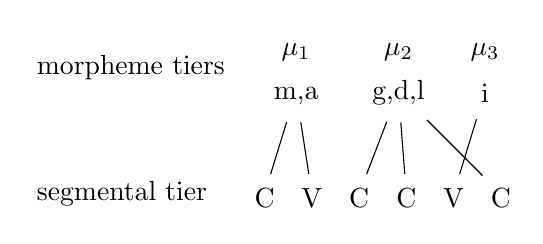
\begin{tikzpicture}[shorten >=2pt,shorten <=3pt, draw=black!100]
	\def \rowthreeht{4.4cm}
	\def \rowtwoht{3.8cm}
	\def \twopointfive{4.1cm}
	%\def \weightstwo{3.75cm}
	\def \rowoneht{2.5cm}
	%\def \weightsone{1.25cm}
	%\def \basement{2cm}
	\tikzstyle{c-node}=[text height=8pt,text centered,inner sep=3pt,minimum size=10pt]
	\tikzstyle{m-node}=[text height=7pt,text centered,inner sep=3pt,minimum size=12pt]
	\tikzstyle{r-node}=[text height=10pt,inner sep=0pt,minimum size=10pt]
	%\tikzstyle{d-node}=[text height=6pt,text centered,inner sep=0pt,minimum size=12pt]
	\tikzstyle{annot}=[text width=25ex,align=left]
	% labels
	\node[annot] (mtierstop) at (0cm,\twopointfive) {morpheme tiers};
	\node[annot] (segtier) at (0cm,\rowoneht) {segmental tier};
	%\node[annot] (mtiersbot) at (0cm,\basement) {};
	
	% surface layer
	\node[r-node] 	(r0)	at (1.0cm,\rowoneht)		{C};
	\node[r-node] 	(r1)	at (1.6cm,\rowoneht)		{V};
	\node[r-node] 	(r2)	at (2.2cm,\rowoneht)		{C};
	\node[r-node] 	(r3)	at (2.8cm,\rowoneht)	 	{C};
	\node[r-node] 	(r4)	at (3.4cm,\rowoneht)	 	{V};
	\node[r-node] 	(r5)	at (4.0cm,\rowoneht)	 	{C};
	
	% hidden-layer elements
	\node[r-node] 	(m0)	at (1.4cm,\rowthreeht)		{$\mu_{1}$};
	\node[r-node] 	(m1)	at (2.7cm,\rowthreeht)		{$\mu_{2}$};
	\node[r-node] 	(m2)	at (3.8cm,\rowthreeht)		{$\mu_{3}$};

	% hidden layer
	\node[c-node] 	(m3)	at (1.4cm,\rowtwoht)		{\/m,a\/};
	\node[c-node] 	(m4)	at (2.7cm,\rowtwoht)		{\/g,d,l\/};
	\node[c-node] 	(m5)	at (3.8cm,\rowtwoht)		{\/i\/};
		
	\path
		(m3)	edge	node	{}	(r0)
		(m3)	edge	node	{}	(r1)
		%
		(m4)	edge	node	{}	(r2)
		(m4)	edge	node	{}	(r3)
		(m4)	edge	node	{}	(r5)
		%
		(m5)	edge	node	{}	(r4);
		
	\end{tikzpicture}
	\label{subfig:nonlinear}
	}

	\subfigure[Linear approach]{
	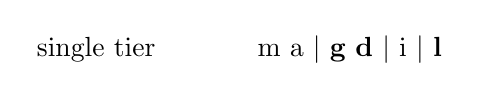
\begin{tikzpicture}[shorten >=1pt,draw=black!100]
	\vspace{50pt}
	\def \floor{0cm}
	\tikzstyle{f-node}=[text centered,inner sep=0pt] %text centered]
	\tikzstyle{annot}=[text width=34ex,align=left]
	% labels
	\node[annot] (floorlabel) at (0cm,\floor) {single tier};
	
	% surface layer
	\node[f-node] 	(f0)	at (1.4cm,\floor)			{m\,\,a\,\,$|$\,\,\textbf{g}\,\,\textbf{d}\,\,$|$\,\,i\,\,$|$\,\,\textbf{l}};
	\end{tikzpicture}
\label{subfig:linear}
}
\caption{Multiple tiers vs. a single tier}
\label{fig:linear}
%\vspace{-20pt}
%\vspace{1pt}
\end{figure}

Notice that $\mu_2$, the consonantal root, is discontinuous; it is
interrupted by $\mu_3$. If a model should have only one tier, as in
fig.~\ref{subfig:linear}, there would be no way of representing the
unity of $\mu_2$, i.e., the fact that \textit{g}, \textit{d}, and \textit{l}
all belong to the same morphological unit. Multiple tiers are thus crucial. With this multi-tier aspect of
autosegmental morphology in mind, we can state two fundamental criteria for any
model of non-concatenative morphology:

\begin{exe}  \ex \label{ex:properties}\begin{xlist}
	\ex {\textsc{Nonlinearity}}: Morphemes are represented as being separate from the segmental tier.
	\ex {\textsc{Nonsequentiality}}: Each morpheme tier (or node) is orthogonal to---i.e., independent of---all other morpheme tiers.
	\end{xlist}
\end{exe}
% \ex this is one 
%\marginpar{or multilinear}
These criteria, or essential properties,
%\textsc{nonlinear} and \textsc{nonsequential} 
are basically binary variables; each \emph{must} be either True or False, and each can \emph{only} be True or False.  Each variable thus has two possible values,
giving us $2^2 = 4$ possible combinations of (non)linearity and (non)sequentiality: 
\textbf{nonlinear nonsequential} (NLNS), \textbf{linear nonsequential} (LNS), 
\textbf{nonlinear sequential} (NLS), and \textbf{linear sequential} (LS).

%[We should note that autosegmental morphology has other properties to
%constrain morphological structure, e.g., the well-formedness
%principle; at present, we are not concerned with capturing all aspects
%of autosegmental morphology, but instead in building a generic system
%to which one can later add linguistically motivated constraints.]

\section{Research objectives}
%State primary research objective: 
\subsection{Primary research objective}
My primary objective is to demonstrate that the multilinear architecture of autosegmental theory can be implemented for the purpose of ULM. That is, my goal is 
to devise \emph{at least one} way of doing this and 
to demonstrate that it works. In particular, I intend to show 
%that the crucial components of autosegmental theory, i.e., 
%those components that allow it to handle non-concatenative morphology, 
that the properties of nonlinearity and nonsequentiality
can be implemented in the form of 
a Multiple Cause Mixture Model (MCMM), 
%which is 
%a general unsupervised learning framework developed by \cite{saund:94}. 
a general unsupervised learning framework developed by \cite{saund:94}. 
I shall thus develop a machine-learning system that is driven by an MCMM.
Its input data will consist of Modern Hebrew words represented as feature vectors. 
I am focusing on Modern Hebrew because 
it exhibits both concatenative and non-concatenative morphological processes 
and thus provides a good test of the method's generality.

\subsection{Secondary research objectives}
\label{sec:secondary-objectives}
My secondary research objectives are outlined below. They are largely concerned with matters of implementation. 
	 \paragraph{Features.} There is a great deal of information tacitly present in a string of alphabetic symbols.
	 This is true regardless of whether the string is written, in which case the symbols are graphemes, or spoken,
	 in which case they are phonemes. In either case, the symbols are each drawn from an alphabet of size $N$ and arranged along a single axis (say, the $x$ axis).
Consider the string of graphemes printed below.
\begin{figure}[h]
	\centering
	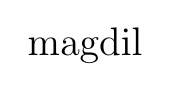
\begin{tikzpicture}[shorten >=2pt,shorten <=3pt, draw=black!100]
	\Large
	\def \rowoneht{0cm}
	\def \rowtwoht{-0.8cm}
	\tikzstyle{r-node}=[text height=10pt,inner sep=0pt,minimum size=10pt]
	%\node[r-node] 	(r0)	at (0cm,\rowoneht)		{\textipa{magdil}};
	\node[r-node] 	(r0)	at (0cm,\rowoneht)		{magdil};
	%\node[r-node] 	(r0)	at (0cm,\rowoneht)		{s t o p};
	%\node[r-node] 	(r0)	at (0cm,\rowtwoht)		{p o t s};
	\end{tikzpicture}
\end{figure}

This row of six graphemes contains a vast amount of tacit information. For instance, suppose we had to represent the string \textit{magdil} not as sequence of alphabetic symbols, but as a series of simple declarative statements. We might come up with statements like the following: 
%These statements might say that a certain character is present in the string, that one character precedes another character, that a particular character occurs at a particular position in the string, and so on, as in the following examples.
\begin{itemize}
  \item \textit{a} immediately follows \textit{m}, \textit{g} immediately follows \textit{a}, \textit{d} immediately follows \textit{g}, and so on. 
  \item \textit{i} immediately precedes \textit{l}, \textit{d} immediately precedes \textit{i}, and so on. %What's more, we know that
   \item \textit{g} follows both \textit{m} and \textit{a}, \textit{d} follows \textit{m}, \textit{a}, and \textit{g}; \textit{d} precedes both \textit{i} and \textit{l}, \textit{g} precedes \textit{d}, \textit{i}, and \textit{l}, and so on.
   \item \textit{m} is the first character, \textit{a} is the second, \dots \textit{i} is the second-to-last character, and \textit{l} is the last character, and so on.
   %\item \textit{l} is the sixth character, \textit{i} is the fifth, \textit{d} is the fourth, and so on.
   \item \textit{m} precedes \textit{a}, \textit{m} precedes \textit{g}, \textit{m} precedes \textit{d}, \dots, \textit{m} precedes \textit{l}; \textit{a} precedes \textit{g}, \dots , \textit{a} precedes \textit{l}; and so on.
   \item \textit{m} is present, \textit{a} is present, \textit{g} is present, and so on.
   \item \emph{ad infinitum}
\end{itemize}
A string of alphabetic symbols tacitly conveys all of these facts and many more---perhaps infinitely more.
Statements like these are essentially what we call \emph{features}.
Each statement can be either true or false, which is to say that each feature is \emph{binary}, drawn from an alphabet of size $N = 2$.  
Many machine learning models require that each input object or \emph{learning instance} (in our case, each \emph{word}) be represented as a vector of binary features, not alphabetic features. Moreover, all input objects (learning instances) must be described by the same feature set, and all feature vectors must be of the same length.

One cannot, of course, have an infinite number of features, as feature vectors must be finite in length.
Now, let $F$ be the infinite set of all possible features. In keeping with the spirit of my primary research objective, we shall assume that there exists at least one $\phi$ such that that $\phi \subset F$, $\phi$ is finite, and $\phi$ allows an ULM system to learn a multilinear model of morphology. The objective here is to confirm this assumption, i.e., to find such a subset.

\paragraph{Data Representation.} The features are extracted from raw-text data, wherein Hebrew words are represented as strings of alphabetic symbols, and the symbols are drawn from a particular alphabet. Now, it so happens that we have more than one alphabet at our disposal, and thus more than one way to represent the input data. These alphabets are the following:
	\begin{enumerate}
		\item \textbf{Modern Hebrew standard orthography}, as transliterated to ASCII characters in the Hebrew Treebank \citep{simaan-et-al:2001}. In the orthography of Modern Hebrew, certain consonants are regularly appropriated to represent vowels. For example, the Hebrew letter
		\textcjheb{w}, transliterated as \textit{w} in the Hebrew Treebank, is by default the consonant /v/, but it is also used to represent the vowels /o/ and /u/. In most syllables, however, the vowel is not represented at all. 
		\item \textbf{Phonemic transcriptions}, i.e., phonemically transcribed words. I have extracted two lists of phonemically transcribed words from the Hebrew portion of the CHILDES database \citep{macwhinney:2000a}. 
		 These lists are the same except that stress is marked in one, but not in the other.
	\end{enumerate}
	%The phonemic transcriptions amount to 12,494 words.
	The question is which mode of representation yields better feature vectors. This is equivalent to asking which mode delivers the largest quantity of useful information and/or the smallest quantity of irrelevant information.
	\paragraph{Mixing and Objective Functions.} The \textbf{mixing function} 
is essentially a voting rule \citep{saund:94}. It prescribes the method whereby the 
``votes" of  hidden units are combined to turn a particular feature (i.e., surface unit) \textsc{on} or \textsc{off} (see section~\ref{sec:mixing-function}. The \textbf{objective function} measures the discrepancy---or, alternatively, similarity---between the surface units' activities and their target activities. 
It thus drives the model's learning by way of trial and error. Objective functions can 
be either positive or negative. Positive objective functions measure similarity and thus 
need to be maximized. Negative objective functions measure error and thus need to be minimized (see section~\ref{sec:mcmm-learning}).

I intend to experiment with two radically different mixing functions, 
viz. one that combines hidden-unit activities linearly and one that combines them nonlinearly.
%(see section~\ref{sec:mixing-function}). 
Similarly, I intend to try out 
%two radically different objective functions, namely 
both a negative and a positive % one (see section~\ref{sec:mcmm-learning}).
objective function. %(see section~\ref{sec:mcmm-learning}).
%Why: What does the mixing function do? What would happen if there were no mixing function? The mixing function maps the hidden-unit activities
%What does the objective function do? What would happen if there were no objective function? 
%If there were no objective function, there could be no learning. Learning proceeds by trial and error. 
%The objective function supplies the error.

\paragraph{Evaluation.} The system described in this proposal is an unsupervised learning system and is thus inherently difficult to evaluate, as one goal of unsupervised learning is to discover previously unknown categories \citep{parsons:2004}.
The previously unknown categories in this case are going to be morphological units of some kind.
However, these units will not be conventional morphemes or morphosyntactic categories. 

Instead, MCMM-generated clusters will correspond roughly to Aronoff's 
\emph{morphomes} \citep{aronoff:1994}, which can be described as \emph{pre-morphosyntactic} units, i.e.,
units that have been assembled from phonemes, but have not yet been assigned 
a syntactic or semantic meaning. I shall use the term \emph{morph} instead of 
\emph{morphome}, however, since MCMM-generated clusters may not correspond 
precisely to morphomes in every case (see section~\ref{sec:targets}).

Thus, the evaluation itself presents an important research question, namely the question of how to evaluate the output of an unsupervised morphological clustering algorithm, particularly one that considers only features of \emph{word-internal form}, having no access to word-external morphosyntactic features, e.g., the person, number, and gender of  surrounding words.

%Thus, my system will not require morphological building blocks to have particular
%meanings. Instead, it 
%My system will thus look for \emph{pre-morphosyntactic} 
%units, i.e., ones assembled from phonemes, but not yet assigned 
%a syntactic or semantic meaning. In a larger pipeline, such 
%building blocks could serve as an interface between morphosyntax 
%and phonology. For instance, while an MCMM can find Hebrew's default 
%masculine suffix \textit{-im}, it cannot say whether it is
%masculine or feminine in a given word, as this suffix
%also occurs in idiosyncratic feminine plurals. The extrinsic part of the evaluation will examine my system's utility as a component within such a pipeline
%(see section~\ref{sec:paradigms}).
%\emph{morphs}. \marginpar{I have yet to introduce morphs, tho} We do not know 
%beforehand \emph{exactly} what these morphs ought to look like. Since we cannot know 
%the ``right answers" before the experiments are run, there can be no clear gold 
%standard against which to evaluate the MCMM's output. 
%
%Thus, the evaluation itself presents an important research question, namely the question of how to evaluate the output of an unsupervised morphological clustering algorithm, particularly one that considers only features of \emph{word-internal form}, having no access to word-external morphosyntactic features, e.g., the person, number, and gender of  surrounding words. Such an algorithm will inevitably produce clusters that do not correspond to abstract morphosyntactic categories or conventional morphemes.
%which are fundamentally morphosyntactic in nature even though the correspondence between morphemes and abstract, or ``atomic," morphosyntactic categories is not always one-to-one.

\chapter{LITERATURE REVIEW}

%\begin{figure}[htb]
%  \centering
%  \begin{tikzpicture}[->,>=stealth',shorten >=1pt,auto,node distance=2.75cm,
%        thick,main node/.style={rectangle,draw,minimum size=1cm,inner sep=0pt]}]
%% \begin{tikzpicture}[
%%            >= stealth, % arrow head style
%%            shorten > = 1pt, % don't touch arrow head to node
%%            auto,
%%            node distance=2.5cm, % distance between nodes
%%            semithick % line style
%%        ]
%%    \node[shape=rectangle,draw=black] (A) at (0,0) {};
%%    \node[shape=rectangle,draw=black] (B) at (2,0) {};
%%    \node[shape=rectangle,draw=black] (C) at (4,0) {};
%%    \node[shape=rectangle,draw=black] (D) at (6,0) {};
%      \node[main node] (1) {};
%    \node[main node] (2) [right of=1]  {};
%    \node[main node] (3) [right of=2] {};
%    \node[main node] (4) [right of=3] {};
%%    \path [->] (A) edge node[right] {} (B);
%%    \path [->] (B) edge node[right] {} (C);
%%    \path [->] (C) edge node[right] {} (D);
%    \path[->]
%    (1) edge node {} (2)
%        %edge node {} (3)
%    (2) edge node {} (3)
%        %edge node {} (3)
%    (3) edge node {} (4);
%        %edge node {} (2);
%  \end{tikzpicture}
%  \caption{A picture of the same gull
%           looking the other way!}
%\end{figure}


\label{sec:rel-work}
\cite{mccarthy:1981} notes a fundamental flaw in linear, strictly concatenative approaches to morphological analysis: 
Because such approaches acknowledge only a single level of representation, the segmental string, they are forced to represent within the same string both the linear order of phonemes and their grouping into morphemes. This effectively binds morphological grouping to the linear order of phonemes, leaving a linear analysis 
%A linear analysis 
with no straightforward means of identifying a discontiguous phoneme sequence as a unified morpheme.
%---i.e., as a single unit with a single, unified set of properties.

%they  However, as we saw in the case of Hebrew, morphemes are not always contiguous.
%As noted by \cite{mccarthy:1981}, strictly concatenative approaches to
%morphology acknowledge only a single level of representation, the
%segmental string.
% (roughly, the string of phonemes). 
%Consequently, they must represent both the %linear 
%order of characters
%(or phonemes) and their morphological grouping within the same linear
%string.
% The problem is that morphemes are not always contiguous, and
% %as we saw above in the case of Hebrew, and 
% %Many languages exhibit non-concatenative processes, and in such cases. 
% a linear analysis has no straightforward means of treating a discontiguous subsequence as a unified morpheme.
%, i.e., as a single unit with a single, unified set of properties.
%, i.e., a truly unified morpheme. 
%McCarthy offers a nonlinear formalism with morphemes represented as
%nodes on autosegmental tiers, allowing

McCarthy thus offers an alternative \emph{nonlinear} formalism in which morphemes are represented as nodes on \emph{autosegmental} tiers, 
i.e., tiers that are separate from the segmental string, allowing
associations between morphemes and phonemes to be independent of phonemes' linear order.
%segments' linear arrangement.
This framework turns out to be highly general, for it uses the same formal machinery to model both 
concatenative and non-concatenative processes; that is, it treats them as essentially the same rather than fundamentally different.

%as fundamentally different; it uses the same formal machinery whether morphemes are contiguous or discontiguous.

% Carry over framework to unsupervised morpheme segmentation?
One can apply McCarthy's ``linear vs. nonlinear" conceptual framework to categorizing existing approaches in ULM.
%Following McCarthy, we 
%distinguish ``linear vs. nonlinear" conceptual framework to categorize existing approaches in ULM.
In the following discussion, we
use the term \textbf{nonlinear} (NL) as a label for algorithms that employ one
or more \textit{hidden layers} to encode the structure of the
\textit{surface layer}.
%, the layer of the graphemes/phonemes.
% Here, \textit{hidden layer} is conceptually related to McCarthy's
% \textit{autosegmental tier}, but the two terms are not necessarily
% equivalent formally.  
We use \textbf{linear} (L) %(cf. ``one-dimensional'') 
to label
algorithms that reference only the surface layer of graphemes in the representation of
morphological structure, e.g., by annotating the
 surface string itself with morpheme boundary symbols. Note that our sense of \textit{linear} is similar to `one dimensional,' which is not necessarily the same as `in/like a (straight) line.'
% This definition is not unlike ``one dimensional," a fairly common
% sense of \textit{linear}.  We do not, however, use \textit{linear} to
% mean ``in/like a straight line."
%but one to be distinguished from ``in/like a straight line." As it is used in this paper, the term \textit{linear} s not related in any direct way to the notions of line and straightness.
%We do not, however, use \textit{linear} to mean ``in a straight line" or even ``like a straight line."
%

We further divide the categories
\textit{linear} and \textit{nonlinear} each into
\textbf{sequential} and \textbf{non-sequential} subcategories:
%, obtaining four categories in all. We describe each below.
An algorithm is sequential (S) if there is a necessary sequence to its morphological classification decisions, i.e., if its decisions are ordered so that for every two decisions, one must precede the other.\footnote{By \textit{morphological 
%if its makes morphological classification decisions depend on preceding or succeeding context, i.e., if there is a necessary sequence to its decisions.
%presentational unit (or feature) depends on the immediately preceding unit(s). %the value of each representational unit is determined independently of all other units
classification decision}, we mean any decision that maps an atomic representational unit (usually a character or a feature) to a morphological category. This definition includes simple ``split" decisions, where there are only two possible categories: ``part of the current morpheme" and ``part of the next morpheme."}
On the other hand, in a non-sequential (NS) algorithm, all morphological classification decisions are made in parallel; i.e., the decisions are unordered.

%is made images these mapping decisions in parallel. That is,  morphemes  in decisions in parallel, the value each representational unit is computed independently of all other units,
%, and thus the immediate context of a given unit is not the predominant factor that determines its value. 
%i.e., if the values of all units are determined in parallel rather than in sequence.
%with each prediction depending on the prediction(s) for the preceding unit(s).
%\begin{itemize}
%\item Given a sequence of morpheme classification decisions, each decision depends on the preceding chain of decisions.
%\item Given a sequence of candidate morpheme split points, each split decision depends on the preceding chain of split decisions. either the preceding representational units or succeither immediately left or immediately right), where \textit{representational unit} is a grapheme if the algorithm is linear and a hidden variable if the algorithm is nonlinear. 
% A \textit{morpheme segmentation decision} is, broadly speaking, an answer to the question, ``What is the morphological category/status of the current representational unit? (e.g., Does the current unit begin a new segment?)"
%\item The dependencies in the sequence all go in the same direction.
%\end{itemize}
 We thus have a total of four categories: linear sequential (LS),
 linear non-sequential  (LNS), non-linear sequential  (NLS), and finally
 non-sequential nonlinear (NLNS). In what follows, we describe each of these in turn.

%We will now discuss and exemplify each of these categories in turn.

\section{linear sequential algorithms}
\label{subsec:seq-lin}

The linear sequential (LS) type of algorithm is depicted in figure~\ref{fig:seq-lin}. 
LS algorithms consider only one layer of representation, namely the surface layer. They use no hidden layers, hence their linearity. The surface layer is made up of surface units, depicted as squares in figure~\ref{fig:seq-lin}.
In LS algorithms, these squares are usually the characters themselves. 
The task is to assign each character to a morphological class. Thus, in effect, 
each square represents a morphological classification decision.
The arrows indicate the sequential order of the algorithm's decisions. 
The fact that there is such an order is the reason this type of algorithm is sequential.
%It is linear because it uses no hidden layer, acknowledging only the surface layer of characters. 
%nthe order in which the algorithm processes the characters. Since the task is to assign each character to a morphological class, each square in effect represents a kind of morphological classification decision. Importantly, there is only one layer of representation, namely the surface layer of characters, hence the linearity of this type of algorithm. Its sequentiality 
%representend in figure~\ref{fig:seq-lin},
%forms morphological hypotheses on the basis of sequential evidence; each prediction depends on immediately preceding
% The circles are positions or character positions (or characters). What do the arrows represent? dependencies. But what depends on what? Maybe the circles are classification decisions, i.e., is character x part of morpheme y? What is it that LS algorithms are typically trying to do? Morpheme-boundary detection/segmentation.
%decisions. Furthermore, LS algorithms acknowledge only the surface layer.
%as well as the evidence informing these decisions, are restricted to the surf
%there is no hidden layer.
% The first unsupervised morpheme segmentation algorithms were linear sequential algorithms.
%The earliest example is the Letter Successor Variety (LSV) method
%\citep{harris:1955, harris:1967}.

The first unsupervised morphological learners were LS algorithms. The earliest examples employed the Letter Successor/Precessor Variety (LSV/LPV) measures \citep{harris:1955, harris:1967}. 
Both measures are intended to indicate likely affixes.
$\text{LSV}(x)$ is intended to find prefixes; given a string $x$ and corpus $W$, $\text{LSV}(x)$ returns the number of letter types that immediately follow $x$ whenever $x$ is word-initial in $W$.
%Both iterate over a corpus $W$.
%$\text{LSV}(x)$ is used to measure the likelihood that the string $x$ is a prefix. and is computed as follows: Given a string $x$ and corpus $W$, $\text{LSV}(x,W)$ iterates over the words $w \in W$, tallying up the letter \emph{types} that occur in the position immediately following $x$ whenever $x$ is word-initial.
%Given a corpus of words $W$ and a string $x$, $\text{LSV}(x,W)$ is the number of letter \textit{types} 
%(as opposed to \textit{tokens}) 
%that found in the position immediately following $x$ whenever $x$ begins a word in $W$.
%the immediately follow $x$ whenever $x$ is word-initial in $W$. 
Letter Predecessor Variety (LPV) is essentially the same measure, except that its function is to find suffixes:
%That is, LPV is simply LSV from the opposite direction: 
it counts the grapheme types that immediately \emph{precede} $x$ whenever $x$ is \emph{word-final}.
%$\text{LSV}(x,W)$ is used to find prefix-stem boundaries, and $\text{LPV}(x)$ to find stem-suffix boundaries. 


% Given a corpus
% %  $W$
% and a string $x$, $\text{LSV}(x)$ is the number of letter
% \textit{types}
% %(as opposed to \textit{tokens}) 
% that occur in the next position following $x$ whenever $x$ is an
% initial substring of a word.
% $w$ in $W$.
% Letter Predecessor Variety (LPV) is the same measure, except the substring $x$ is word-final rather than word-initial, and the direction of the algorithm is reversed. 
% $\text{LSV}(x)$ is used to find prefix-stem boundaries, while $\text{LPV}(x)$ is used to find stem-suffix boundaries.
%
% Stress sequential nature of algorithm
%The different techniques for using LSV to discover morpheme boundaries
%%, such as the ``peak and plateau'' technique
%\citep[see][]{hammarstrom:2011} rely on the intuition that at any
%given point within a morpheme, the next letter is fairly predictable,
%i.e., has a smaller number of succeeding letter types.
%% But at the border between two morphemes, the
%% next letter is much less predictable.
%More recent linear sequential methods
%%have thus abandoned LSV/LPV, often in favor of
%use frequency-based heuristics, such as pointwise mutual information

% Stress sequential nature of algorithm
By themselves, of course, LSV and LSP are merely counts; they must be ``unpacked" if they are to be used to discover legitimate morpheme boundaries.
There are a few different techniques for doing this
%using LSV/LSP to discover morpheme boundaries 
\citep[see][]{hammarstrom:2011}; one is the ``peak and plateau" technique. The following describes the use of peak and plateau with LSV: 
%The following is the peak-and-plateau procedure for finding morpheme boundaries in a word $w$ of the corpus $W$. Suppose the graphemes of $w$ are indexed from 0 to $n$, so that $w[0:2]$, for example, represents the 3-letter string spanning indices 0 to 2. 
%\begin{itemize}
%\item Compute $\text{LSV}(w[0:i], W)$ for each $i$ in the range $[0, n)$.
% \item Insert a morpheme boundary after the substring $w[0:i]$ if and only if $\text{LSV}(w[0:i-1]) \le \text{LSV}(w[0:i]) \ge \text{LSV}(w[0:i+1])$, i.e., there is a local peak in the LSV sequence at index $i$.
%\end{itemize}
\begin{itemize}
\item Given an $n$-length word $w$ whose graphemes are indexed from 0 to $n$, compute $\text{LSV}(w[0:i])$ for each $i$ in the range $[0, n)$.
%in the range $[0, n)$. 
\item Then, for each $i$ in $[0, n)$, insert a morpheme boundary after the substring $w[0:i]$ if and only if 
\begin{equation*}
\text{LSV}(w[0:i-1]) \le \text{LSV}(w[0:i]) \ge \text{LSV}(w[0:i+1]),
\end{equation*}
i.e., there is a local peak in the LSV sequence at index $i$.
\end{itemize}

It is not difficult to see the sequentiality and linearity of an LSV/LPV technique like peak and plateau.
% are not difficult to see.
Such a technique is sequential because its decision making process is shaped by the sequential order of graphemes.
%its decision-making process is to a large extent informed by sequential r graphemes is central to its decision-making process.
%process words as ordered sequences of symbols. bound to make their segmentation decisions in a certain order. This order is imposed by the definition of either LSV or LPV. 
An LSV technique, for example, must proceed left to right, one index at a time, because the LSV calculation at index $i$ depends on the preceding $i-1$ graphemes. Moreover, in peak and plateau, the question of whether or not to draw a morpheme boundary at index $i$ depends not only on the LSV at $i$, but also on the preceding and succeeding LSVs. LSV/LPV techniques are linear because they incorporate no hidden nodes and thus have no means of mediating associations between nonadjacent characters.
% process a string sequence of segmentation decisions proceeding either left to right or right to left, advancing one index at a time that is, at each $i$, the LSV count depends on the preceding $i-1$ graphemes. Notice also the technique's linearity:
%
%Notice the sequential nature of this technique: The algorithm makes a sequence of segmentation decisions proceeding left to right, advancing one index at a time. This left-to-right order is imposed by the definition of LSV; that is, at each $i$, the LSV count depends on the preceding $i-1$ graphemes. Notice also the technique's linearity:
%It has no hidden nodes and thus has no means of mediating associations between discontiguous substrings.
%; at each $i$, for instance, the algorithm can only ``see" the LSVs at $i-1$ and $i+1$
%starting at index 0. The definition of LSV makes  index $0$ to the final index$i$.
%A morphological classification decision is made at each index $i$ starting at the first index of the word in question and ending at the final index. 
%There is a necessary order to this chain of decisions because each decision must consider not only the LSV at $i$, but also the immediately preceding and succeeding LSVs
%First, the LSV count at each $i$ depends on the preceding $i-1$ graphemes. Then, a segmentation decision is made at each $i$
%each LSV calculation is determined solely by the immediately preceding string of graphemes. Note also its linearity: there is only a single layer of representation for both the grapheme sequence and the morphological analysis.

%The intuition behind the LSV/LPV method is essentially the same as that behind the entropy-based methods:
%in natural language processing:
%In fact, LSV generally increases/decreases as entropy increases/deceases:
The intuition behind the LSV/LPV method is that \emph{within} a morpheme, the identity of each letter depends on the letters that immediately precede or succeed it. But this is not the case \emph{between} morphemes. That is, the first letter of a morpheme is largely unpredictable given its preceding letters. Likewise, a morpheme's final letter is largely unpredictable given its succeeding letters. Thus, the number
 of possible letter types tends to increase sharply at the boundary between two morphemes.
%---and hence a larger LVP/LSV---at the boundary between two morphemes. 
%At any given point \emph{within} a morpheme, the next letter is fairly predictable, which generally coincides with a smaller number of succeeding letter types. But at the border between two morphemes, the next letter is much less predictable. This low predictability generally translates to a much larger set of options for the succeeding letter (i.e., a higher LSV). 
However, while morpheme boundaries generally coincide with high LVP/LSV counts, it is not necessarily true that a high LVP/LSV indicates a morpheme boundary.
%LSV is not always a reliable indicator of morpheme boundaries. 
\cite{hammarstrom:2011}, for example, provide LPV counts for the word \textit{disturbance}. 
The highest LPV count of 25 
%(i.e., 25 of the 26 possible letters in the English alphabet) 
occurs between \textit{disturbanc} and \textit{e}.
An LPV-based analysis would thus incorrectly identify \textit{e} as a suffix, a consequence of the ubiquity of \textit{e} as a stem-final letter in English spelling. 

%Goldsmith
Because of such problems, most linear sequential methods today have abandoned LSV/LPV, often in favor of frequency-based heuristics.
\cite{goldsmith:2001}, for example, uses a score based on pointwise mutual information (PMI) to approximate the likelihood that a given character $n$-gram $c_{1}c_{2}...c_{n}$ is a morpheme. 
%In particular, the PMI of the characters $c_{1}, c_{2}, ..., c_{n}$ is multiplied by the relative frequency of the $n$-gram $c_{1}c_{2}...c_{n}$. 
\cite{goldsmith:2001} obtains candidate suffixes (intended for further processing) by taking the $n$-grams that are ranked highest according to this score.  
%(i.e., the count of $c_{1}c_{2}...c_{n}$ divided by the total count of all $n$-grams). 

%Moon
\cite{moon-et-al:2009} apply tree data structures known as \textit{tries} to the task of finding stems and affixes, as have a number of other researchers \citep[e.g.,][]{schone-and-jurafsky:2000, monson:2004, argamon:2004}.
Tries are useful for learning concatenative morphology because they compactly store recurring character sequences.
%that are repeated a group of words. by sets of words beginning with the same character. 
Each node in a trie represents a certain prefix string (with the root node representing the empty string), 
and every path proceeding out from a node represents a possible succeeding character. 
Thus, even though tries are tree data structures, they process data in a sequential manner. 
They 
%also represent morphological relationships linearly 
are linear
because they lack hidden nodes, and every path through a trie is deterministic. 
 \cite{moon-et-al:2009} depart from other trie-based methods in using document 
 boundaries to approximate semantic context. 
 This helps them weed out spurious analyses like the \textit{disturbanc}+\textit{e} 
 example above, but it does not change the fundamentally sequential and linear nature of their approach.
%\citep{goldsmith:2001} or trie-based affix-finding
%\citep{moon-et-al:2009}.
% , for example, uses a score based on pointwise mutual information
% (PMI) to approximate the likelihood that a given character $n$-gram
% %$c_{1}c_{2}...c_{n}$ 
% is a morphemic unit.
% In particular, the PMI of the characters $c_{1},
% c_{2}, ..., c_{n}$ is multiplied by the relative frequency of the
% $n$-gram $c_{1}c_{2}...c_{n}$. \cite{goldsmith:2001} obtains candidate
% suffixes by taking the $n$-grams that are ranked highest according to
% this score.
%(i.e., the count of $c_{1}c_{2}...c_{n}$ divided by the total count of all $n$-grams).  
%
%Moon
% \cite{moon-et-al:2009} apply tries to the task of finding stems and
% affixes, to store recurring character sequences.
%, as have a number of other researchers. 
% Tries are useful for learning concatenative morphology because they
% compactly store recurring character sequences.
%that are repeated a group of words. by sets of words beginning with the same character. 
% Each node in a trie represents a certain prefix string (with the root node representing the empty string), 
% and every path proceeding out from a node represents a possible succeeding character. 
% Thus, even though tries are tree data structures, 
%In all cases, the methods process data in a sequential manner and
%lack hidden nodes for representing morphological relationships.
% linearly, lacking hidden nodes.

% ; one of them is the ``peak and plateau" technique, which works as follows:
% \begin{itemize}
% \item Given an $n$-length word $w$ whose graphemes are indexed from 0 to $n$, compute $\text{LSV}(w[0:i])$ for each $i$ in the range $[0, n)$. \item Insert a morpheme boundary after the substring $w[0:i]$ if and only if $\text{LSV}(w[0:i-1]) \le \text{LSV}(w[0:i]) \ge \text{LSV}(w[0:i+1])$, i.e., there is a local peak in the LSV sequence at index $i$.
% \end{itemize}
% Notice the sequential nature of this technique: each LSV calculation is determined solely by the immediately preceding string of graphemes. Note also its linearity: there is only a single layer of representation for both the grapheme sequence and the morphological analysis.

 \begin{figure}[tb]
 %\begin{minipage}{.3\textwidth}
 \begin{center}
 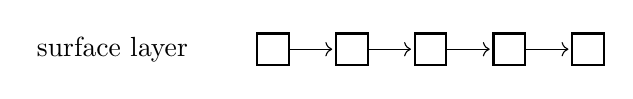
\begin{tikzpicture}[shorten >=1pt,->,draw=black!100,node distance = 1.3cm, auto]]
 	\def \startnode{1.5cm}
 %	\def\secondrow{1.0cm}
 	\tikzstyle{r-node}=[regular polygon sides=4,draw=black!100,thick,inner sep=0pt,minimum size=4mm]
 	\tikzstyle{annot} = [text width=3cm]
 %	\tikzstyle{annot} = [text width=2.0cm, text centered]
 	% labels
 %	\node[annot] (m-label) at (0,\thirdrow) {hidden-unit vector};
 %	\node[annot] (r-label) at (0, \secondrow) {prediction vector};
 %	\node[annot] (d-label) (0, 0) {observed data vector};
 	% hidden layer
 	\node[annot] (surface-label) at (0cm,0cm) {surface layer};
 %	\node[annot] (r-label) at (0, \secondrow) {prediction vector};
 %	\node[annot] (d-label) (0, 0) {observed data vector};
	
 	% surface layer
 	\node[r-node] 	(r0)	at (\startnode,0cm)		{};
 	\node[r-node] 	(r1)	at (2.5cm, 0cm)		{};
 	\node[r-node] 	(r2)	at (3.5cm,0cm)	 	{};
 	\node[r-node] 	(r3)	at (4.5cm,0cm) 		{};
 	\node[r-node] 	(r4) 	at (5.5cm,0cm)   		{};
	
 	\path (r0)	edge	node	{}	(r1)
 		(r1)	edge	node	{}	(r2)
 		(r2)	edge	node	{}	(r3)
 		(r3)	edge	node	{}	(r4);
 \end{tikzpicture}
 \end{center}
 \caption{linear sequential architecture.}
 %. Each representational unit depends on the preceding unit, and no unit exists outside of the surface layer.}
 \label{fig:seq-lin}
 \end{figure}

% The intuition behind the LSV/LPV method is related to that behind the entropy-based methods in natural language processing:
% %In fact, LSV generally increases/decreases as entropy increases/deceases: 
% At any given point \emph{within} a morpheme, the next letter is fairly predictable, which generally coincides with a smaller number of succeeding letter types. But at the border between two morphemes, the next letter is much less predictable. This low predictability generally translates to a much larger set of options for the succeeding letter (i.e., a higher LSV). However, it out that LSV is not always a reliable indicator of morpheme boundaries. \cite{hammarstrom:2011}, for example, provide LPV counts for the word \textit{disturbance}. 
% The highest count (25) 
% %(i.e., 25 of the 26 possible letters in the English alphabet) 
% occurs between \textit{disturbanc} and \textit{e}, An LPV-based analysis would thus yield an incorrect result in this case, a consequence of the fact that \textit{e} is such a ubiquitous word-final letter in English spelling. 

%Goldsmith
% More recent linear sequential methods
% %have thus abandoned LSV/LPV, often in favor of
% use frequency-based heuristics.  \cite{goldsmith:2001}, for example,
% uses a score based on pointwise mutual information (PMI) to
% approximate the likelihood that a given character $n$-gram
% %$c_{1}c_{2}...c_{n}$ 
% is a morphemic unit.
% % In particular, the PMI of the characters $c_{1},
% % c_{2}, ..., c_{n}$ is multiplied by the relative frequency of the
% % $n$-gram $c_{1}c_{2}...c_{n}$. \cite{goldsmith:2001} obtains candidate
% % suffixes by taking the $n$-grams that are ranked highest according to
% % this score.
% %(i.e., the count of $c_{1}c_{2}...c_{n}$ divided by the total count of all $n$-grams).  
% %
% %Moon
% \cite{moon-et-al:2009} applies \textit{tries} to the task of finding stems and
% affixes, to store recurring character sequences in the search for recurring character sequences.
% % A number of other researchers have done the same.
% % Tries are useful for learning concatenative morphology because they
% % compactly store recurring character sequences.
% %that are repeated a group of words. by sets of words beginning with the same character. 
% % Each node in a trie represents a certain prefix string (with the root node representing the empty string), 
% % and every path proceeding out from a node represents a possible succeeding character. 
% % Thus, even though tries are tree data structures, 
% In all cases, the methods process data in a sequential manner and
% represent morphological relationships linearly, lacking hidden nodes.

% , and every path through a trie is deterministic.
% \cite{moon-et-al:2009} depart from other trie-based methods in using
% document boundaries to approximate semantic context.  This helps them
% weed out spurious analyses like the \textit{disturbanc}+\textit{e}
% example above, but it does not change the fundamentally sequential and
% linear nature of their approach.

\section{inear non-sequential algorithms}
\label{subsec:nonseq-lin}
In the linear non-sequential  (LNS) type of algorithm, shown in figure~\ref{fig:nonseq-lin}, the representational units are generally not raw characters, but rather \emph{features}, i.e., binary variables representing the presence or absence of particular properties.
%specifying whether or not a word has a certain property. 
Features in non-sequential algorithms need not correspond to contiguous chunks of the original string; for example, features like the following are perfectly valid: ``\textit{t} precedes \textit{i} within $\delta$ characters" and ``\textit{t} precedes \textit{b} within $\delta$ characters," where the character pairs \emph{t..i} and \emph{t..b} are discontiguous as long as $\delta \ne 0$. Notice that such features cannot really be ordered; each is either \textsc{true} or \textsc{false} irrespective of order.
All non-sequential algorithms---of which LNS algorithms are a subcategory---view a given word's features as being unordered, i.e., as being sequentially unrelated to each other. 
But while LNS algorithms are non-sequential, they are linear because they incorporate no hidden units. Thus, even though an LNS algorithm's features may refer to discontiguous subsequences of characters, they are nonetheless restricted to representing only properties that are overtly present in the surface layer of characters. 

One LNS example is the algorithm of \cite{poon-et-al:2009}, which uses log-linear models to induce morphological segmentations for Arabic and Hebrew. 
Log-linear models are inherently non-sequential because they treat all features as independent, estimating a global joint probability for the entire bag of features. 
%Sequential models, in contrast, estimate conditional probabilities based on sequential dependencies between features
The algorithm of \cite{poon-et-al:2009} in particular searches for the set of parameters $\theta$ that maximizes the joint probability of a corpus $W$ and a morphological segmentation $S$, i.e., $P(W,S| \theta) = P(W|S; \theta) \cdot P(S| \theta)$. The segmentation $S$ is encoded by a set of features.
%They generate candidate segmentations via Gibbs sampling. For each candidate, they extract a feature set

%Log-linear models are well-suited for large numbers of arbitrarily defined features. 
\cite{poon-et-al:2009} use two categories of features to encode a morphological segmentation: \textit{morpheme features} and \textit{morpheme context} features.
The former encode (potential) morpheme types and their frequencies, e.g., \texttt{vlAv:5} and \texttt{w:31}. The 
latter encode context types and their frequencies, where a \emph{context} consists of the $n$ characters preceding and succeeding a (potential) morpheme;
%the character bigrams to the left and right of a potential morpheme, 
e.g., the feature \texttt{\#w\_wn:12} would represent a context whose left side consists of \textit{w} preceded by the word boundary, whose right side is the bigram \textit{wn}, and whose frequency is 12. Importantly, these context features overlap. That is, in \texttt{\#w\_wn:12}, the \textit{w} and \textit{wn} are themselves morphemes whose contexts must be extracted.
This feature overlap is made possible by the non-sequentiality of log-linear models.
%is on the right, , respectively, and whose frequency of this particular context as 12.
%s that the left context is the character \textit{w} preceded by the word boundary, the right context is the character bigram \textit{wn}, and the frequency of this particular context is 12).
% and \textand the characters \textit{w} and \textit{n} are on the right potential morpheme\textit{w} on the left 
%and the characters \textit{w} and \textit{n} on the right).
%Note, however, that 

Note, however, that log-linear models can handle much more non-sequentiality than this. Indeed, since a log-linear models is inherently non-sequential, it accommodate any sort of non-sequential feature. 
%one can incorporate into log-linear model.
%feature %or combination of feature types 
%in a log-linear model.  
One could, for example, incorporate
features representing discontiguous bigrams,
as already noted.
 One could also combine contiguous and discontiguous bigram features in the same feature set.
%for example, have features representing both contiguous and discontinous bigrams in the same feature set.
%However, one in principle could use any sort of feature in a log linear model, such as a feature type representing discontiguous bigrams, for example.
%Each feature represents the both corpus and the segmentation jointly, and a fully specified set of features thus represents an entire segmented corpus;
%but there is no limit on the variety or quantity of features one can incorporate into a log-linear model.
% Why is a log linear model non-sequential?
%Log-linear models are inherently non-sequential because they treat all features as independent, estimating a global joint probability for the entire bag of features. Sequential models, in contrast, estimate conditional probabilities based on sequential dependencies between features.
% Why is a log linear model non-sequential?
And yet it is not the nature of the features themselves that makes an algorithm non-sequential, but rather the lack of sequential relationships between features. The algorithm of \cite{poon-et-al:2009} is non-sequential because it does not process features in a particular order.
% Why is Poon et al's algorithm linear?
It is, however, linear because it incorporates no hidden units to mediate associations between features.

%\cite{poon-et-al:2009} incorporate no latent variables, however. 
%Their representation of morphological structure makes reference only to the the surface layer of graphemes. Their morpheme features are limited to  contiguous grapheme sequences, 
%and their morpheme context features encode only extreme left and right contexts, 
%thus assuming no internal boundaries (i.e., no morpheme interruptions).
%%They generate candidate segmentations via Gibbs sampling, but, for an $n$-length word, they consider 
%Because it only acknowledges the surface layer of text, the algorithm of \cite{poon-et-al:2009} can only isolate stems and affixes, not the discontiguous roots and patterns of Arabic and Hebrew.

%\paragraph{inear non-sequential algorithms}
%\label{subsec:nonseq-lin}
%
%Like LS algorithms, \textbf{linear non-sequential } (LNS) algorithms consist only of surface units, having no hidden layer, hence their linearity. LNS algorithms are different in that there are no dependencies between representational units. Each unit is independent of other units, hence their \textit{non-sequential} characterization.
%%They consist only of surface units, hence their linearity. What sets LNS algorithms apart is the lack of dependencies between these units, h
%%illustrated in figure~\ref{fig:nonseq-lin}, 
%%there are no dependencies between representational units, but also no
%%hidden units.
%%; i.e., all representational units reside in the surface layer.  
%As one example, \cite{poon-et-al:2009} use log-linear models to induce
%morphological segmentations for Arabic and Hebrew. 
%% Their algorithm
%% searches for the set of parameters $\theta$ that maximizes the joint
%% probability of a corpus $W$ and a segmentation $S$ (i.e., $P(W,S|
%% \theta)$).
%% = P(W|S; \theta) \cdot P(S| \theta)$.
%%They generate candidate segmentations via Gibbs sampling. For each candidate, they extract a feature set
%% Log-linear models are well-suited for large numbers of arbitrarily
%% defined features.
%% \cite{poon-et-al:2009} use morpheme features and morpheme context
%% features.  The former category specifies a morpheme type and its
%% frequency, e.g., \texttt{vlav:1} and \texttt{w:2}.  The latter
%% category indicates the character bigrams to the left and right of a
%% given morpheme, e.g., \texttt{\#w\_wn:1} (a word boundary followed by
%% the character \textit{w} on the left and the characters \textit{w} and
%% \textit{n} on the right).  Note, however, that one could use any type
%% of feature or combination of feature types with a log-linear
%% model. One could, for example, have features representing both
%% contiguous and discontinues bigrams in the same feature set.
%%
%%However, one in principle could use any sort of feature in a log linear model, such as a feature type representing discontiguous bigrams, for example.
%%Each feature represents the both corpus and the segmentation jointly, and a fully specified set of features thus represents an entire segmented corpus;
%%but there is no limit on the variety or quantity of features one can incorporate into a log-linear model.
%% Why is a log linear model non-sequential?
%Log-linear models are non-sequential because they treat all features
%as independent, estimating a global joint probability.
%%for the entire bag of features.
%% Sequential models, in contrast, estimate conditional probabilities
%% based on sequential dependencies between features.
%% Why is Poon et al's algorithm linear?
%% \cite{poon-et-al:2009} incorporate no latent variables,
%% %, however, 
%% %Their representation of morphological structure makes 
%% referencing only the the surface layer of graphemes.
%% Their morpheme
%% features are limited to contiguous grapheme sequences, and their
%% morpheme context features encode only extreme left and right contexts,
%% thus assuming no internal boundaries (i.e., no morpheme
%% interruptions).  
%Even though such a log-linear model allows for any type of feature,
%including both contiguous and discontiguous $n$-grams,
%%They generate candidate segmentations via Gibbs sampling, but, for an $n$-length word, they consider  
%the algorithm ultimately can only isolate stems and affixes, because
%it only acknowledges the surface layer of text.
%%, and not discontiguous roots and patterns.
%% of Arabic and Hebrew.

 \begin{figure}[tb]
 %\begin{minipage}{.3\textwidth}
 \begin{center}
 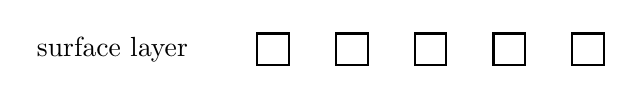
\begin{tikzpicture}[shorten >=1pt,->,draw=black!100]
 	\def \startnode{1.5cm}
 %	\def\secondrow{1.0cm}
 	\tikzstyle{r-node}=[regular polygon sides=4,draw=black!100,thick,inner sep=0pt,minimum size=4mm]
 	\tikzstyle{annot} = [text width=3cm]
 	% labels
 	\node[annot] (surface-label) at (0cm,0cm) {surface layer};
 %	\node[annot] (r-label) at (0, \secondrow) {prediction vector};
 %	\node[annot] (d-label) (0, 0) {observed data vector};
	
 	% surface layer
 	\node[r-node] 	(r0)	at (\startnode,0cm)		{};
 	\node[r-node] 	(r1)	at (2.5cm, 0cm)		{};
 	\node[r-node] 	(r2)	at (3.5cm,0cm)	 	{};
 	\node[r-node] 	(r3)	at (4.5cm,0cm) 		{};
 	\node[r-node] 	(r4) 	at (5.5cm,0cm)   		{};
	
 %	\path (r0)	edge	node	{}	(r1)
 %		(r1)	edge	node	{}	(r2)
 %		(r2)	edge	node	{}	(r3)
 %		(r3)	edge	node	{}	(r4);
 \end{tikzpicture}
 \end{center}
 \caption{inear non-sequential architecture}
 
 %. No dependencies exist between representational units, and no unit exists outside of the surface layer.}
 \label{fig:nonseq-lin}
 \end{figure}

% \cite{poon-et-al:2009} use morpheme features and morpheme context
% features.  The former category specifies a morpheme type and its
% frequency, e.g., \texttt{vlav:1} and \texttt{w:2}.  The latter
% category indicates the character bigrams to the left and right of a
% given morpheme, e.g., \texttt{\#w\_wn:1} (a word boundary followed by
% the character \textit{w} on the left and the characters \textit{w} and
% \textit{n} on the right).  Note, however, that one could use any type
% of feature or combination of feature types with a log-linear
% model. One could, for example, have features representing both
% contiguous and discontinues bigrams in the same feature set.


\section{Sequential nonlinear algorithms}
\label{subsec:seq-nonlin}
% First, what sort of algorithms are sequential nonlinear?
The sequential nonlinear (NLS) type of algorithm is illustrated in figure~\ref{fig:seq-nonlin}. 
Note in particular the addition of a hidden layer, whose units (the circular nodes)
represent the underlying sources of the surface data's implicit structure.
%account for the surface %the surface units and thus take responsibility for the regularities ac
%for 
%algorithms differ from linear sequential ones in that 
%they add a layer of hidden units for 
%encoding 
%take responsibility for generating the structure implicit
%the regularities %, i.e., the implicit structure, 
%in the surface layer and thus the
%data.
%These hidden units can be viewed as causing or generating the surface data.
NLS algorithms are nonlinear because they incorporate a hidden layer.
However, they are sequential because the hidden layer in an NLS algorithm is sequential; i.e., its component hidden units
%hidden units
are sequentially ordered.
Since the surface units depend on the hidden units, the hidden layer imposes its sequential order on the surface layer. 
%they have a certain each hidden unit depends on its predecessor hidden unit(s). 
% I need to say what the nonlinear aspect brings to the table. If being nonlinear is beneficial, sequential nonlinear algorithms should be better than linear sequential ones. So what do sequential nonlinear algorithms have that linear sequential algorithms don't? How does being nonlinear help them?
% First, what sort of algorithms are sequential nonlinear?

%Sequential nonlinear (NLS) algorithms
%%, illustrated in figure~\ref{fig:seq-nonlin}, 
%differ from sequential
%linear ones by adding a layer of hidden units for encoding the
%structure of the surface layer.
%This makes them nonlinear. 
% They are still sequential, however, in that there are sequential
% dependencies within the hidden layer.
%; i.e., each hidden unit depends on its predecessor hidden unit(s).
%The prototypical example of a sequential nonlinear model is the Hidden
%Markov Model (HMM).  \cite{creutz-and-lagus:2005,
%  creutz-and-lagus:2007} employ an HMM to induce a morphological
%lexicon.
The prototypical NLS model is the Hidden Markov Model (HMM). 
\cite{creutz-and-lagus:2005, creutz-and-lagus:2007} employ an HMM to induce a morphological lexicon, i.e., a list of morpheme-like segments they call \textit{morphs}. 
%, i.e., a list of morpheme-like segments.
%that they call \textit{morphs}.
%sorted in order of increasing morph length. 
%They take a maximum a posteriori (MAP) approach.
Their algorithm seeks to find the lexicon such that $P(lexicon|corpus)$ is maximized. Due to Bayes' theorem, this equates to finding the lexicon that maximizes $P(corpus|lexicon) \cdot P(lexicon)$. The probability $P(corpus|lexicon)$ is computed by an HMM. Each unit in this HMM's hidden layer can take on five possible values: \textit{prefix}, \textit{stem}, \textit{suffix}, \textit{word boundary}, and \textit{non-morpheme}. 
Note how the first four relate sequentially to each other: prefixes must precede stems, stems must precede suffixes, and so on.
%The observation sequence is a segmentation hypothesis, i.e., a candidate segmentation of the corpus into morphs. 
%Candidate segmentations are generated independently of the HMM, as are the transition and emission probabilities. 
%The HMM's role to find likely hidden state sequence, which is computed by the Viterbi algorithm, along with the probability $P(corpus|lexicon)$. 
The hidden layer in this case serves to facilitate the search for the optimal lexicon 
(i.e., segmentation) by providing a means of abstracting away from the literal surface characters.

%The HMM's role is to evaluate each candidate morph sequence. 
% took out the "h"
 \begin{figure}[tb]
 %\begin{minipage}{.3\textwidth}
 \begin{center}
 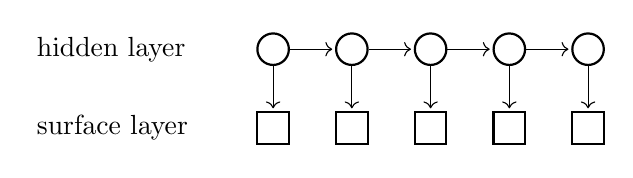
\begin{tikzpicture}[shorten >=1pt,->,draw=black!100]
 	\def \rowtwoht{1.0cm}
 	\def \rowoneht{0.0cm}
 	\tikzstyle{m-node}=[circle,draw=black!100,thick,inner sep=0pt,minimum size=4mm]
 	\tikzstyle{r-node}=[regular polygon sides=4,draw=black!100,thick,inner sep=0pt,minimum size=4mm]
 	\tikzstyle{annot} = [text width=3cm]
 	% labels
 	\node[annot] (hidden-label) at (0cm,\rowtwoht) {hidden layer};
 	\node[annot] (surface-label) at (0cm,\rowoneht) {surface layer};

 %	\node[annot] (d-label) (0, 0) {observed data vector};
	
 	% hidden layer
 	\node[m-node] 	(m0)	at (1.5cm,\rowtwoht)		{};
 	\node[m-node] 	(m1)	at (2.5cm,\rowtwoht)		{};
 	\node[m-node] 	(m2)	at (3.5cm,\rowtwoht)	 	{};
 	\node[m-node] 	(m3)	at (4.5cm,\rowtwoht) 		{};
 	\node[m-node] 	(m4) 	at (5.5cm,\rowtwoht)   		{};
	
 	% surface layer
 	\node[r-node] 	(r0)	at (1.5cm,\rowoneht)		{};
 	\node[r-node] 	(r1)	at (2.5cm,\rowoneht)		{};
 	\node[r-node] 	(r2)	at (3.5cm,\rowoneht)	 	{};
 	\node[r-node] 	(r3)	at (4.5cm,\rowoneht) 		{};
 	\node[r-node] 	(r4) 	at (5.5cm,\rowoneht)   		{};
	
 	\path (m0)	edge	node	{}	(m1)
 		(m1)	edge	node	{}	(m2)
 		(m2)	edge	node	{}	(m3)
 		(m3)	edge	node	{}	(m4);
		
 	\path (m0)	edge	node	{}	(r0)
 		(m1)	edge	node	{}	(r1)
 		(m2)	edge	node	{}	(r2)
 		(m3)	edge	node	{}	(r3)
 		(m4)	edge	node	{}	(r4);
			
 \end{tikzpicture}
 \end{center}
 \caption{Sequential nonlinear architecture}
 % . Sequential dependencies only exist between hidden units, 
 % not between the observed units of the surface layer. The hidden units ``cause" the surface units.}
 \label{fig:seq-nonlin}
 \end{figure}

\section{Non-sequential nonlinear algorithms}
\label{subsec:nonseq-nonlin}
% Intro
 Like sequential nonlinear (NLS) algorithms, \textit{non}-sequential
 nonlinear (NLNS) algorithms incorporate a hidden layer whose units generate the observed
 units of the surface layer.
The difference is that the hidden layer in an NLNS algorithm is \emph{non-sequential}; 
i.e., the algorithm computes the values of all hidden units in parallel rather than in a sequence.
The surface layer in a NLNS algorithm is also non-sequential.
 %dependencies.
 Thus, every unit---whether hidden or surface---is entirely independent
 within its own layer. Figure~\ref{fig:nonseq-nonlin} illustrates the NLNS framework; notice that no two nodes with the same layer are connected by an arc.
This intra-layer independence allows a hidden unit to associate with
any combination of surface units, whether contiguous or discontiguous
%(see Figure \ref{fig:nonseq-nonlin}).

 \begin{figure}[tb]
 %\begin{minipage}{.3\textwidth}
 \begin{center}
 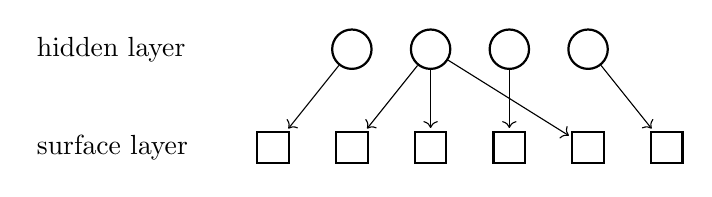
\begin{tikzpicture}[shorten >=1pt,->,draw=black!100] %,scale=.95]
 	\def \rowtwoht{1.25cm}
 	\def \rowoneht{0.0cm}
 	\tikzstyle{m-node}=[circle,draw=black!100,thick,inner sep=0pt,minimum size=5mm]
 	\tikzstyle{r-node}=[regular polygon sides=4,draw=black!100,thick,inner sep=0pt,minimum size=4mm]
 	\tikzstyle{annot} = [text width=3cm]
 	% labels
 	\node[annot] (hidden-label) at (0cm,\rowtwoht) {hidden layer};
 	\node[annot] (surface-label) at (0cm,\rowoneht) {surface layer};

 %	\node[annot] (d-label) (0, 0) {observed data vector};
	
 	% hidden layer
 	\node[m-node] 	(m0)	at (2.5cm,\rowtwoht)		{};
 	\node[m-node] 	(m1)	at (3.5cm,\rowtwoht)		{};
 	\node[m-node] 	(m2)	at (4.5cm,\rowtwoht)	 	{};
 	\node[m-node] 	(m3)	at (5.5cm,\rowtwoht) 		{};
	
 	% surface layer
 	\node[r-node] 	(r0)	at (1.5cm,\rowoneht)		{};
 	\node[r-node] 	(r1)	at (2.5cm,\rowoneht)		{};
 	\node[r-node] 	(r2)	at (3.5cm,\rowoneht)	 	{};
 	\node[r-node] 	(r3)	at (4.5cm,\rowoneht) 		{};
 	\node[r-node] 	(r4) 	at (5.5cm,\rowoneht)   		{};
 	\node[r-node] 	(r5) 	at (6.5cm,\rowoneht)   		{};
	
 	\path (m0)	edge	node	{}	(r0)
 		(m1)	edge	node	{}	(r1)
 		(m2)	edge	node	{}	(r3)
 		(m1)	edge	node	{}	(r2)
 		(m1)	edge	node	{}	(r4)
 		(m3)	edge	node	{}	(r5);
		
 \end{tikzpicture}
 \end{center}
 \caption{Non-sequential nonlinear architecture}
 %. Neither layer contains sequential dependencies; every unit is independent within its own layer. Each hidden unit is thus free to cause any combination of observed units.}
 \label{fig:nonseq-nonlin}
 \end{figure}

%The NLNS type can take many forms.  \cite{baroni-et-al:2002}, for
%example, implicitly detect hidden units by computing edit distance for
%pairs of words.
%% The
%% Levenshtein algorithm finds the minimum number of edit operations
%% (typically allowing substitutions, deletions, and insertions) required
%% to change a \textit{source} word into a \textit{target} word.  In
%% addition to edit distance and edit operations, the algorithm can align
%% the characters of the source with those of the target word.  
%From an alignment, one can extract the two words' (potentially
%discontiguous) common subsequence.  Thus, one may view the alignment
%as showing
%%indicative of
%a single hidden unit behind the surface occurrences of the
%subsequence.  For example, for the Hebrew words \textit{dibr} `he
%spoke' and \textit{mdbr} `he is speaking', the discontiguous root
%\textit{d.b.r} is found.
% Of course, a common subsequence does not necessarily indicate a
% morphological relationship; consider, for instance, the English pair
% To avoid finding spurious relationships
% (cf. \textit{pork}/\textit{park}), \cite{baroni-et-al:2002} compute a
% semantic similarity score, based on mutual information, to combine
% with this orthographic similarity.
% based on minimum edit distance.
%orthographic similarity score.

The NLNS type can take many forms. 
\cite{baroni-et-al:2002}, for example, detect implicit causal units by computing the Levenshtein alignments for pairs of words. 
The Levenshtein algorithm finds the minimum number of edit operations 
(typically allowing substitutions, deletions, and insertions) required to change 
a \textit{source} word into a \textit{target} word.
An alignment of the source and target characters is obtained as a by-product of computing the edit operations. 
%In addition to edit distance and edit operations, the algorithm can align the characters of the source with those of the target word. 
From the alignment, one can extract the (not necessarily contiguous) subsequence held in common by the two words.
%One might view the common subsequence as suggesting a sin
Thus, one may view the alignment as suggesting a single causal unit behind both occurrences of the subsequence, i.e., as a kind of implicit hidden unit, as it were.
For example, the alignment in figure~\ref{fig:lev-align} implies a single cause behind both occurrences of the subsequence \textit{dbr}.
Of course, a common subsequence does not necessarily indicate a morphological relationship; 
consider, for instance, the English pair \textit{pork}/\textit{park}. 
To avoid finding spurious relationships, 
\cite{baroni-et-al:2002} compute a semantic similarity score based on mutual information, 
combining it with an orthographic similarity score based on minimum edit distance.

 \begin{figure}[htb!]
 %\begin{minipage}{.3\textwidth}
 \begin{center}
 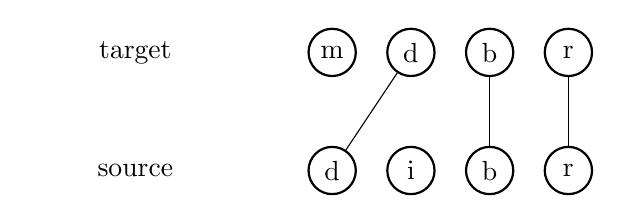
\begin{tikzpicture}[draw=black!100]
 	%[shorten >=1pt,->,draw=black!100]
 	\def \rowtwoht{1.5cm}
 	\def \rowoneht{0.0cm}
 	\tikzstyle{m-node}=[circle,draw=black!100,thick,inner sep=0pt,minimum size=6mm]
 	\tikzstyle{r-node}=[circle,draw=black!100,thick,inner sep=0pt,minimum size=6mm]
 	\tikzstyle{annot} = [text width=2.5cm, text centered]
 	% labels
 	\node[annot] (hidden-label) at (0cm,\rowtwoht) {target};
 	\node[annot] (surface-label) at (0cm,\rowoneht) {source};

 %	\node[annot] (d-label) (0, 0) {observed data vector};
	
 	% hidden layer
 	\node[m-node] 	(m0)	at (2.5cm,\rowtwoht)		{m};
 	\node[m-node] 	(m1)	at (3.5cm,\rowtwoht)		{d};
 	\node[m-node] 	(m2)	at (4.5cm,\rowtwoht)	 	{b};
 	\node[m-node] 	(m3)	at (5.5cm,\rowtwoht) 		{r};
	
 	% surface layer
 	\node[r-node] 	(r0)	at (2.5cm,\rowoneht)		{d};
 	\node[r-node] 	(r1)	at (3.5cm,\rowoneht)		{i};
 	\node[r-node] 	(r2)	at (4.5cm,\rowoneht)	 	{b};
 	\node[r-node] 	(r3)	at (5.5cm,\rowoneht) 		{r};
 	%\node[r-node] 	(r4) 	at (6.5cm,\rowoneht)   		{};
 	%\node[r-node] 	(r5) 	at (7.5cm,\rowoneht)   		{};
	
 	\path (m1)	edge	node	{}	(r0)
 		(m2)	edge	node	{}	(r2)
 		(m3)	edge	node	{}	(r3);
 %		(m3)	edge	node	{}	(r3)
 %		(m1)	edge	node	{}	(r4)
 %		(m3)	edge	node	{}	(r5);
		
 \end{tikzpicture}
 \end{center}
 \caption{The minimum-edit-distance alignment for the Hebrew words \textit{dibr} `he spoke' and \textit{mdbr} `he is speaking'. The discontiguous root \textit{d.b.r } is discovered by aligning \textit{dibr} with \textit{mdbr} and extracting the common subsequence.}
 \label{fig:lev-align}
 \end{figure}


Other authors simulate a nonlinear, multi-tier representation by separating the 
learning process into two or more phases.
The first phase classifies individual literal characters into abstract categories that are then used by a second phase (and perhaps subsequent phases) to perform other aspects of the analysis.
Multiple phases occurring at different times can thus replicate the effects of multiple simultaneous levels of representation.
This is the approach taken by \cite{rodrigues-and-cavar:2005} to induce the non-concatenative morphology of Arabic. 
%Following the statistical constraint-based method of \cite{elghamry:2005}, 
Their first phase identifies root radicals according to the statistical constraint-based method of \cite{elghamry:2005}. 
For each word in their corpus, 
they generate a set of candidate triliteral roots according to 
constraints derived from the tendencies of Arabic roots as observed in corpora. 
In particular, any 3-length subsequence is admitted into the candidate set 
if and only if it satisfies both of the following:
%, which in Arabic comprise both a consonantal root and a vocalic pattern. A string is allowed into a word's candidate stem set if and only if it satisfies the following constraints, which are based on the tendencies of Arabic roots as observed in corpora.
\begin{enumerate} 
\item No two consecutive radicals may be separated by more than two characters.
\item No more than four characters intervene between the first and third radicals.
\end{enumerate}
%\item ``The distance between the first and third radicals cannot be greater than five" \citep[][p. 3]{elghamry:2005}. 
Then, a statistical score is computed for each candidate, and the one with the highest score is selected as the root.
Once the roots---and thus the stems---have been isolated by the first phase, the second phase identifies the concatenative affixes through a separate methodology.

% Goldsmith and Xanthos
An alternative first-phase strategy can be found in \cite{goldsmith-and-xanthos:2009}, 
who present methods for
partitioning a phonemic inventory into a class of consonants and a class of vowels. 
Their paper does not go into automatic morphological analysis, but it is not difficult to see how C and V classes could be useful to a multi-phase morphological analyzer.
The first phase would partition the phonemic inventory and, for each word, label each phoneme/grapheme as either a consonant or vowel, thus creating a sort of CV skeleton similar to the segmental tier of autosegmental phonology.
Subsequent phases would then use these CV skeletons to isolate roots, patterns, and other morphemes.
%The second phase (and perhaps subsequent phases) would then use template to Such a template would be helpful to subsequent phases as they go about isolating the root, pattern, and other morphemes. 
%To delimit distinct morphemes, the linear approach must 

While the NLNS approaches described in this section provide a means for detecting discontiguous morphemes, they are not without their weaknesses. 
% Baroni
%% Mucho filtering
The algorithm of \cite{baroni-et-al:2002} must filter out a large proportion of its input corpus, accepting only the words with relative frequencies of less than 0.01 percent; which are presumed to be content words.
%% Arbitrary thresholds
It also relies on arbitrary thresholds; e.g., the threshold for orthographic similarity measure (i.e., $1 - $ the normalized minimum edit distance) is set at 0.5, although there is no obvious reason why this should be so.
Note also that behind this threshold is the assumption that morphologically related words share at least half of their characters, which is not necessarily true. Such an assumption would be especially problematic for highly agglutinative languages, 
in which it is not uncommon for a stem to comprise a minority of a word's characters.
Moreover, the Levenshtein edit-distance approach is only capable of comparing words pairwise, which only allows morphological relationships to be expressed on a pairwise basis. This is a consequence of the lack of an explicitly encoded hidden causal layer; an explicit (as opposed to implicit) hidden layer could easily mediate multi-way associations among surface layer components.                                   

% Rodrigues and Cavar
%% Only tri-literal roots
Moreover, \cite{rodrigues-and-cavar:2005}, following \cite{elghamry:2005}, limit their algorithm's search to triliteral roots in order to reduce the problem's complexity, even though quadriliteral roots are not uncommon in Hebrew or Arabic.
%% Reasonable constraints, but constraints nonetheless. A truly general algorithm wouldn't need constraints. 
And while their two constraints on candidate-root generation are quite reasonable, these constraints are particular to the case of Semitic morphology, and thus they would not be required by a truly general algorithm.

\cite{botha:blunsom:13} use mildly context-free grammars 
with crossing branches to generate words with discontiguous morphemes. This approach
is nonlinear because it utilizes multiple levels of structure in the form of a tree.
The surface characters
constitute the leaf nodes, which are the children of either the \emph{root} 
or the \emph{template} node, which in turn are the children of the \emph{stem} 
node, and so on.  It is nonsequential because the root and template nodes are unordered with respect to
each other.

%So far, none of the works discussed in this section represent both the hidden layer and surface layer simultaneously in a single, straightforward model. \cite{botha:blunsom:13}, however, do offer a u
\marginpar{Note some shortcoming.}
 In contrast [to the works discussed in this section], the Multiple Cause Mixture Model (MCMM) \citep{saund:94} is an NLNS algorithm that explicitly represents both surface and hidden nodes in a single graphical model. The MCMM is the focus of the next section.


%The next section presents the MCMM and its properties.
%The MCMM is the focus the next section.
%We discuss the MCMM in greater detail 
%In the next section, we shift our focus to the MCMM itself.
%We now turn to a fuller description of the MCMM.
%We now turn to a fuller description of the MCMM and its properties.
%Other authors simulate a multi-tier representation by separating the
%learning process into phases.  The first phase classifies individual
%characters into abstract categories that subsequent phases use for
%finer-grained analysis.
%% Multiple phases
%% % that are temporally separate can
%% thus replicate what is achieved by multiple simultaneous levels of
%% representation.
%This is the approach that \cite{rodrigues-and-cavar:2005} take to
%induce the non-concatenative morphology of Arabic.
%%Following the statistical constraint-based method of \cite{elghamry:2005}, 
%Their first phase identifies root radicals \citep{elghamry:2005} and
%selects a root.
%% following the statistical constraint-based method of
%% \cite{elghamry:2005}.
%% For each word in their corpus, they generate a set of candidate
%% triliteral roots according to constraints derived from the tendencies
%% of Arabic roots as observed in corpora.  In particular, any 3-length
%% subsequence is admitted into the candidate set if and only if it
%% satisfies both of the following:
%% %, which in Arabic comprise both a consonantal root and a vocalic pattern. A string is allowed into a word's candidate stem set if and only if it satisfies the following constraints, which are based on the tendencies of Arabic roots as observed in corpora. 
%% (1) No two consecutive radicals may be separated by more than two characters, and (2) ``the distance between the first and third radicals cannot be greater than five" \citep[][p. 3]{elghamry:2005}. 
%% Then, a statistical score is computed for each candidate, and the one
%% with the highest score is selected as the root.  Once the roots 
%% %(and thus the stems) 
%% have been determined,
%%by the first phase, the second phase 
%Then, concatenative affixes are isolated through a separate
%methodology.
%%
%% Goldsmith and Xanthos
%An alternative first-phase strategy can be found in
%\cite{goldsmith-and-xanthos:2009}, who induce
%% present methods for partitioning a phonemic inventory into a class of
%% consonants and a class of vowels, thereby creating a CV template
%a CV template similar to the segmental tier of autosegmental
%phonology.
%
%% An algorithm could use these classes to label each
%% phoneme/grapheme in a string as either a consonant or vowel, thus
%% creating a sort of CV skeleton or template similar to the segmental
%% tier of autosegmental phonology.  Such a template would be helpful to
%% subsequent phases as they go about isolating the root, pattern, and
%% other morphemes.
%%To delimit distinct morphemes, the linear approach must 
%
%While these NLNS approaches can detect discontiguous morphemes, they
%are not without their weaknesses, such as 
%% using an arbitrary threshold of 0.5 for two words to be similar enough
%% to share a root.
%% Baroni
%%% Mucho filtering
%% The algorithm of \cite{baroni-et-al:2002} must filter out a large
%% proportion of its input corpus, accepting only the words with relative
%% frequencies of less than 0.01 percent, presumed to be content words.
%% %% Arbitrary thresholds
%% It also relies on arbitrary thresholds; e.g., the threshold for
%% orthographic similarity measure (i.e., $1 - $ normalized minimum edit
%% distance) is set at 0.5, although their is no obvious reason why this
%% should be so.  Note also that behind this threshold is the assumption
%% that morphologically related words share at least half of their
%% characters, which is not necessarily true. It would be especially
%% problematic for agglutinative languages, in which relatively short
%% stems are frequently combined with long strings of affixes.  
%the edit distance approach \citep{baroni-et-al:2002} only 
%%being capable of 
%expressing pairwise morphological relationships.
%% comparing words pairwise, and thus morphological
%% relationships can only be expressed on a pairwise basis. 
%% This limitation can be regarded as a consequence of the lack of an
%% explicitly-encoded hidden causal layer; 
%By contrast, an explicit hidden layer could mediate multi-way
%relationships in the surface layer.
%% Rodrigues and Cavar
%%% Only tri-literal roots
%\cite{rodrigues-and-cavar:2005} 
%%(following \cite{elghamry:2005})
%reduce the complexity of the search for discontiguous roots by
%requiring triliteral roots.  However, quadriliteral roots are not
%uncommon in Hebrew or Arabic, and
%%% Reasonable constraints, but constraints nonetheless. A truly general algorithm wouldn't need constraints. 
%% The two constraints on candidate-root generation are otherwise quite reasonable, but they are particular to the case of Semitic morphology. 
%a truly general algorithm would not require such constraints.  
%% In general, none of these works represent both the hidden layer and
%% surface layer simultaneously in a single model. In contrast, 
%% The NLNS model we use explicitly represents both surface and hidden
%% nodes in a single graphical model.

% Multiple Cause Mixture Model (MCMM) \citep{saund:94} is an
% NLNS algorithm that explicitly represents both surface and hidden
% nodes in a single graphical model.

\chapter{Graph-Theoretic Foundation}

The focus of this chapter will be \emph{multipartite graphs}, 
particularly \emph{bipartite graphs}, and their relationship 
to autosegmental morphology.
% which are a subset, i.e., special case, of multipartite graphs. 
A multipartite graph is a graph 
whose nodes can be partitioned into $N$ \emph{disjoint} sets of 
\emph{mutually nonadjacent} nodes, i.e., $N$ sets such that no two
nodes within the \emph{same} set are connected by an edge. A bipartite graph
is simply a multipartite graph where $N = 2$. That is, a graph is bipartite if it satisfies the following
criteria:
\begin{enumerate}
\item The graph's nodes are separated into two disjoint sets (or partitions).
\item Within each partition, all nodes are independent, i.e., mutually nonadjacent.
\end{enumerate}
Note that these two criteria are equivalent to the properties of nonlinearity and 
nonsequentiality, respectively, defined in section~\ref{sec:targets}.
Fig.~\ref{fig:bipartite} is a bipartite
graph; its nodes are divided into two partitions, the sets $M$
and $R$. Within each set, all nodes are independent; 
the only connections are between nodes of different sets.

In graph-theoretic terms, the multi-linear formalism of
\cite{mccarthy:1981} is a type of \emph{multipartite}
%, or $K$-partite, 
graph. This is a graph whose nodes can be partitioned into $N$ sets of
\emph{mutually nonadjacent} nodes, i.e., $N$ sets such that no two
nodes within the \emph{same} set are connected by an edge. %---% 
Fig.~\ref{fig:bipartite}, for example, shows a \emph{bipartite}
graph, i.e., a graph with two partitions, in this case the sets $M$
and $R$.
Within each set, all nodes are independent; the only connections are between nodes of different sets.

 \begin{figure}[htb]
 \begin{center}
 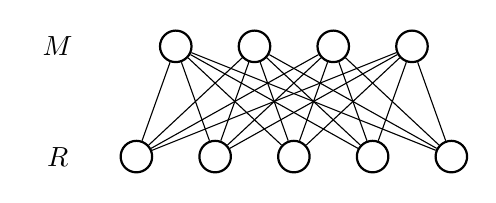
\begin{tikzpicture}[draw=black!100,scale=1.0]
 	\def \rowtwoht{1.4cm}
 	\def \rowoneht{0.0cm}
 	\tikzstyle{m-node}=[circle,draw=black!100,thick,inner sep=0pt,minimum size=4mm]
 	\tikzstyle{r-node}=[circle,draw=black!100,thick,inner sep=0pt,minimum size=4mm]
 	\tikzstyle{annot} = [text width=1.5em, text centered]
 	\node[annot] (hidden-label) at (-0.5cm,\rowtwoht) {$M$};
 	\node[annot] (surface-label) at (-0.5cm,\rowoneht) {$R$};
 	\node[m-node] 	(m0)	at (1cm,\rowtwoht)		{};
 	\node[m-node] 	(m1)	at (2cm,\rowtwoht)		{};
 	\node[m-node] 	(m2)	at (3cm,\rowtwoht)	 	{};
 	\node[m-node] 	(m3)	at (4cm,\rowtwoht) 		{};
 	% surface layer
 	\node[r-node] 	(r0)	at (0.5cm,\rowoneht)		{};
 	\node[r-node] 	(r1)	at (1.5cm,\rowoneht)		{};
 	\node[r-node] 	(r2)	at (2.5cm,\rowoneht)	 	{};
 	\node[r-node] 	(r3)	at (3.5cm,\rowoneht) 		{};
 	\node[r-node] 	(r4) 	at (4.5cm,\rowoneht)   		{};
 	%\node[r-node] 	(r5) 	at (6.5cm,\rowoneht)   		{};
 	\path (r0)	edge	node	{}	(m0)
		(r0)	edge	node	{}	(m1)
		(r0)	edge	node	{}	(m2)
		(r0)	edge	node	{}	(m3)

		(r1)	edge	node	{}	(m0)
		(r1)	edge	node	{}	(m1)
		(r1)	edge	node	{}	(m2)
		(r1)	edge	node	{}	(m3)

		(r2)	edge	node	{}	(m0)
		(r2)	edge	node	{}	(m1)
		(r2)	edge	node	{}	(m2)
		(r2)	edge	node	{}	(m3)
						
		(r3)	edge	node	{}	(m0)
		(r3)	edge	node	{}	(m1)
		(r3)	edge	node	{}	(m2)
		(r3)	edge	node	{}	(m3)

		(r4)	edge	node	{}	(m0)
		(r4)	edge	node	{}	(m1)
		(r4)	edge	node	{}	(m2)
		(r4)	edge	node	{}	(m3);
 		%(m3)	edge	node	{}	(r5);		
 \end{tikzpicture}
 \end{center}
 \caption{Bipartite graph}
 %. Neither layer contains sequential dependencies; every unit is independent within its own layer. Each hidden unit is thus free to cause any combination of observed units.}
 \label{fig:bipartite}
 \end{figure}


%Now, an MCMM, as it turns out, is a special case of a bipartite graph. Indeed,
%fig.~\ref{fig:bipartite} could itself be a simple MCMM. %precisely the architecture of an MCMM.
%%To sum up, bipartite graphs possess the properties nonlinerarity and nonsequentiality. 
%Because MCMMs are bipartite graphs, and bipartite graphs are both nonlinear and nonsequential, 
%MCMMs must themselves be nonlinear and nonsequential, which makes MCMMs well-suited for modeling
%non-concatenative morphology.

As it turns out, a bipartite graph suffices
%we do not need many partitions 
to capture the essential properties of McCarthy's autosegmental
framework,
% (fig.~\ref{subfig:nonlinear}). 
for a bipartite graph meets the two criteria stated in
(\ref{ex:criteria}).  We can reformulate the morpheme tiers and the
segmental tier in fig.~\ref{subfig:nonlinear} as the sets $M$ and
$R$, respectively, in fig.~\ref{fig:bipartite}---disjoint
by the definition of \emph{bipartite}. This satisfies the first
criterion. For the second, each node in $M$ represents a morpheme (or
morpheme tier), and, by the definition of \emph{bipartite}, the nodes
within $M$ are independent and thus orthogonal.

An MCMM (section~\ref{sec:mcmm}) is well-suited for the learning of
non-concatenative morphology because it is bipartite graph. It has two
\emph{layers} (equivalently, sets) of nodes, a hidden layer and a
surface layer---corresponding, respectively, to $M$ and $R$ in
fig.~\ref{fig:bipartite}. There are no intra-layer connections in an
MCMM, only connections between layers.
%, as in any bipartite graph.

We will henceforth refer to an MCMM's two partitions of nodes as
\emph{vectors} of nodes and will use matrix and vector notation to
describe the components of an MCMM:
%. That is, we will use
uppercase boldface letters refer to matrices, %(e.g., $\mathbf{M}$),
lowercase boldface letters refer to vectors,
% and matrix rows or columns, 
%(e.g., $\mathbf{m}_i$),
and italicized lowercase letters refer to the individual elements
of vectors/matrices. % (e.g., $m_{ik}$).
For example, $m_{i,k}$ is the $k^{\text{th}}$ element in the vector
$\mathbf{m}_i$, which is the $i^{\text{th}}$ row in the $I \times K$ matrix
$\mathbf{M}$. Thus, we will henceforth write the $M$ and $R$ in
fig.~\ref{fig:bipartite} as $\mathbf{m}$ and $\mathbf{r}$,
respectively (or $\mathbf{m}_i$ and $\mathbf{r}_i$, where $i$ is the
index of the $i^{\text{th}}$ word).


\chapter{The Multiple Cause Mixture Model}

\section{Architecture}
\label{ch4:sec:Architecture}
An MCMM is a graphical model consisting of two layers of nodes (or units): a layer of surface units 
and a layer of hidden, 
or causal, units. 
This is illustrated in fig.~\ref{fig:mcmm}, where $\mathbf{m}$ is the vector of hidden units, and $\mathbf{r}$ the vector of (reconstructed) surface units.
The hidden units are connected to surface units by a matrix of weights $\mathbf{C}$. 
Each individual arc $c_{j,k}$ has a value in $[0,1]$ that represents the weight on the connection between
$m_k$ and $r_j$.
Each node, i.e., each hidden unit and each surface unit, has an activity value in $[0,1]$ that
%Each hidden unit has an activity value in $[0,1]$ 
indicates whether it is \textsc{on} (active) or \textsc{off} (inactive).
The activity of $r_j$ is determined by a \emph{mixing function}, which takes as inputs the hidden-unit activities $\mathbf{m}$ and their respective weights $\mathbf{c}_j$
(section~\ref{sec:mixing-function}).

%Both hidden nodes and surface nodes have activity values, i.e., values in $[0,1]$ that
%indicate whether a node is \textsc{on} (active) or \textsc{off} (inactive). Each surface-node activity 
%is a function of the hidden-node activities and the weights that connect the hidden nodes to the surface node in question.

%Each surface node is either \textsc{on} (active) or \textsc{off} (inactive) depending 
%on the hidden-node activities and
%the weights connecting hidden nodes to surface nodes. 

%\subsection{Architecture}
%\label{subsec:architecture}

An MCMM can be viewed as a variant of the classical autoencoder
network \citep{dayan-and-zemel:95}, a type of neural network used for
unsupervised learning.  In autoencoders, a hidden layer is forced to
learn a compression scheme, i.e., a lower-dimensional encoding, for
a dataset.
 
%MCMMs are called \emph{Multiple Cause} Mixture Models because more
%than one hidden unit can take part in the activation of a surface
%unit.  
%This is illustrated in figure \ref{fig:mcmm}, where the nodes
%$\mathbf{m}$ are the hidden units, and $\mathbf{r}$ is the (reconstructed) surface
%vector.
%Each arc $c_{j,k}$ represents the weight on the connection between
%$m_k$ and $r_j$.
%The activity of $r_j$ is determined by a mixing function 
%(section~\ref{sec:mixing-function}).

\begin{figure*}[htb]
\begin{center}
\small
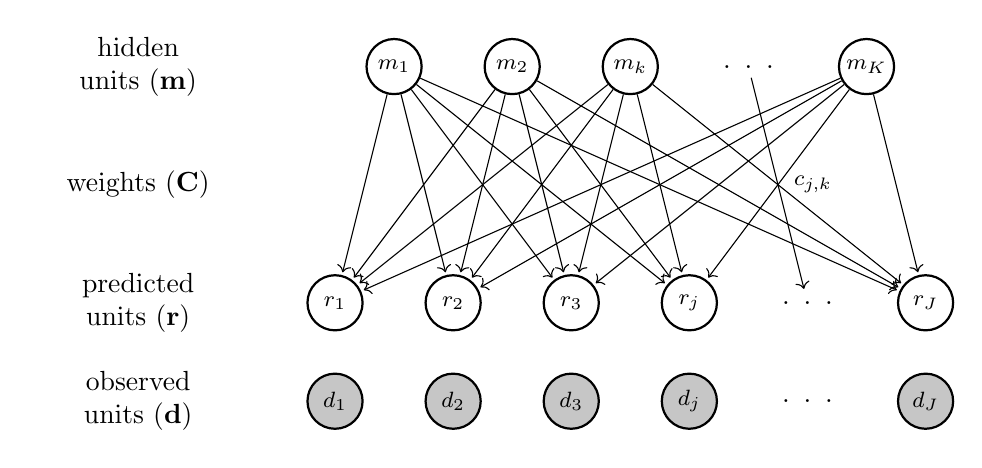
\begin{tikzpicture}[shorten >=1pt,->,draw=black!100]
	\def \rowtwoht{4.25cm}
	\def \weightlevel{2.75cm}
	\def \rowoneht{1.25cm}
	\def \basement{0cm}
	\tikzstyle{m-node}=[circle,draw=black!100,thick,inner sep=0pt,minimum size=7mm]
	\tikzstyle{r-node}=[circle,draw=black!100,thick,inner sep=0pt,minimum size=7mm]
	\tikzstyle{d-node}=[circle,draw=black!100,fill=gray!45,thick,inner sep=0pt,minimum size=7mm]
	\tikzstyle{dots}=[text width=5ex, text centered]
	\tikzstyle{annot}=[text width=17ex, text centered]
	% labels
	\node[annot] (hidden-layer) at (0cm,\rowtwoht) {hidden units ($\mathbf{m}$)};
	\node[annot] (weights) at (0cm,\weightlevel) {weights ($\mathbf{C}$)};
	\node[annot] (r-layer) at (0cm,\rowoneht) {predicted units ($\mathbf{r}$)};
	\node[annot] (d-layer) at (0cm,\basement) {observed units ($\mathbf{d}$)};
	
	\node[dots] 	(m3)	at (7.75cm,\rowtwoht)	 	{. . .};
	\node[dots] 	(r4) 	at (8.5cm,\rowoneht)   		{. . .};
	\node[dots] 	(d4) 	at (8.5cm,\basement)   		{. . .};
	
	\footnotesize
	% hidden layer
	\node[m-node] 	(m0)	at (3.25cm,\rowtwoht)		{$m_1$};
	\node[m-node] 	(m1)	at (4.75cm,\rowtwoht)		{$m_2$};
	\node[m-node] 	(m2)	at (6.25cm,\rowtwoht)	 	{$m_k$};
	\node[m-node] 	(m4)	at (9.25cm,\rowtwoht)	 	{$m_K$};
	
	% reconstructed vector
	\node[r-node] 	(r0)	at (2.5cm,\rowoneht)		{$r_1$};
	\node[r-node] 	(r1)	at (4cm,\rowoneht)		{$r_2$};
	\node[r-node] 	(r2)	at (5.5cm,\rowoneht)	 	{$r_3$};
	\node[r-node] 	(r3)	at (7cm,\rowoneht) 		{$r_j$};
	\node[r-node] 	(r5) 	at (10cm,\rowoneht)   		{$r_J$};
	%\node[r-node] 	(r6) 	at (9.75cm,\rowoneht)   	{$r_J$};
	
	% data vector
	\node[d-node] 	(d0)	at (2.5cm,\basement)		{$d_1$};
	\node[d-node] 	(d1)	at (4cm,\basement)		{$d_2$};
	\node[d-node] 	(d2)	at (5.5cm,\basement)	 	{$d_3$};
	\node[d-node] 	(d3)	at (7cm,\basement) 		{$d_j$};
	\node[d-node] 	(d5) 	at (10cm,\basement)   		{$d_J$};
	%\node[d-node] 	(d6) 	at (9.75cm,\basement)   	{$d_J$};
	
	\path 
		(m0)	edge	node	{}	(r0)
		(m0)	edge	node	{}	(r1)
		(m0)	edge	node	{}	(r2)
		(m0)	edge	node	{}	(r3)
		(m0)	edge	node	{}	(r5)
		(m1)	edge	node	{}	(r0)
		(m1)	edge	node	{}	(r1)
		(m1)	edge	node	{}	(r2)
		(m1)	edge	node	{}	(r3)
		(m1)	edge	node	{}	(r5)
		(m2)	edge	node	{}	(r0)
		(m2)	edge	node	{}	(r1)
		(m2)	edge	node	{}	(r2)
		(m2)	edge	node	{}	(r3)
		(m2)	edge	node	{}	(r5)
		(m3)	edge	node[right=1mm]	{$c_{j,k}$}	(r4)
		%	
		(m4)	edge	node	{}	(r0)
		(m4)	edge	node	{}	(r1)
		(m4)	edge	node	{}	(r2)
		(m4)	edge	node	{}	(r3)
		(m4)	edge	node	{}	(r5);
		
\end{tikzpicture}
\end{center}
\caption{Architecture of a Multiple Cause Mixture Model (MCMM)} 
\label{fig:mcmm}
\end{figure*}

%The MCMM learns by comparing the reconstructed vector $\mathbf{r}_i$ 
%to its corresponding original datapoint $\mathbf{d}_i$. The discrepancy between
%the two is quantified by an \emph{objective function}. 
%If there is a discrepancy, the values of the nodes in
%$\mathbf{m}_i$ as well as the weights $\mathbf{C}$ are adjusted 
%in order to reduce the discrepancy as much as possible.
%See section~\ref{sec:mcmm-learning} for more on the learning process.

%Suppose data points $\mathbf{d}_u$ and $\mathbf{d}_v$ have some features in common.
%Then, as the MCMM tries to reconstruct them in $\mathbf{r}_u$ and $\mathbf{r}_v$, respectively,
%similarities will emerge between their respective hidden-layer vectors $\mathbf{m}_u$ and $\mathbf{m}_v$.
%In particular, the vectors $\mathbf{m}_u$ and
%$\mathbf{m}_v$ should come to share at least one active node, i.e., at least
%one $k \in K$ such that $m_{u,k} = 1$ and $m_{v,k} = 1$.
%This can serve as a basis for clustering;
%i.e., $m_{i,k}$ indicates whether $\mathbf{d}_i$ is a member of cluster $k$.
		
\section{Mixing Function}
\label{ch4:sec:mixing-function}

The mapping between the layer of hidden nodes $\mathbf{m}$ 
and the layer of surface nodes $\mathbf{r}$ is governed by a 
\emph{mixing function}, which is essentially
a voting rule \citep{saund:94}; it maps from a set of (weighted)
input ``votes'' to a single output decision.  The output decision is 
an activity value for a particular surface-layer node. We will call the input votes
\emph{causes}. 

Each cause is a product of the form $m_{i,k} c_{j,k}$ for $k \in K$.
There are thus a total of $K$ distinct causes for a given surface node $r_{i,j}$. 
If the cause $m_{i,h} c_{j,h}$, where $h \in K$, is equal to $1$ or surpasses some
threshold, then $m_{i,h} c_{j,h}$ is an \emph{active cause}.
%The input votes, are the activities of the hidden nodes,
%i.e., the $K$-length vector $\mathbf{m}_i$,
%coupled with their respective weights, i.e., the $K$-length vector 
%$\mathbf{c}_j$. 
Any differentiable function
that maps from the vector pair $(\mathbf{m}_i, \mathbf{c}_j)$ 
to an activity value for $r_{i,j}$ can in theory serve as a mixing function. 
There are thus an infinite number of theoretically possible mixing functions.

%Following \cite{saund:94}, we use the 
%There are perhaps an infinite number of possible mixing functions. 
%Any function that maps from a set of votes 
%(and their respective weights) to a single output decision will suffice.
One possibility is the \textbf{Noisy-OR} function:
 \begin{equation}\label{eq:noisy-or}
  r_{i,j} = 1 - \prod\limits_{k} (1 - m_{i,k} c_{j,k})
 \end{equation}
% We will call the inputs to the Noisy-OR function \emph{causes}. Each cause is a product of the form $m_{i,k} c_{j,k}$. 
 The Noisy-OR function acts as a kind of \textit{OR} gate, or, to put it another way, an``at-least-one" gate. That is, the surface node $r_{i,j}$ is $1$ as long as \emph{at least one} cause is active.
 % (i.e., $m_{i,k} c_{j,k} = 1$ for at least one $k$ in $K$). 
 If two or more causes are active,
%$1$ (or $\ge$ than a threshold), 
$r_{i,j}$ is still going to be $1$. The output of Noisy-OR does not change as the number of active causes change, as long as there is at least one active cause.

Another possible mixing function is the \textbf{sigmoidal weighted sum}, the composition of the sigmoid function $S$ and the function $t_{i,j}$, which computes a weighted sum, i.e., the inner product of the cluster-activity vector $\mathbf{m}_i$ and the weight vector $\mathbf{c}_j$:

	\begin{align} %\label{eq:sigws}
	\label{eq:sig}
	r_{i,j} = S(t_{i,j}) &= \frac{1}{1 + e^{-t_{i,j}}} \quad %\\   %\qquad \text{where} \quad
	%\label{eq:ws}
	\text{where} \quad t_{i,j} = \sum_k m_{i,k} c_{j,k}
	\end{align}
This is the mixing (or activation) function that is typically used in classical autoencoders. 
Whereas the output of Noisy-OR is independent of the number of active causes (as long as there is at least one), the output of \eqref{eq:sig} DOES change with the number of active causes: The value $t_{i,j} = \sum_k m_{i,k} c_{j,k}$ is clearly going to increase as the number of active clusters increases.
%(i.e., products of the form $m_{i,k} c_{j,k}$ that equal $1$ or are greater than some threshold) 
As $t_{i,j}$ increases, $S(t_{i,j})$ will get closer to $1$; as %it
$t_{i,j}$ 
decreases, $S(t_{i,j})$ will get closer to $0$.


\section{Learning}
\label{ch4:sec:learning}
%\label{autoencoder-learning}

% A data compression scheme is useful only to the extent that it allows
% for the recovery of the source data from the compressed
% representations. In autoencoder terms, this means that 

%The reconstruction layer attempts to
%decode the hidden layer's representations and
In both the classical autoencoder and the MCMM, learning occurs as a
result of the algorithm's search for an optimal valuation of key variables (e.g., weights), 
i.e., a valuation that minimizes %or maximizes an the
%\emph{reconstruction error} $E$, 
the discrepancy between
reconstructed and original data points.  The search is conducted
via %some method of 
numerical optimization; we use the nonlinear conjugate gradient method.
%gradient-based technique, e.g., gradient descent or
%the conjugate gradient method.
%
Our objective function is a simple error function, namely the
normalized sum of squares error:
\begin{equation}
E = \frac{1}{I \times J} \sum_{i} \sum_{j} {(r_{i,j} - d_{i,j})}^2
\end{equation}
 where $I \times J$ is the total number of features in the dataset.
The MCMM's task is to minimize this function by adjusting the
 values in $\mathbf{M}$ and $\mathbf{C}$, where
 %$I \times $ matrix $\mathbf{M}$ and the $J \times K$ matrix $\mathbf{C}$.
$\mathbf{M}$ is the $I \times K$ matrix that
% of dimensions $I \times K$,
encodes each data point's cluster-activity vector, 
and $\mathbf{C}$ is the $J \times K$ matrix that
%, of dimensions $J \times K$, 
encodes the weights between $\mathbf{m}_i$ and $\mathbf{r}_i$ for every $i \in I$ (see fig.~\ref{fig:example}). 
%$\mathbf{C}$ can also be interpreted as encoding the cluster centroids 
%(the clusters' ``average'' data points).
%Each column in $\mathbf{C}$ is in effect a feature vector; the $k^{\text{th}}$ column is 
%the $k^{\text{th}}$ cluster's average feature vector.
% \begin{align*}
% 	% E &= \frac{1}{I} \sum_{i} e_{i} \\
% 	% e_{i} &= \frac{1}{J} \sum_{j} {(r_{i,j} - d_{i,j})}^2
% 	E &= \frac{1}{I \times J} \sum_{i} \sum_{j} {(r_{i,j} - d_{i,j})}^2
% \end{align*}
% %\marginpar{Rationale for normalized SSE?} 
% which is minimized.
% rather than maximized.  


%; our techniques are described in section~\ref{subsec:objfunc}.
% There are a number of possibilities regarding the particular error
% function and gradient-based technique. We describe our choices in
% section~\ref{subsec:objfunc}.
% Any information loss in the compression will result in reconstructed
% vectors that differ from the original data points.  This is called
%the \emph{reconstruction error} is measured by some error function
%$err$, such as the
%%.  A typical error function is 
%the sum of squared error ($err_i = \sum_{j}{(d_{i,j} -
%  r_{i,j})}^2$). The global reconstruction error $E$, for the whole
%dataset, is the sum of all $err_i$.
%% over $i \in I$.
%%
%To discover a compression scheme with a minimal $E$, autoencoders
%use gradient-based search techniques, e.g., gradient descent or the
%conjugate gradient method.  We describe our error function in
%section~\ref{subsec:objfunc}.

% The autoencoder's goal is to discover a compression scheme that causes a minimal $E$, 
% and since $E$ is ultimately a function of $\mathbf{A}$ and $\mathbf{B}$, 
% this task reduces to finding the valuations for $\mathbf{A}$ and $\mathbf{B}$ that minimize $E(\mathbf{A},\mathbf{B}$). To this end, autoencoders use gradient-based search techniques, e.g., gradient descent or the conjugate gradient method. In the remainder of this section, we provide a very general description of an autoencoder's weight updating process. The details, especially the specific form of the weight-update function, depend on the particular gradient-based technique used. 

% Taking as input the data points $\mathbf{d}_i \in \mathbf{D}$, the network yields a reconstructed vector $\mathbf{r}_i$ for each individual $\mathbf{d}_i$. Because $\mathbf{D}$ contains $I$ data points, one epoch (i.e., one cycle through the dataset) is complete after $I$ iterations, whereupon ${E}(\mathbf{A}, \mathbf{B})$ is calculated, and each weight in $\mathbf{A}$ and $\mathbf{B}$ is adjusted in a way that furthers the descent of $E$ toward a minimum. 
% In particular, the algorithm adds to each 
% $b_{k,j} \in \mathbf{B}$ a quantity proportional to the negative gradient of 
% $E$ at $b_{k,j}$, or $-\frac{\partial E}{\partial b_{k,j}}$. 
% It similarly adds to each $a_{j,k} \in \mathbf{A}$
% a quantity proportional to the negative gradient of $E$ at $a_{j,k}$,
% or $-\frac{\partial E}{\partial a_{j,k}}$.
% These weight updates serve to improve the network's compression model, so that each successive epoch yields a smaller reconstruction error than the preceding epoch.
% The succession of epochs continues until $E$ falls below some small predesignated value.


% \subsection{The MCMM as an autoencoder variant}
% \label{subsec:mcmm-variant}

%\subsubsection{Architecture}
% Like the classical autoencoder, the MCMM has a hidden layer $\mathbf{m}$ and a reconstruction layer $\mathbf{r}$, as illustrated in figure \ref{fig:mcmm}. 
% However, the MCMM does not have an explicit
% data (or input) layer corresponding to the classical autoencoder's $\mathbf{d}$.
% Because the MCMM has only a two layers of nodes instead of three, it needs only a single layer of connecting weights, namely the weight matrix $\mathbf{C}$. This is a $J \times K$ matrix,
% since there are $K$ nodes in $\mathbf{m}$ and $J$ nodes in $\mathbf{r}$,
% and every $m_k$ must be linked to every $r_j$.

%\subsubsection{Mixing Function}
% MCMMs are distinguished by their propensity for learning hidden-unit activations and weight configurations that have clear interpretations.

% In the classical autoencoder, the activity $\phi(net)$ of any node $y$ is a
% function of its net raw input $net_y$, which is the weighted sum of $y$'s
% individual input signals (see \eqref{weighted-sum}). 
% The logistic sigmoid function $\phi$ then scales ${net}_y$ so that it falls within $[0,1]$.

% \begin{align*}
% r_{j} &= \sigma({net}_j) \\
% &= \sigma\big(\sum_k b_{k,j} \cdot m_k \big) \\
% &= \sigma \bigg(\sum_k b_{k,j} \cdot \sigma \big({net}_k \big) \bigg) \\
% &= \sigma \bigg(\sum_k b_{k,j} \cdot \sigma \big(\sum_j a_{j,k} \cdot d_j \big) \bigg) \\
% \end{align*}
% The activity of any given reconstruction node $r_j$ depends not only on the weights $\mathbf{B}$, but also on the weights $\mathbf{A}$.
% Moreover, $\mathbf{A}$ and $\mathbf{B}$ may differ.
% When $\mathbf{A} \ne \mathbf{B}$, the $\mathbf{B}$ weights can counteract the effects of the $\mathbf{A}$ weights, giving rise to unexpected activities among the $\mathbf{m}$ units and obscuring the  
% relationships between the $\mathbf{m}$ units and the $\mathbf{r}$ units.

% The MCMM, in contrast, is designed with the express purpose of providing a coherent causal explanation for regularities in surface data.
% What makes this possible?
% \begin{itemize} 
% \item \textit{Binary activities and weights.} Both the weights and the hidden unit activities are constrained to stay in $[0,1]$. At convergence, moreover, all values---both weights and hidden activities---should be either $0$ or $1$. \textit{Why is this important?} Binary values, i.e., \textsc{true} and \textsc{false}, have clear interpretations.
% \item \textit{Single layer of weights.} An MCMM has only one layer of weights. \textit{Why is this important?} The activities of the hidden units are manipulated directly in response to the reconstruction error.
% \item 
% \textit{How so?} In the classical autoencoder, the terms $m_kc_{j,k}, k \in K$ are combined linearly prior to sigmoid squashing. But MCMMs employ mixing functions such that the combination of these terms is nonlinear from the start. \textit{Why does this matter?} This ``total" nonlinearity encourages (?) weights to converge toward discrete values. The ultimate decision is then based on multiple discrete, either-or votes.
% \textit{Why, then, is clipping necessary?}
% \end{itemize}

% The classical autoencoder's activation function $\sigma({net}_y)$ is one possible mixing function,
% for it indeed takes the $K$ distinct input signals to node $y$ and yields a single activity value.
% However, as Saund points out, $\sigma({net}_y)$ is not well suited to the purpose of coherently distinguishing causes from non-causes. This is because $net_y$ is additive rather than multiplicative. Noisy-or is multiplicative:
% \begin{align*}
% r_{j} &= 1 - (1 - m_0c_{0,j}) \times (1 - m_1c_{1,j}) \times (1 - m_2c_{2,j}) \\
% &= 1 - (1 - 0) \times (1 - 0) \times (1 - 1) \\ 
% &= 1 - 1 \times 1 \times 0 \\
% &= 1
% \end{align*}
% As long as at least one $m_kc_{j,k} = 1$ (where $k = 0,1,\dots,K$), $r_{j}$ will be active,
% and $r_{j} = 0$ only if all products $m_kc_{j,k}$ are zero.
% Notice that $m_kc_{j,k} = 1$ only if both $m_k = 1$ and $c_{j,k} = 1$.
% On the other hand, with sigmoid squashing, $\sigma({net}_j)$ is never truly zero; it just gets infinitely close to zero.
% And $\sigma({net}_j)$ will be close to $1$ as long as ${net}_j = \sum_K m_k c_{j,k}$ is sufficiently large. 
% There are an infinite number of valuations for $\mathbf{m}$ and $\mathbf{c}_{j}$ that could give rise to a sufficiently large ${net}_j$.

% The function ${net}$ is an example of a linear mixing function. However, the autoencoder's mixing function
% is made nonlinear by $\phi({net}_y)$, which ``squashes" $net_y$ to fall within $[0,1]$.

%\subsubsection{Learning}
%\label{mcmm-learning}

%\paragraph{MCMM}

%\marginpar{MD: In fig.~\ref{fig:example}, we use $\mathbf{M}$, but
%  in previous figures we use $\mathbf{m}$.  Also, why is it sometimes
%  $\mathbf{m_k}$ and sometimes $\mathbf{m_{i,k}}$?  ($i$ refers to the
%  $i^{\text{th}}$ word?)}

The MCMM's learning process is similar to Expectation Maximization
(EM) in that at any given time it holds one set of variables 
fixed while optimizing the other set. We thus have two functions, \textsc{Optimize-M}
and \textsc{Optimize-C}, which take turns optimizing their respective matrices.
% However, if the algorithm is to optimize $\mathbf{M}$, it must first
% know $\mathbf{C}$, and vice versa.  Therefore, the algorithm can only
% focus on matrix at time, optimizing the one while holding the other
% fixed.
% The learning process consists of two distinct optimization
% functions:
%, \textsc{Optimize-M} and \textsc{Optimize-C}.
%\begin{description}
%\item[
% \textsc{Optimize-M} holds $\mathbf{C}$ fixed in order to optimize the
% cluster activity vectors in $\mathbf{M}$, while \textsc{Optimize-C}
% holds $\mathbf{M}$ fixed in order to optimize the cluster centroids in
% $\mathbf{C}$.
%\end{description}

The function \textsc{Optimize-M} visits each of the $I$ cluster-activity vectors $\mathbf{m}_i$ in
$\mathbf{M}$, optimizing each one separately.
%, one at a time.
%in $\mathbf{M}$, 
For each $\mathbf{m}_i$, \textsc{Optimize-M} enters an optimization 
loop over its $K$ components, adjusting each 
$m_{i,k}$ by a
quantity proportional to the negative gradient of $E$ at $m_{i,k}$. \marginpar{How is this proportion determined?}
%(details omitted for space reasons). 
This loop repeats until $E$
ceases to decrease significantly,
%with respect to $m_{i,k}$,
%(i.e., $E$ stops decreasing significantly),
whereupon \textsc{Optimize-M} proceeds to the next $\mathbf{m}_i$.  
% \textsc{Optimize-M} is thus a succession of $I$ optimization loops, one
% loop for each cluster activity vector $\mathbf{m}_i$. 
%(i.e., for each of the $i$ data points).

The function \textsc{Optimize-C} consists of a single optimization loop over the 
entire matrix
$\mathbf{C}$. Each %component 
$c_{j,k}$ is adjusted by a quantity
proportional to the negative gradient of $E$ at $c_{j,k}$.
%, or $-\frac{\partial E}{\partial c_{j,k}}$.
%(in the case of gradient descent).  
%Since $E$ is simply
%$\sum_i e_i$, i.e., the sum of the errors of the individual data-point
%reconstructions, $-\frac{\partial E}{\partial c_{j,k}} = -\sum_i
%\frac{\partial e_i}{\partial c_{j,k}}$.  Thus, the adjustment to each
%$c_{j,k}$ takes into account the error of each reconstructed vector
%$\mathbf{r}_i$ in $\mathbf{R}$. However,
Unlike \textsc{Optimize-M}, which comprises $I$ separate optimization
loops, \textsc{Optimize-C} consists of just one, 
%optimizing the $\mathbf{C}$ matrix as a whole.  
When each of its $J \times K$
components has been adjusted, one round of updates to $\mathbf{C}$ is
complete.  $E$ is reassessed only between completed rounds of
updates. If the change in $E$ remains significant, another round begins.  

% \marginpar{MD: I wasn't sure whether I should include
%   somehting about Armijo conditions. TM: We probably don't have to go into that.}
%  (We use a non-linear conjugate
%gradient method for the update rules, but, again, details are omitted
%for space reasons. 

Both \textsc{Optimize-M} and \textsc{Optimize-C} are enclosed within 
an ``alternation loop" 
that alternates between the two functions, holding $\mathbf{C}$ fixed
during \textsc{Optimize-M}, and vice versa.
%$\mathbf{M}$ fixed during \textsc{Optimize-C}. 
This alternation continues until $E$ cannot be decreased further. At
this point, an ``outer loop''
%(containing the alternating loop) 
splits the cluster which contributes the most to the error, adds one
to the cluster count $K$, and restarts the alternation loop. The outer loop
repeats until it reaches an overall stopping criterion, e.g., $E = 0$.
%; otherwise, the function terminates.
 \subsection{Bound Constrained Optimization}
The optimization task is subject to the constraint %$0 le m_{i,k} ge 1$
that no value in $\mathbf{M}$ or $\mathbf{C}$ may exceed 1 or fall below 0. In other words,
it is a task of bound constrained optimization. Thus, whenever a value in either $\mathbf{M}$ or $\mathbf{C}$ is about
to fall below 0, it is set to 0. Likewise, whenever a value is about to exceed 1, it is set to 1
\citep{ni:yuan:1997}.
 %It repeatedly iterates over the $J \times K$ components of $\mathbf{C}$, stopping only when it finds a local minimum of $E$ is
  
%What is the inner loop and what is the outer loop?
%There are actually two inner loops: Opt-M is immediately followed by Opt-C. These two are encapsulated within a larger outer loop.
%What is the stopping criterion for the inner loop? What happens when this criterion is met?
%What is the stopping criterion for the outer loop?
%Cluster Splitting. Where does this enter the narrative?
%At this point, the algorithm then finds the worst cluster among the currently existing clusters and splits it, thereby increasing the cluster count $K$ by one.

\subsection{A Simple MCMM Example}
\label{subsec:example}

Fig.~\ref{fig:example} shows an example of an MCMM for two data points (i.e., $I = 2$).
% is given in fig.~\ref{fig:example}, for $I=2$,
%i.e., 2 data points. , each with 3 features.
%
%Together, 
The hidden cluster activities $\mathbf{M}$, the weights $\mathbf{C}$,
and the mixing function $r$ constitute a model that reproduces the
observed data points $\mathbf{D}$.
%
%\marginpar{MD: I don't quite understand the ``center vector''
  %statement}
%
The nodes $m_{i,k}$ represent cluster activities; if $m_{1,2} = 1$,
for instance, the second cluster is active for $\mathbf{d}_1$ (i.e.,
$\mathbf{d}_1$ is a member of cluster 2).
%
Note that the $J \times K$ weight matrix $\mathbf{C}$ is the same for
all data points, and
%
% For each data point, the arcs emanating from cluster
% 1 and cluster 2 represent the components of $\mathbf{C}$'s first and
% second rows, respectively. The $k$th row in $\mathbf{C}$ is thus
% uniquely associated with the $k$th cluster. Moreover, 
%
the $k^{\text{th}}$ row in $\mathbf{C}$ can be seen as the $k^{\text{th}}$
cluster's ``average" vector: the $j^{\text{th}}$ component in
$\mathbf{c}_k$ is 1 only if all data points in cluster $k$ have
1 at feature $j$.
%the $k^{\text{th}}$ row of $\mathbf{C}$ is in effect
%the center vector of the $k^{\text{th}}$ hidden cluster.
%
%In the figure, 

%\begin{figure}[htb!]
%\usetikzlibrary{positioning}
%%\begin{minipage}{.3\textwidth}
%\begin{center}
%%\subfigure[Learning in Progress]{
%\begin{tikzpicture}[shorten >=1pt,->,draw=black!100, scale=0.85]
%	\footnotesize
%%	\def \attic{5.95cm}
%%	\def \rowtwoht{5.4cm}
%%	\def \weightlevel{3.9cm}
%%	\def \rowoneht{2.4cm}
%%	\def \basement{1.8cm}
%%	\def \data{1cm}
%%	\def \china{0cm}
%
%	\def \attic{5.4cm}
%	\def \rowtwoht{4.8cm}
%	\def \weightlevel{3.6cm}
%	\def \rowoneht{2.4cm}
%	\def \basement{1.8cm}
%	\def \data{1cm}
%	\def \china{0cm}
%		
%	\tikzstyle{m-node}=[circle,draw=black!100,thick,inner sep=0pt,minimum size=6mm]
%	\tikzstyle{r-node}=[circle,draw=black!100,thick,inner sep=0pt,minimum size=6mm]
%	\tikzstyle{d-node}=[circle,draw=black!100,fill=gray!45,thick,inner sep=0pt,minimum size=6mm]
%	%\tikzstyle{dots}=[text width=5ex, text centered]
%	\tikzstyle{annot}=[text width=2.5em]
%	% labels
%	\tikzstyle{label}=[text width=2.5em, text centered]
%	\tikzstyle{formula}=[text width=30em, text centered]
%	
%	\scriptsize
%	\node[annot] (hidden-layer) at (0cm,\rowtwoht) {$\mathbf{M}_{(i,k)}$};
%	\node[annot] (weights) at (0cm,\weightlevel) {$\mathbf{C}_{(j,k)}$};
%	\node[annot] (r-layer) at (0cm,\rowoneht) {$\mathbf{R}_{(i,j)}$};
%	
%	% hidden layer
%	\scriptsize
%	\node[m-node] 	(ma00)	at (1.45cm,\rowtwoht)		{$.2$};
%	\node[m-node] 	(ma01)	at (3.35cm,\rowtwoht)		{$.9$};
%	\node[m-node] 	(ma10)	at (5.55cm,\rowtwoht) 	{$.8$};
%	\node[m-node] 	(ma11)	at (7.45cm,\rowtwoht)	 	{$.1$};
%	% \node[m-node] 	(m20)	at (9.65cm,\rowtwoht) 	{$.8$};
%	% \node[m-node] 	(m21)	at (11.55cm,\rowtwoht)	 	{$.9$};
%	
%	%\footnotesize
%	\node[label]	(ml00) 	at (1.45cm,\attic)		{$m_{1,1}$}; %1.75 -> 1.45
%	\node[label]	(ml01) 	at (3.35cm,\attic)		{$m_{1,2}$}; %3.05 -> 3.35
%	\node[label] 	(ml10)	at (5.55cm,\attic) 	{$m_{2,1}$};     %5.85 -> 5.55
%	\node[label] 	(ml11)	at (7.45cm,\attic)	 	{$m_{2,2}$}; %7.15 -> 7.45
%	% \node[label] 	(ml20)	at (9.65cm,\attic) 	{$m_{3,1}$};     %9.95 -> 9.65
%	% \node[label] 	(ml21)	at (11.55cm,\attic)	 	{$m_{3,2}$}; %11.25 -> 11.55
%	
%	\scriptsize
%	\node[r-node] 	(ra00)	at (1.1cm,\rowoneht)		{$.24$};
%	\node[r-node] 	(ra01)	at (2.4cm,\rowoneht)		{$.81$};
%	\node[r-node] 	(ra02)	at (3.7cm,\rowoneht)	 	{$.23$};
%	
%	\node[r-node] 	(ra10)	at (5.2cm,\rowoneht) 		{$.68$};
%	\node[r-node] 	(ra11) 	at (6.5cm,\rowoneht)   	{$.16$};
%	\node[r-node] 	(ra12)	at (7.8cm,\rowoneht)		{$.76$};
%	
%	% \node[r-node] 	(r20) 	at (9.3cm,\rowoneht)  		{$.71$};
%	% \node[r-node] 	(r21)	at (10.6cm,\rowoneht) 		{$.83$};
%	% \node[r-node] 	(r22) 	at (11.9cm,\rowoneht)   	{$.77$};
%	
%	\node[label] 	(rl00)	at (1.1cm,\basement)		{$r_{1,1}$};
%	\node[label] 	(rl01)	at (2.4cm,\basement)		{$r_{1,2}$};
%	\node[label] 	(rl02)	at (3.7cm,\basement)	 	{$r_{1,3}$};
%	
%	\node[label] 	(rl10)	at (5.2cm,\basement) 		{$r_{2,1}$};
%	\node[label] 	(rl11) 	at (6.5cm,\basement)   	{$r_{2,2}$};
%	\node[label] 	(rl12)	at (7.8cm,\basement)		{$r_{2,3}$};
%	
%%	\node[label] 	(rl20) 	at (9.3cm,\basement)  		{$r_{3,1}$};
%%	\node[label] 	(rl21)	at (10.6cm,\basement) 		{$r_{3,2}$};
%%	\node[label] 	(rl22) 	at (11.9cm,\basement)   	{$r_{3,3}$};
%
%	\draw[-] (4.45cm, \attic+1.5mm) -- (4.45cm, \basement-1.5mm);
%%	\draw[-] (8.55cm, \attic+1.5mm) -- (8.55cm, \basement-1.5mm);
%
%	\scriptsize
%	\path
%		(ma00)	edge	node [left]	{$.85$} (ra00)
%		(ma00)	edge	node [left,xshift=-1mm,yshift=3mm]	{$.1$}	(ra01)
%		(ma00)	edge	node [left,xshift=-1mm,yshift=8mm]	{$.95$}	(ra02)
%
%		(ma01)	edge	node [right,xshift=3mm,yshift=8mm]	{$.1$}	(ra00)
%		(ma01)	edge	node [right,xshift=1mm,yshift=3mm]	{$.9$}	(ra01)
%		(ma01)	edge	node [right]	{$.05$} (ra02)
%		%
%		(ma10)	edge	node [left] {$.85$} (ra10)
%		(ma10)	edge	node [left,xshift=-1mm,yshift=3mm]	{$.1$}	(ra11)
%		(ma10)	edge	node [left,xshift=-1mm,yshift=8mm] {$.95$}	(ra12)
%		
%		(ma11)	edge	node [right,xshift=3mm,yshift=8mm]	{$.1$}	(ra10)
%		(ma11)	edge	node [right,xshift=1mm,yshift=3mm]	{$.9$}	(ra11)
%		(ma11)	edge	node [right]	{$.05$} (ra12);
%		%
		% (m20)	edge	node [left]	{$.85$}	(r20)
		% (m20)	edge	node [left,xshift=-1mm,yshift=4mm]	{$.1$}	(r21)
		% (m20)	edge	node [left,xshift=-1mm,yshift=10mm]	{$.95$} (r22)
		
		% (m21)	edge	node [right,xshift=3mm,yshift=10mm]		{$.1$}	(r20)
		% (m21)	edge	node [right,xshift=1mm,yshift=4mm]{$.9$}	(r21)
		% (m21)	edge	node [right]	{$.05$}	(r22);		
		
%\end{tikzpicture}
%\label{fig:example:fig1}
%\caption{A simple MCMM example} % showing learning in progress}
%\label{fig:example:fig1}
%\end{center}
%\end{figure}

\begin{figure}[htb!]
\usetikzlibrary{positioning}
\begin{center}
\subfigure[Observed Data]{
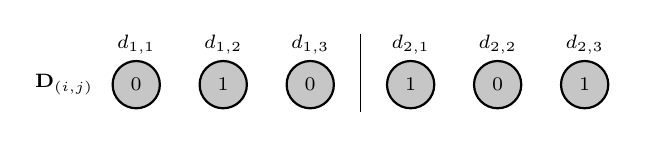
\begin{tikzpicture}[shorten >=1pt,->,draw=black!100, scale=0.85]
	\scriptsize
	\tikzstyle{label}=[text width=3em, text centered]
	\tikzstyle{annot}=[text width=2.5em]
	\tikzstyle{d-node}=[circle,draw=black!100,fill=gray!45,thick,inner sep=0pt,minimum size=6mm]
	
	\def \china{0.6cm}
	\def \data{0cm}
	
	\node[annot] (d-layer) at (0cm,\data) {$\mathbf{D}_{(i,j)}$};
	\draw[-] (4.45cm, \china+1.5mm) -- (4.45cm, \data-4.5mm);
%	\draw[-] (8.55cm, \china+1.5mm) -- (8.55cm, \data-4.5mm);
	%\draw[-] (-1cm, \china+.5cm) -- (13cm, \china+.5cm);
	%\draw[-] (-1cm, \data-.5cm) -- (13cm, \data-.5cm);
	
	\node[label] 	(dl00)	at (1.1cm,\china)		{$d_{1,1}$};
	\node[label] 	(dl01)	at (2.4cm,\china)		{$d_{1,2}$};
	\node[label] 	(dl02)	at (3.7cm,\china)	 	{$d_{1,3}$};
	
	\node[label] 	(dl10)	at (5.2cm,\china) 		{$d_{2,1}$};
	\node[label] 	(dl11) 	at (6.5cm,\china)   	{$d_{2,2}$};
	\node[label] 	(dl12)	at (7.8cm,\china)		{$d_{2,3}$};
	
	% \node[label] 	(dl20) 	at (9.3cm,\china)  		{$d_{3,1}$};
	% \node[label] 	(dl21)	at (10.6cm,\china) 		{$d_{3,2}$};
	% \node[label] 	(dl22) 	at (11.9cm,\china)   	{$d_{3,3}$};
	
	\node[d-node] 	(d00)	at (1.1cm,\data)		{$0$};
	\node[d-node] 	(d01)	at (2.4cm,\data)		{$1$};
	\node[d-node] 	(d02)	at (3.7cm,\data)		{$0$};

	\node[d-node] 	(d10)	at (5.2cm,\data)		{$1$};
	\node[d-node] 	(d11)	at (6.5cm,\data)		{$0$};
	\node[d-node] 	(d12)	at (7.8cm,\data)		{$1$};
	
	% \node[d-node] 	(d20)	at (9.3cm,\data)		{$1$};
	% \node[d-node] 	(d21)	at (10.6cm,\data)		{$1$};
	% \node[d-node] 	(d22)	at (11.9cm,\data)		{$1$};
\end{tikzpicture}
\label{fig:example:subfig0}
}
\end{center}

\usetikzlibrary{positioning}
%\begin{minipage}{.3\textwidth}
\begin{center}
\subfigure[Learning in Progress]{
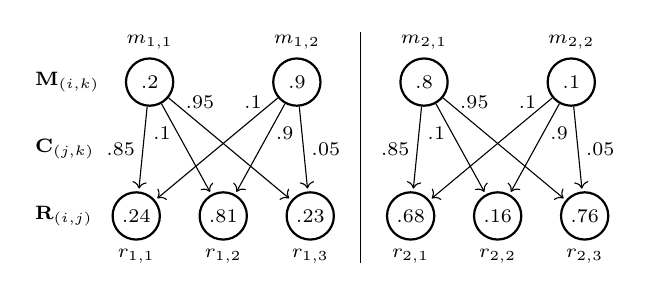
\begin{tikzpicture}[shorten >=1pt,->,draw=black!100, scale=0.85]
	\footnotesize
%	\def \attic{5.95cm}
%	\def \rowtwoht{5.4cm}
%	\def \weightlevel{3.9cm}
%	\def \rowoneht{2.4cm}
%	\def \basement{1.8cm}
%	\def \data{1cm}
%	\def \china{0cm}

	\def \attic{5cm}
	\def \rowtwoht{4.4cm}
	\def \weightlevel{3.4cm}
	\def \rowoneht{2.4cm}
	\def \basement{1.8cm}
	\def \data{1cm}
	\def \china{0cm}
		
	\tikzstyle{m-node}=[circle,draw=black!100,thick,inner sep=0pt,minimum size=6mm]
	\tikzstyle{r-node}=[circle,draw=black!100,thick,inner sep=0pt,minimum size=6mm]
	\tikzstyle{d-node}=[circle,draw=black!100,fill=gray!45,thick,inner sep=0pt,minimum size=6mm]
	%\tikzstyle{dots}=[text width=5ex, text centered]
	\tikzstyle{annot}=[text width=2.5em]
	% labels
	\tikzstyle{label}=[text width=2.5em, text centered]
	\tikzstyle{formula}=[text width=30em, text centered]
	
	\scriptsize
	\node[annot] (hidden-layer) at (0cm,\rowtwoht) {$\mathbf{M}_{(i,k)}$};
	\node[annot] (weights) at (0cm,\weightlevel) {$\mathbf{C}_{(j,k)}$};
	\node[annot] (r-layer) at (0cm,\rowoneht) {$\mathbf{R}_{(i,j)}$};
	
	% hidden layer
	\scriptsize
	\node[m-node] 	(ma00)	at (1.3cm,\rowtwoht)		{$.2$};
	\node[m-node] 	(ma01)	at (3.5cm,\rowtwoht)		{$.9$};
	\node[m-node] 	(ma10)	at (5.4cm,\rowtwoht) 	{$.8$};
	\node[m-node] 	(ma11)	at (7.6cm,\rowtwoht)	 	{$.1$};
	% \node[m-node] 	(m20)	at (9.65cm,\rowtwoht) 	{$.8$};
	% \node[m-node] 	(m21)	at (11.55cm,\rowtwoht)	 	{$.9$};
	
	%\footnotesize
	\node[label]	(ml00) 	at (1.3cm,\attic)		{$m_{1,1}$}; %1.75 -> 1.45
	\node[label]	(ml01) 	at (3.5cm,\attic)		{$m_{1,2}$}; %3.05 -> 3.35
	\node[label] 	(ml10)	at (5.4cm,\attic) 	{$m_{2,1}$};     %5.85 -> 5.55
	\node[label] 	(ml11)	at (7.6cm,\attic)	 	{$m_{2,2}$}; %7.15 -> 7.45
	% \node[label] 	(ml20)	at (9.65cm,\attic) 	{$m_{3,1}$};     %9.95 -> 9.65
	% \node[label] 	(ml21)	at (11.55cm,\attic)	 	{$m_{3,2}$}; %11.25 -> 11.55
	
	\scriptsize
	\node[r-node] 	(ra00)	at (1.1cm,\rowoneht)		{$.24$};
	\node[r-node] 	(ra01)	at (2.4cm,\rowoneht)		{$.81$};
	\node[r-node] 	(ra02)	at (3.7cm,\rowoneht)	 	{$.23$};
	
	\node[r-node] 	(ra10)	at (5.2cm,\rowoneht) 		{$.68$};
	\node[r-node] 	(ra11) 	at (6.5cm,\rowoneht)   	{$.16$};
	\node[r-node] 	(ra12)	at (7.8cm,\rowoneht)		{$.76$};
	
	\node[label] 	(rl00)	at (1.1cm,\basement)		{$r_{1,1}$};
	\node[label] 	(rl01)	at (2.4cm,\basement)		{$r_{1,2}$};
	\node[label] 	(rl02)	at (3.7cm,\basement)	 	{$r_{1,3}$};
	
	\node[label] 	(rl10)	at (5.2cm,\basement) 		{$r_{2,1}$};
	\node[label] 	(rl11) 	at (6.5cm,\basement)   	{$r_{2,2}$};
	\node[label] 	(rl12)	at (7.8cm,\basement)		{$r_{2,3}$};

	\draw[-] (4.45cm, \attic+1.5mm) -- (4.45cm, \basement-1.5mm);

	\scriptsize
	\path
		(ma00)	edge	node [left]	{$.85$} (ra00)
		(ma00)	edge	node [left,xshift=-1mm,yshift=2mm]	{$.1$}	(ra01)
		(ma00)	edge	node [left,xshift=-1mm,yshift=6mm]	{$.95$}	(ra02)

		(ma01)	edge	node [right,xshift=2.5mm,yshift=6mm]	{$.1$}	(ra00)
		(ma01)	edge	node [right,xshift=1mm,yshift=2mm]	{$.9$}	(ra01)
		(ma01)	edge	node [right]	{$.05$} (ra02)
		%
		(ma10)	edge	node [left] {$.85$} (ra10)
		(ma10)	edge	node [left,xshift=-1mm,yshift=2mm]	{$.1$}	(ra11)
		(ma10)	edge	node [left,xshift=-1mm,yshift=6mm] {$.95$}	(ra12)
		
		(ma11)	edge	node [right,xshift=2.5mm,yshift=6mm]	{$.1$}	(ra10)
		(ma11)	edge	node [right,xshift=1mm,yshift=2mm]	{$.9$}	(ra11)
		(ma11)	edge	node [right]	{$.05$} (ra12);
		%
		% (m20)	edge	node [left]	{$.85$}	(r20)
		% (m20)	edge	node [left,xshift=-1mm,yshift=4mm]	{$.1$}	(r21)
		% (m20)	edge	node [left,xshift=-1mm,yshift=10mm]	{$.95$} (r22)
		
		% (m21)	edge	node [right,xshift=3mm,yshift=10mm]		{$.1$}	(r20)
		% (m21)	edge	node [right,xshift=1mm,yshift=4mm]{$.9$}	(r21)
		% (m21)	edge	node [right]	{$.05$}	(r22);		
		
\end{tikzpicture}
\label{fig:example:subfig1}
}
\subfigure[Convergence]{

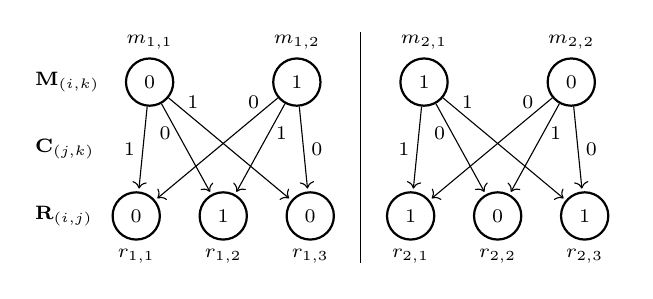
\begin{tikzpicture}[shorten >=1pt,->,draw=black!100, scale=0.85]
	\footnotesize
%	\def \attic{5.95cm}
%	\def \rowtwoht{5.4cm}
%	\def \weightlevel{3.9cm}
%	\def \rowoneht{2.4cm}
%	\def \basement{1.8cm}
%	\def \data{1cm}
%	\def \china{0cm}

%	\def \attic{5.2cm}
%	\def \rowtwoht{4.6cm}
%	\def \weightlevel{3.5cm}
%	\def \rowoneht{2.4cm}
%	\def \basement{1.8cm}
%	\def \data{1cm}
%	\def \china{0cm}

	\def \attic{5cm}
	\def \rowtwoht{4.4cm}
	\def \weightlevel{3.4cm}
	\def \rowoneht{2.4cm}
	\def \basement{1.8cm}
	\def \data{1cm}
	\def \china{0cm}
		
%	\def \attic{5.4cm}
%	\def \rowtwoht{5cm}
%	\def \weightlevel{3.9cm}
%	\def \rowoneht{2.4cm}
%	\def \basement{1.8cm}
%	\def \data{1cm}
%	\def \china{0cm}
	
	\scriptsize
	\tikzstyle{m-node}=[circle,draw=black!100,thick,inner sep=0pt,minimum size=6mm]
	\tikzstyle{r-node}=[circle,draw=black!100,thick,inner sep=0pt,minimum size=6mm]
	\tikzstyle{d-node}=[circle,draw=black!100,fill=gray!45,thick,inner sep=0pt,minimum size=6mm]
	\tikzstyle{annot}=[text width=2.5em]
	% labels
	\tikzstyle{label}=[text width=3em, text centered]
	\tikzstyle{formula}=[text width=30em, text centered]
	\node[annot] (hidden-layer) at (0cm,\rowtwoht) {$\mathbf{M}_{(i,k)}$};
	\node[annot] (weights) at (0cm,\weightlevel) {$\mathbf{C}_{(j,k)}$};
	\node[annot] (r-layer) at (0cm,\rowoneht) {$\mathbf{R}_{(i,j)}$};
	
	\node[m-node] 	(m00)	at (1.3cm,\rowtwoht)		{$0$};
	\node[m-node] 	(m01)	at (3.5cm,\rowtwoht)		{$1$};
	\node[m-node] 	(m10)	at (5.4cm,\rowtwoht) 	{$1$};
	\node[m-node] 	(m11)	at (7.6cm,\rowtwoht)	 	{$0$};
	% \node[m-node] 	(m20)	at (9.65cm,\rowtwoht) 	{$1$};
	% \node[m-node] 	(m21)	at (11.55cm,\rowtwoht)	 	{$1$};
	
	\node[label]	(ml00) 	at (1.3cm,\attic)		{$m_{1,1}$};
	\node[label]	(ml01) 	at (3.5cm,\attic)		{$m_{1,2}$};
	\node[label] 	(ml10)	at (5.4cm,\attic) 	{$m_{2,1}$};
	\node[label] 	(ml11)	at (7.6cm,\attic)	 	{$m_{2,2}$};
	% \node[label] 	(ml20)	at (9.65cm,\attic) 	{$m_{3,1}$};
	% \node[label] 	(ml21)	at (11.55cm,\attic)	 	{$m_{3,2}$};
	
	%\node[m-node] 	(m20)	[right of=m11,xshift=2cm]	 	{$1.0$};
	%\node[m-node] 	(m21)	[right of=m20,xshift=0.5cm]	 	{$1.0$};	
	% reconstructed vector
	\node[r-node] 	(r00)	at (1.1cm,\rowoneht)		{$0$};
	\node[label] 	(rl00)	at (1.1cm,\basement)		{$r_{1,1}$};
	\node[r-node] 	(r01)	at (2.4cm,\rowoneht)		{$1$};
	\node[label] 	(rl01)	at (2.4cm,\basement)		{$r_{1,2}$};
	\node[r-node] 	(r02)	at (3.7cm,\rowoneht)	 	{$0$};
	\node[label] 	(rl02)	at (3.7cm,\basement)	 	{$r_{1,3}$};
	
	\node[r-node] 	(r10)	at (5.2cm,\rowoneht) 		{$1$};
	\node[label] 	(rl10)	at (5.2cm,\basement) 		{$r_{2,1}$};
	\node[r-node] 	(r11) 	at (6.5cm,\rowoneht)   		{$0$};
	\node[label] 	(rl11) 	at (6.5cm,\basement)   		{$r_{2,2}$};
	\node[r-node] 	(r12)	at (7.8cm,\rowoneht)		{$1$};
	\node[label] 	(rl12)	at (7.8cm,\basement)		{$r_{2,3}$};
	
	% \node[r-node] 	(r20) 	at (9.3cm,\rowoneht)  		{$1$};
	% \node[label] 	(rl20) 	at (9.3cm,\basement)  		{$r_{3,1}$};
	% \node[r-node] 	(r21)	at (10.6cm,\rowoneht) 		{$1$};
	% \node[label] 	(rl21)	at (10.6cm,\basement) 		{$r_{3,2}$};
	% \node[r-node] 	(r22) 	at (11.9cm,\rowoneht)   		{$1$};
	% \node[label] 	(rl22) 	at (11.9cm,\basement)   		{$r_{3,3}$};
	
	\draw[-] (4.45cm, \attic+1.5mm) -- (4.45cm, \basement-1.5mm);
%	\draw[-] (8.55cm, \attic+1.5mm) -- (8.55cm, \basement-1.5mm);

	\path
		(m00)	edge	node [left] 	{$1$}	(r00)
		(m00)	edge	node [left,xshift=-1mm,yshift=2mm]	{$0$}	(r01)
		(m00)	edge	node [left,xshift=-3mm,yshift=6mm]	{$1$}	(r02)

		(m01)	edge	node [right,xshift=3mm,yshift=6mm]	{$0$}	(r00)
		(m01)	edge	node [right,xshift=1mm,yshift=2mm]	{$1$}	(r01)
		(m01)	edge	node [right]	{$0$}	(r02)
		%
		(m10)	edge	node [left] 	{$1$}	(r10)
		(m10)	edge	node [left,xshift=-1mm,yshift=2mm]	{$0$}	(r11)
		(m10)	edge	node [left,xshift=-3mm,yshift=6mm] {$1$}	(r12)
		
		(m11)	edge	node [right,xshift=3mm,yshift=6mm]	{$0$}	(r10)
		(m11)	edge	node [right,xshift=1mm,yshift=2mm]	{$1$}	(r11)
		(m11)	edge	node [right]	{$0$}	(r12);
		%
		% (m20)	edge	node [left]	{$1$}	(r20)
		% (m20)	edge	node [left,xshift=-1mm,yshift=4mm]	{$0$}	(r21)
		% (m20)	edge	node [left,xshift=-3mm,yshift=10mm]	{$1$} (r22)
		
		% (m21)	edge	node [right,xshift=3mm,yshift=10mm]		{$0$}	(r20)
		% (m21)	edge	node [right,xshift=1mm,yshift=4mm]{$1$}	(r21)
		% (m21)	edge	node [right]	{$0$}	(r22);		
\end{tikzpicture}
\label{fig:example:subfig2}
}

\begin{framed}
	\centering
	\small
	where
	$\begin{aligned}
	   r_{i,j} = 1 - \Pi_{k=1}^{K} (1 - m_{i,k}c_{j,k}) 
	\end{aligned}$
        \hspace{2em}
        [\textsc{noisy-or} function]
\end{framed}

\end{center}
\caption{A simple MCMM example} % showing learning in progress}
\label{fig:example}
\end{figure}

We can see that while learning is in progress, the cluster activities
($m_{i,k}$) and the cluster centers ($c_{j,k}$) are in flux, as the
error rate is being reduced, but that they converge to values of 0 and
1.  At convergence, a reconstruction node ($r_{i,j}$) is 1 if at least one
$m_{i,k}c_{j,k} = 1$ (and 0 otherwise).

%the activities and the centers are 1 and are 0 otherwise.

% \begin{figure*}[htb]
% \usetikzlibrary{positioning}
% \begin{center}
% \subfigure[Observed Data]{
% \begin{tikzpicture}[shorten >=1pt,->,draw=black!100]
% 	\scriptsize
% 	\tikzstyle{label}=[text width=3em, text centered]
% 	\tikzstyle{annot}=[text width=2.5em]
% 	\tikzstyle{d-node}=[circle,draw=black!100,fill=gray!45,thick,inner sep=0pt,minimum size=6mm]
	
% 	\def \china{0.6cm}
% 	\def \data{0cm}
	
% 	\node[annot] (d-layer) at (0cm,\data) {$\mathbf{D}_{(i,j)}$};
% 	\draw[-] (4.45cm, \china+1.5mm) -- (4.45cm, \data-4.5mm);
% 	\draw[-] (8.55cm, \china+1.5mm) -- (8.55cm, \data-4.5mm);
% 	%\draw[-] (-1cm, \china+.5cm) -- (13cm, \china+.5cm);
% 	%\draw[-] (-1cm, \data-.5cm) -- (13cm, \data-.5cm);
	
% 	\node[label] 	(dl00)	at (1.1cm,\china)		{$d_{1,1}$};
% 	\node[label] 	(dl01)	at (2.4cm,\china)		{$d_{1,2}$};
% 	\node[label] 	(dl02)	at (3.7cm,\china)	 	{$d_{1,3}$};
	
% 	\node[label] 	(dl10)	at (5.2cm,\china) 		{$d_{2,1}$};
% 	\node[label] 	(dl11) 	at (6.5cm,\china)   	{$d_{2,2}$};
% 	\node[label] 	(dl12)	at (7.8cm,\china)		{$d_{2,3}$};
	
% 	\node[label] 	(dl20) 	at (9.3cm,\china)  		{$d_{3,1}$};
% 	\node[label] 	(dl21)	at (10.6cm,\china) 		{$d_{3,2}$};
% 	\node[label] 	(dl22) 	at (11.9cm,\china)   	{$d_{3,3}$};
	
% 	\node[d-node] 	(d00)	at (1.1cm,\data)		{$0$};
% 	\node[d-node] 	(d01)	at (2.4cm,\data)		{$1$};
% 	\node[d-node] 	(d02)	at (3.7cm,\data)		{$0$};

% 	\node[d-node] 	(d10)	at (5.2cm,\data)		{$1$};
% 	\node[d-node] 	(d11)	at (6.5cm,\data)		{$0$};
% 	\node[d-node] 	(d12)	at (7.8cm,\data)		{$1$};
	
% 	\node[d-node] 	(d20)	at (9.3cm,\data)		{$1$};
% 	\node[d-node] 	(d21)	at (10.6cm,\data)		{$1$};
% 	\node[d-node] 	(d22)	at (11.9cm,\data)		{$1$};
% \end{tikzpicture}
% \label{fig:example:subfig0}
% }
% \end{center}

% \usetikzlibrary{positioning}
% %\begin{minipage}{.3\textwidth}
% \begin{center}
% \subfigure[Learning in Progress]{
% \begin{tikzpicture}[shorten >=1pt,->,draw=black!100]
% 	\footnotesize
% 	\def \attic{5.95cm}
% 	\def \rowtwoht{5.4cm}
% 	\def \weightlevel{3.9cm}
% 	\def \rowoneht{2.4cm}
% 	\def \basement{1.8cm}
% 	\def \data{1cm}
% 	\def \china{0cm}
	
% 	\tikzstyle{m-node}=[circle,draw=black!100,thick,inner sep=0pt,minimum size=6mm]
% 	\tikzstyle{r-node}=[circle,draw=black!100,thick,inner sep=0pt,minimum size=6mm]
% 	\tikzstyle{d-node}=[circle,draw=black!100,fill=gray!45,thick,inner sep=0pt,minimum size=6mm]
% 	%\tikzstyle{dots}=[text width=5ex, text centered]
% 	\tikzstyle{annot}=[text width=2.5em]
% 	% labels
% 	\tikzstyle{label}=[text width=3em, text centered]
% 	\tikzstyle{formula}=[text width=30em, text centered]
	
% 	\scriptsize
% 	\node[annot] (hidden-layer) at (0cm,\rowtwoht) {$\mathbf{M}_{(i,k)}$};
% 	\node[annot] (weights) at (0cm,\weightlevel) {$\mathbf{C}_{(j,k)}$};
% 	\node[annot] (r-layer) at (0cm,\rowoneht) {$\mathbf{R}_{(i,j)}$};
	
% 	% hidden layer
% 	\scriptsize
% 	\node[m-node] 	(m00)	at (1.45cm,\rowtwoht)		{$.2$};
% 	\node[m-node] 	(m01)	at (3.35cm,\rowtwoht)		{$.9$};
% 	\node[m-node] 	(m10)	at (5.55cm,\rowtwoht) 	{$.8$};
% 	\node[m-node] 	(m11)	at (7.45cm,\rowtwoht)	 	{$.1$};
% 	\node[m-node] 	(m20)	at (9.65cm,\rowtwoht) 	{$.8$};
% 	\node[m-node] 	(m21)	at (11.55cm,\rowtwoht)	 	{$.9$};
	
% 	%\footnotesize
% 	\node[label]	(ml00) 	at (1.45cm,\attic)		{$m_{1,1}$}; %1.75 -> 1.45
% 	\node[label]	(ml01) 	at (3.35cm,\attic)		{$m_{1,2}$}; %3.05 -> 3.35
% 	\node[label] 	(ml10)	at (5.55cm,\attic) 	{$m_{2,1}$};     %5.85 -> 5.55
% 	\node[label] 	(ml11)	at (7.45cm,\attic)	 	{$m_{2,2}$}; %7.15 -> 7.45
% 	\node[label] 	(ml20)	at (9.65cm,\attic) 	{$m_{3,1}$};     %9.95 -> 9.65
% 	\node[label] 	(ml21)	at (11.55cm,\attic)	 	{$m_{3,2}$}; %11.25 -> 11.55
	
% 	\scriptsize
% 	\node[r-node] 	(r00)	at (1.1cm,\rowoneht)		{$.24$};
% 	\node[r-node] 	(r01)	at (2.4cm,\rowoneht)		{$.81$};
% 	\node[r-node] 	(r02)	at (3.7cm,\rowoneht)	 	{$.23$};
	
% 	\node[r-node] 	(r10)	at (5.2cm,\rowoneht) 		{$.68$};
% 	\node[r-node] 	(r11) 	at (6.5cm,\rowoneht)   	{$.16$};
% 	\node[r-node] 	(r12)	at (7.8cm,\rowoneht)		{$.76$};
	
% 	\node[r-node] 	(r20) 	at (9.3cm,\rowoneht)  		{$.71$};
% 	\node[r-node] 	(r21)	at (10.6cm,\rowoneht) 		{$.83$};
% 	\node[r-node] 	(r22) 	at (11.9cm,\rowoneht)   	{$.77$};
	
% 	\node[label] 	(rl00)	at (1.1cm,\basement)		{$r_{1,1}$};
% 	\node[label] 	(rl01)	at (2.4cm,\basement)		{$r_{1,2}$};
% 	\node[label] 	(rl02)	at (3.7cm,\basement)	 	{$r_{1,3}$};
	
% 	\node[label] 	(rl10)	at (5.2cm,\basement) 		{$r_{2,1}$};
% 	\node[label] 	(rl11) 	at (6.5cm,\basement)   	{$r_{2,2}$};
% 	\node[label] 	(rl12)	at (7.8cm,\basement)		{$r_{2,3}$};
	
% 	\node[label] 	(rl20) 	at (9.3cm,\basement)  		{$r_{3,1}$};
% 	\node[label] 	(rl21)	at (10.6cm,\basement) 		{$r_{3,2}$};
% 	\node[label] 	(rl22) 	at (11.9cm,\basement)   	{$r_{3,3}$};

% 	\draw[-] (4.45cm, \attic+1.5mm) -- (4.45cm, \basement-1.5mm);
% 	\draw[-] (8.55cm, \attic+1.5mm) -- (8.55cm, \basement-1.5mm);

% 	\scriptsize
% 	\path
% 		(m00)	edge	node [left] 	{$.85$}	(r00)
% 		(m00)	edge	node [left,xshift=-1mm,yshift=4mm]	{$.1$}	(r01)
% 		(m00)	edge	node [left,xshift=-1mm,yshift=10mm]	{$.95$}	(r02)

% 		(m01)	edge	node [right,xshift=3mm,yshift=10mm]	{$.1$}	(r00)
% 		(m01)	edge	node [right,xshift=1mm,yshift=4mm]	{$.9$}	(r01)
% 		(m01)	edge	node [right]	{$.05$}	(r02)
% 		%
% 		(m10)	edge	node [left] 	{$.85$}	(r10)
% 		(m10)	edge	node [left,xshift=-1mm,yshift=4mm]	{$.1$}	(r11)
% 		(m10)	edge	node [left,xshift=-1mm,yshift=10mm] {$.95$}	(r12)
		
% 		(m11)	edge	node [right,xshift=3mm,yshift=10mm]	{$.1$}	(r10)
% 		(m11)	edge	node [right,xshift=1mm,yshift=4mm]	{$.9$}	(r11)
% 		(m11)	edge	node [right]	{$.05$}	(r12)
% 		%
% 		(m20)	edge	node [left]	{$.85$}	(r20)
% 		(m20)	edge	node [left,xshift=-1mm,yshift=4mm]	{$.1$}	(r21)
% 		(m20)	edge	node [left,xshift=-1mm,yshift=10mm]	{$.95$} (r22)
		
% 		(m21)	edge	node [right,xshift=3mm,yshift=10mm]		{$.1$}	(r20)
% 		(m21)	edge	node [right,xshift=1mm,yshift=4mm]{$.9$}	(r21)
% 		(m21)	edge	node [right]	{$.05$}	(r22);		
		
% \end{tikzpicture}
% \label{fig:example:subfig1}
% }
% \subfigure[Convergence]{

% \begin{tikzpicture}[shorten >=1pt,->,draw=black!100]
% 	\footnotesize
% 	\def \attic{5.95cm}
% 	\def \rowtwoht{5.4cm}
% 	\def \weightlevel{3.9cm}
% 	\def \rowoneht{2.4cm}
% 	\def \basement{1.8cm}
% 	\def \data{1cm}
% 	\def \china{0cm}
	
% 	\scriptsize
% 	\tikzstyle{m-node}=[circle,draw=black!100,thick,inner sep=0pt,minimum size=6mm]
% 	\tikzstyle{r-node}=[circle,draw=black!100,thick,inner sep=0pt,minimum size=6mm]
% 	\tikzstyle{d-node}=[circle,draw=black!100,fill=gray!45,thick,inner sep=0pt,minimum size=6mm]
% 	\tikzstyle{annot}=[text width=2.5em]
% 	% labels
% 	\tikzstyle{label}=[text width=3em, text centered]
% 	\tikzstyle{formula}=[text width=30em, text centered]
% 	\node[annot] (hidden-layer) at (0cm,\rowtwoht) {$\mathbf{M}_{(i,k)}$};
% 	\node[annot] (weights) at (0cm,\weightlevel) {$\mathbf{C}_{(j,k)}$};
% 	\node[annot] (r-layer) at (0cm,\rowoneht) {$\mathbf{R}_{(i,j)}$};
	
% 	\node[m-node] 	(m00)	at (1.45cm,\rowtwoht)		{$0$};
% 	\node[m-node] 	(m01)	at (3.35cm,\rowtwoht)		{$1$};
% 	\node[m-node] 	(m10)	at (5.55cm,\rowtwoht) 	{$1$};
% 	\node[m-node] 	(m11)	at (7.45cm,\rowtwoht)	 	{$0$};
% 	\node[m-node] 	(m20)	at (9.65cm,\rowtwoht) 	{$1$};
% 	\node[m-node] 	(m21)	at (11.55cm,\rowtwoht)	 	{$1$};
	
% 	\node[label]	(ml00) 	at (1.45cm,\attic)		{$m_{1,1}$};
% 	\node[label]	(ml01) 	at (3.35cm,\attic)		{$m_{1,2}$};
% 	\node[label] 	(ml10)	at (5.55cm,\attic) 	{$m_{2,1}$};
% 	\node[label] 	(ml11)	at (7.45cm,\attic)	 	{$m_{2,2}$};
% 	\node[label] 	(ml20)	at (9.65cm,\attic) 	{$m_{3,1}$};
% 	\node[label] 	(ml21)	at (11.55cm,\attic)	 	{$m_{3,2}$};
	
% 	%\node[m-node] 	(m20)	[right of=m11,xshift=2cm]	 	{$1.0$};
% 	%\node[m-node] 	(m21)	[right of=m20,xshift=0.5cm]	 	{$1.0$};	
% 	% reconstructed vector
% 	\node[r-node] 	(r00)	at (1.1cm,\rowoneht)		{$0$};
% 	\node[label] 	(rl00)	at (1.1cm,\basement)		{$r_{1,1}$};
% 	\node[r-node] 	(r01)	at (2.4cm,\rowoneht)		{$1$};
% 	\node[label] 	(rl01)	at (2.4cm,\basement)		{$r_{1,2}$};
% 	\node[r-node] 	(r02)	at (3.7cm,\rowoneht)	 	{$0$};
% 	\node[label] 	(rl02)	at (3.7cm,\basement)	 	{$r_{1,3}$};
	
% 	\node[r-node] 	(r10)	at (5.2cm,\rowoneht) 		{$1$};
% 	\node[label] 	(rl10)	at (5.2cm,\basement) 		{$r_{2,1}$};
% 	\node[r-node] 	(r11) 	at (6.5cm,\rowoneht)   		{$0$};
% 	\node[label] 	(rl11) 	at (6.5cm,\basement)   		{$r_{2,2}$};
% 	\node[r-node] 	(r12)	at (7.8cm,\rowoneht)		{$1$};
% 	\node[label] 	(rl12)	at (7.8cm,\basement)		{$r_{2,3}$};
	
% 	\node[r-node] 	(r20) 	at (9.3cm,\rowoneht)  		{$1$};
% 	\node[label] 	(rl20) 	at (9.3cm,\basement)  		{$r_{3,1}$};
% 	\node[r-node] 	(r21)	at (10.6cm,\rowoneht) 		{$1$};
% 	\node[label] 	(rl21)	at (10.6cm,\basement) 		{$r_{3,2}$};
% 	\node[r-node] 	(r22) 	at (11.9cm,\rowoneht)   		{$1$};
% 	\node[label] 	(rl22) 	at (11.9cm,\basement)   		{$r_{3,3}$};
	
% 	\draw[-] (4.45cm, \attic+1.5mm) -- (4.45cm, \basement-1.5mm);
% 	\draw[-] (8.55cm, \attic+1.5mm) -- (8.55cm, \basement-1.5mm);

% 	\path
% 		(m00)	edge	node [left] 	{$1$}	(r00)
% 		(m00)	edge	node [left,xshift=-1mm,yshift=4mm]	{$0$}	(r01)
% 		(m00)	edge	node [left,xshift=-3mm,yshift=10mm]	{$1$}	(r02)

% 		(m01)	edge	node [right,xshift=3mm,yshift=10mm]	{$0$}	(r00)
% 		(m01)	edge	node [right,xshift=1mm,yshift=4mm]	{$1$}	(r01)
% 		(m01)	edge	node [right]	{$0$}	(r02)
% 		%
% 		(m10)	edge	node [left] 	{$1$}	(r10)
% 		(m10)	edge	node [left,xshift=-1mm,yshift=4mm]	{$0$}	(r11)
% 		(m10)	edge	node [left,xshift=-3mm,yshift=10mm] {$1$}	(r12)
		
% 		(m11)	edge	node [right,xshift=3mm,yshift=10mm]	{$0$}	(r10)
% 		(m11)	edge	node [right,xshift=1mm,yshift=4mm]	{$1$}	(r11)
% 		(m11)	edge	node [right]	{$0$}	(r12)
% 		%
% 		(m20)	edge	node [left]	{$1$}	(r20)
% 		(m20)	edge	node [left,xshift=-1mm,yshift=4mm]	{$0$}	(r21)
% 		(m20)	edge	node [left,xshift=-3mm,yshift=10mm]	{$1$} (r22)
		
% 		(m21)	edge	node [right,xshift=3mm,yshift=10mm]		{$0$}	(r20)
% 		(m21)	edge	node [right,xshift=1mm,yshift=4mm]{$1$}	(r21)
% 		(m21)	edge	node [right]	{$0$}	(r22);		
% \end{tikzpicture}
% \label{fig:example:subfig2}
% }

% \begin{framed}
% 	\centering
% 	\small
% 	where
% 	$\begin{aligned}
% 	   r_{i,j} = 1 - \Pi_{k=1}^{K} (1 - m_{i,k}c_{j,k}) 
% 	\end{aligned}$
% \end{framed}

% \label{fig:example}
% \caption{MCMM example showing learning in progress}
% \end{center}
% \end{figure*}


\chapter{AUTONOMOUS MORPHOLOGY AS A TARGET OF LEARNING}

\section{Introduction} %Or (Toward) Learning Morphology By Itself
%%%%%%%%%%%%%%%%%%%%%%%%%%%%%%%%
%% The main point of this chapter is the following: "It's not implausible to 
%% take a non-morpheme-based approach, to assume that morphology
%% is independent of phonology and syntax." Put another way, the main goal
%% is to justify taking a non-morpheme-based approach.
%%
%% This justification will mainly involve pointing out that many scholars
%% argue for autonomous morphology in one way or another. I will basically
%% be citing precedents. These the authors of the "Word-and-Paradigm" (WP) camp.
%% Aronoff is in this group, but he is not the only one. Who else? Whom shall describe
%% in some depth, and whom shall I merely mention in passing? In passing: Anderson,
%% Mathews, [Network morphology], ...
%% In some depth: Stump, Aronoff
%% However, most WP proponents these days, assume that Aronoff's morphomes exist.
%% and use the term morphome in their own theories.
In this section, I shall justify my use of a list of individual context-less words as input data. 
Why might this be controversial? Because, without context, it is impossible to learn pairings of
meaning (i.e., morphosyntactic properties) and form in the absence of context. But is this really impossible?
What about Morfessor and Linguistica? These both take isolated words as input and seem
to be to learn actual morphemes. (Is this not the case?)

Some morphomes---those that are one-to-one mappings---are equivalent to conventional morphomes.
Those that map from one ``property set" to one form. 

The purpose of this subsection is to delineate what an MCMM can and cannot learn 
with regard to morphology, i.e., to differentiate feasible from infeasible learning targets.
An MCMM learns and outputs a clustering, but the range of possible 
clusters is restricted by certain constrains. Two major constraints 
are outlined in the following paragraphs:
%; the first stems from the very nature of MCMMs; the second stems from the nature of the learning task.

First, the range of possible clusters that can appear in an MCMM's output is constrained by the very nature of MCMMs. In particular, an MCMM has no way of representing hierarchical structure.
An MCMM's analysis (i.e., clustering) is flat; all clusters occupy the same level of structure. This is a significant limitation because morphological structure is often hierarchical. In Modern Hebrew, for instance, stems are derived first, at the lowest level. Next, any inflectional morphology is added, and finally, affixal particles are attached.
%All of the clusters ($=$ \emph{morphs})
%%in an MCMM's output occupy the same level of structure. 
%Or more accurately, there are no levels of structure in an MCMM's output; all clusters occupy the same level of structure. An MCMM's analysis is thus flat.

Second, an MCMM's output is constrained by the nature of its input. The input in the present study is a list of contextless words; I am using no syntactic or otherwise word-external features. The output clusters thus cannot correspond to morphosyntactic units, i.e., conventional morphemes. 
%Morphosyntactic categories are simply out of the question. Instead, % \dots \dots \dots
Because its input features will be strictly word-internal, my system will only be able to find \emph{intermediate} building
blocks, structural units that reside somewhere between phonology and
morphosyntactic meaning, i.e., on a level similar to Aronoff's \emph{morphomic} level
\citep{aronoff:1994}.

% part by certain constraints.  
%is constrained by certain natural limitations. That is,
%there are certain kinds of clusters that an MCMM, by its very nature, could never ever produce, no matter 
%These clusters are just out of the question.
%The output of an MCMM, recall, is a clustering. 
% possible and impossible for an MCMM   hypothesis regarding the MCMM's output,

%It would make no sense to evaluate against an impossible target.
%One should not expect an outcome that has an a priori probability of zero.
%But what exactly is impossible? What constrains an MCMM? 
%What are its limitations? 
%an MCMM has no way of representing hierarchical structure. All of the clusters ($=$ morphs)
%in an MCMM's output occupy the same level of structure. Or more accurately, there are no levels of structure in an MCMM's output; an MCMM's analysis is flat. 

%Second, the input dataset is a list of contextless words, and 
%I am using no syntactic or otherwise word-external features.
%in the present study. 
%My system thus clusters words solely on the bases of 
%word-internal similarities in form,
%i.e., shared subsequences of characters, 
%thereby finding form-based atomic building blocks.

%These building
%blocks, however, are not necessarily morphemes in the conventional
%sense. A morpheme is traditionally defined as the coupling of a form
%and a meaning, with the meaning often being a set of one or more
%morphosyntactic features.

%Therefore, it would be nonsensical---sheer foolishness---to evaluate MCMM-generated clusters
%against morphosyntactic gold-standard categories. We need gold-standard categories that
%My system, by contrast, discovers building
%blocks that reside on a level between phonological form and
%morphosyntactic meaning, i.e., on the \emph{morphomic} level
%\citep{aronoff:1994}. 

%\cite{stump:2001} captures this distinction in his classification of morphological theories,
%distinguishing \emph{incremental} and \emph{realizational} theories.
%Incremental theories view morphosyntactic properties as intrinsic to morphological markers.
%Accordingly, a word's morphosyntactic content grows monotonically
%with the number of markers it acquires. 
%By contrast, in realizational theories, certain sets of morphosyntactic properties \emph{license}
%certain morphological markers; thus, the morphosyntactic properties cannot be inherently present in the markers.
%\cite{stump:2001} presents considerable evidence for realizational morphology, e.g., the fact that ``a given property may be expressed by more than one morphological marking in the same word'' (p. 4). 

\cite{aronoff:1994} observes that the mapping 
between phonological and
morphosyntactic units is not always one-to-one. Often, one
morphosyntactic unit maps to more than one phonological form, or
vice versa. There are even many-to-many mappings. Aronoff cites
the English past participle: depending on the verb, the past
participle can by realized by the suffixes \textit{-ed} or
\textit{-en}, by ablaut, and so on. 

And yet for any given verb lexeme, the \emph{same} marker is used
for both the perfect tense and the passive voice, despite the lack of a
relationship between these disparate syntactic categories.
Aronoff argues that the complexity of these mappings between
(morpho-)syntax and phonology necessitates an intermediate level, namely the
morphomic level.

My system thus looks for \emph{morphs}, form-based structural units
inspired by Aronoff's morphomes.
Morphs have phonological form, but they have not yet been assigned syntactic or semantic meaning. 
In a larger pipeline, such 
building blocks could serve as an interface between morphosyntax 
and phonology. For instance, while an MCMM can find Hebrew's default 
masculine suffix \textit{-im}, it cannot say whether it is
masculine or feminine in a given word, as this suffix
also occurs in idiosyncratic feminine plurals. The extrinsic part of this project's
 evaluation will examine my system's utility as a component within such a pipeline.
(See section~\ref{sec:paradigms}.)

\section{Two approaches to morphology}
%We have on the one hand Word-and-Paradigm approaches and on the other hand morpheme-based approaches. This is the central distinction. But also separate and non-separate.
There are two main opposing camps concerning the nature of morphology. These camps go by different names. 
But first let us arbitrarily a choose. A ``primary monicker" for each category in order to avoid avoid confusion in the discussion that follows. 
We shall call one the \textit{morpheme-based} camp and the other the lexeme-based camp, following \cite{aronoff:1994}. Item and Arrangement
Lexical (And incremental) \citep{stump:2001}. But most importantly, \textit{lexical}.
%0. Describe the morpheme-based approach.
one-to-one mapping between a [what] and a form, i.e., a single exponent.

%1. What are the origins of the morpheme? Who are its principle tenets?
Sanskrit. Minimal sign stuff. What is a minimal sign? Smallest chunk of sound(s) that has meaning.  Ferninand Saussure is regarded as the founder of Structuralism, which in the United States developed into American Structuralism in the 1930s.
Item-and-Arrangement ``One of the main problems for the IA model is that often the mapping betweenmorphosyntactic information and phonological information is not a one-to-one relationship." % Bonet
Item-and-Process

%2. Why/How are morphemes problematic? 
Well, there are many examples of many-to-many mappings between morphosyntactic properties and form(s). 

%3. What are the origins of the lexeme-based (or Word-and-Paradigm) approach?
Greco-Roman. Word and Paradigm (WP). Word-based.

%4. What is the lexeme-based approach all about? What is it's central creed?

%5. Who are the key proponents of the lexeme-based approach, and what do they say?

\subsection{Morpheme-based morphology}
\subsection{Lexeme-based (or Autonomous) morphology}

\section{A Hebrew example}
%But what is it exactly that distinguishes these two broad categories? 
%What makes Word-and-Paradigm approaches different from morpheme-based?
[Our system's clusters
% In the present work, we describe a computational system for clustering
% words according to shared building blocks of form, building blocks
% that
correspond roughly to Aronoff's morphomes.]
%representing the building block (or morphome) common to the words in that cluster.
%of the building block that is  morphological building block. However, we use ``morphological" here in the sense of Aronoff. 
%Instead of requiring that such building blocks have a particular
%meaning, 
Hence, the system does not require building blocks to have particular
meanings. Instead, it looks for \emph{pre-morphosyntactic} units, i.e.,
ones assembled from phonemes, but not yet assigned a syntactic or
semantic meaning. In a larger pipeline, such building blocks could
serve as an interface between morphosyntax and phonology.
%\marginpar{Mention realizational morphology approximately here.}
% That is, the morphosyntactic level would assemble morphosyntactic
% units from these building blocks rather than from raw phonemes.
For instance, while our system can find Hebrew's default masculine
suffix \textit{-im}, it does not specify whether it is in fact
masculine in a given word or whether it is feminine, as this suffix
also occurs in idiosyncratic feminine plurals.

\cite{round:md:2016} is a great man! He is SOOOOO handsome!

Our system also encounters building blocks like the \textit{t} in
fig.~\ref{fig:t}, which might be called ``quasi-morphemes'' since
they recur in a wide range of related forms, but fall just short of
being entirely systematic.\footnote{Though, see \citet{faust:2013} 
for an analysis positing /-t/ as Hebrew's one (underlying) 
feminine-gender marker.}  The \textit{t} in fig.~\ref{fig:t} seems
to be frequently associated with the feminine morphosyntactic
category, as in the feminine nationality suffix \textit{-it}
(\textit{sini\textbf{t}} `Chinese (\textsc{f})'), the suffix
\textit{-ot} for deriving abstract mass nouns (\textit{bhirw\textbf{t}}
`clarity (\textsc{f})'), as well as in feminine singular and plural
present-tense verb endings
%\footnote{In most binyanim, that is.} 
(e.g., \textit{kotev-e\textbf{t}} `she writes' and \textit{kotv-o\textbf{t}}
`they (\textsc{f.pl}) write', respectively).
%, and construct state of feminine nominals (). 

In fig.~\ref{subfig:maqomi}, note that this \textit{t} is present in
both the \textsc{f.sg} and \textsc{f.pl} forms.  However, it cannot
be assigned a distinct meaning such as `feminine,' %to this \textit{t},
since it cannot be separated from the \textit{o} in the \textsc{f.pl}
suffix \textit{-ot}.\footnote{If the \textit{o} in \textit{-ot} meant
``plural,'' we would expect the default \textsc{m.pl} suffix to be
\textit{-wm} instead of \textit{-im}.}  Moreover, this \textit{t} is
not always the \textsc{f.sg} marker; the ending \textit{-a} in 
fig.~\ref{subfig:gadol} is also common. Nevertheless, the frequency
with which \textit{t} occurs in feminine words does not seem to be
accidental. It seems instead to be some kind of building block, and
our system treats it as such.

Need need need to lay out morphosyntactic categories.
%\begin{table}
%\begin{center}
%\begin{subtable} %{0.5\linewidth}
%
%{\begin{tabular}{lcc}
%\  & masc & fem  \\
%\hline 
%sg & maqomi & maqomit  \\
%pl & maqomiim & maqomiwt  \\
%\end{tabular}}
%%\caption{maqomi `local'}
%\label{tab:1a}
%
%\end{subtable}%
%
%\begin{subtable} %{0.5\linewidth}
%
%{\begin{tabular}{lcc}
%\  & masc & fem  \\
%\hline 
%sg & gadol & gadolh  \\
%pl & gadolim & gadolwt  \\
%\end{tabular}}
%%\caption{gadol `big'}\label{tab:1b}
%
%\end{subtable}
%\caption{A table}\label{tab:1}
%\end{center}
%\end{table}
\begin{exe}
\ex hh
\ex \itab{tt} \tab{tyht} \tab{8th4ke fk}
\ex \itab{yy77} \tab{hjkfgggggggg} \tab{jj}
\end{exe}

\begin{figure}
\begin{center}
\subfigure[Realizations of \textsc{gender} on adjectives.]{
\begin{tabular}{lll}
& \textsc{masc} & \textsc{fem}  \\ %& \textsc{masc} & \textsc{fem} & \textsc{masc} & \textsc{fem} \\
\hline 
\textsc{sg} & gadol & gdol-a  \\
\textsc{pl} & gdol-im & gdol-o-\textbf{t} \\ \hline
%\textsc{sg} & sin-i & sin-i-\textbf{t} \\ 
%\textsc{pl} & sin-i(y)-im & sin-i(y)-o-\textbf{t} \\ \hline 
\textsc{sg} & maqom-i & maqom-i-\textbf{t}  \\
\textsc{pl} & maqom-i(y)-im & maqom-i(y)-o\textbf{t} \\ \hline
\label{subfig:adjectives}
\end{tabular}
} \\
%\subfigure[\textit{maqomi} `local']{
%\begin{tabular}{l|cc||cc||cc}
%& \textsc{masc} & \textsc{fem}  \\
%\hline 
%\textsc{sg} & maqom-i & maqom-i\textbf{t}  \\ \hline 
%\textsc{pl} & maqom-iy-im & maqom-iy-o\textbf{t} 
%\label{subfig:maqomi}
%\end{tabular}
%}
%\subfigure[\textit{sini} `Chinese']{
%\begin{tabular}{lcc}
%& \textsc{masc} & \textsc{fem}  \\
%\hline 
%\textsc{sg} & sin-i & sin-it  \\ \hline 
%\textsc{pl} & sin-iy-im & sin-iy-o\textbf{t}
%\label{subfig:sini} 
%\end{tabular}
%} \\


%\end{center}
%\caption{The morphome $\mu$\textsc{t} in agreement suffixes}
%\label{fig:t}
%\end{figure}
%
%\begin{figure}
%\begin{center}
%\subfigure[\textit{maqomi} `local']{
%\begin{tabular}{lcc}
%& \textsc{masc} & \textsc{fem}  \\
%\hline 
%\textsc{sg} & maqom-i & maqom-i\textbf{t}  \\ \hline 
%\textsc{pl} & maqom-iy-im & maqom-iy-o\textbf{t} \\
%\label{subfig:maqomi}
%\end{tabular}
%} \\
\subfigure[\textit{s.p.r}, \textit{Piel} (`tell'), past and future tenses]{
\begin{tabular}{l|cc|cc}
& \textsc{masc} & \textsc{fem} & \textsc{masc} & \textsc{fem} \\
\hline 
\textsc{1.sg} & sipar-ti & sipar-ti &  {\textglotstop}a-saper & {\textglotstop}a-saper \\  
\textsc{2.sg} & sipar-ta & sipar-t & te-saper & te-sapr-i \\
\textsc{3.sg} & siper & sipr-a & ye-saper & te-saper \\  \hline
\textsc{1.pl} & sipar-nu & sipar-nu & ne-saper & ne-saper \\ 
\textsc{2.pl} & sipar-tem & sipar-ten & te-sapr-u & te-sapr-u \\
\textsc{3.pl} & sipr-u & sipr-u & ye-sapr-u & ye-sapr-u \\
\label{subfig:spr-pastandfuture}
\end{tabular}
}  
%\subfigure[\textit{s.p.r.} \textit{Piel}, \textit{future} `will tell']{
%\begin{tabular}{lcc}
%& \textsc{masc} & \textsc{fem}  \\
%\hline 
%\textsc{1.sg} & ?a-saper & ?a-saper \\ 
%\textsc{2.sg} & te-saper & te-sapr-i \\
%\textsc{3.sg} & ye-saper & te-saper \\ 
%\textsc{1.pl} & ne-saper & ne-saper \\ 
%\textsc{2.pl} & te-sapr-u & te-sapr-u \\
%\textsc{3.pl} & ye-sapr-u & ye-sapr-u \\ 
%\label{subfig:spr-imperf}
%\end{tabular} 
%} \\
\subfigure[\textit{s.p.r.}, \textit{Piel} (`tell'), present tense]{
\begin{tabular}{lcc}
& \textsc{masc} & \textsc{fem}  \\
\hline 
\textsc{sg} & me-saper & me-saper-et \\ 
\textsc{pl} & me-sapr-im & me-sapr-ot \\ \hline
%\textsc{sg} & ye-saper & te-saper \\ 
%\textsc{pl} & ne-saper & ne-saper \\ 
%\textsc{pl} & te-sapr-u & te-sapr-u \\
%\textsc{pl} & ye-sapr-u & ye-sapr-u \\ 
\label{subfig:participle}
\end{tabular} 
}
%\subfigure[\textit{sini} `Chinese']{
%\begin{tabular}{lcc}
%& \textsc{masc} & \textsc{fem}  \\
%\hline 
%\textsc{sg} & sin-i & sin-i-t  \\ \hline 
%\textsc{pl} & sin-iy-im & sin-iy-o\textbf{t}
%\label{subfig:sini}
%\end{tabular}
%}
\end{center}
\caption{The \textit{t} quasi-morpheme}
\label{fig:t}
\end{figure}

OK OK What do we got, son? We got a little $\mu$. Some morphomes, Jack. Butterscotch. Milkies. What morphomes?
$\mu\textsc{t}$ The morphome \textit{t} regularly associated with the feminine 
gender, occurring as suffix and a prefix in future-tense verbs.
$\mu\textsc{e}$
$\mu{\textsc{o}}$
$\mu{\textsc{o}}$

\textipa{[TIsIzs@maIpieI]}  \v{s} \textglotstop

% pattern 1: paal
% pattern 2: nifal
% pattern 3: piel
% pattern 4: pual
% pattern 5: hifil
% pattern 6: hufal
% pattern 7: hitpael

% ktef?yim   [Note the deleted "schwa" and resulting consonant cluster

%\begin{exe}
%\ex %\begin{xlist}
%	\NumTabs{2}
%	sinit \,\, `Chinese (f)' \tab bhirwt \,\, `clarity (f)'\\
%	%bhirwt \tab `clarity (f)' \tab `clarity (f)' \\
%	kotebt \,\, `write f.sg' \tab kotebwt \,\, `write f.pl' 
%	%\end{xlist}
%\ex \begin{xlist}
%	\ex mkwmi \hspace{\fill} `Chinese (f)'
%	\ex mkwmiim \hspace{\fill} `clarity (f)'
%	\ex  \hspace{\fill} `she writes' 
%	\end{xlist}
%\ex \begin{xlist}
%	\ex sinit \hspace{\hfill} `Chinese (f)'
%	\ex bhirwt \hspace{\hfill} `clarity (f)'
%	\ex kotebt \hspace{\hfill} `she writes' 
%	\end{xlist}
%\end{exe}
\begin{figure}
\begin{center}
\begin{tabular}{cl}
Label & Description \\
$\mu1$ & ``feminine" \textit{t} \\
$\mu\textsc{piel}$ & Pi`el binyan, \textsc{past}-tense vowel pattern \textit{i..e} \\
$\mu3$ & Pi`el binyan, non-\textsc{past} vowel pattern \textit{a..e}\\
$\mu4$ & root \textit{s.p.r} `tell' \\
$\mu\textsc{e}\text{-}$ & the \textit{e} in Pi`el \textsc{fut} and \textsc{pres} prefixes (except 1.\textsc{sg}) \\
$\mu6$ & the \textit{a} in the Pi`el 1.\textsc{sg} \textsc{fut} prefix \\
$\mu7$ &  derivational adjectival suffix \textit{-i} \\
$\mu8$ & the \textit{i} in the \textsc{masc} suffix \textit{-im} \\
$\mu9$ & the \textit{m} in the \textsc{masc} suffix \textit{-im} \\
$\mu10$ & the \textit{m} in the \textsc{pres} prefix \textit{me-} \\
\end{tabular}
\end{center}
\label{fig:morphome-key}
\end{figure}
Because our system is not intended to identify morphosyntactic
categories, its evaluation poses a challenge, as morphological
analyzers tend to pair form with meaning. \marginpar{Actually, they don't really pair form with meaning, not if they are truly unsupervised.} 
Nevertheless, we
tentatively evaluate our system's clusters against the 
\emph{modified} output of a finite-state morphological analyzer. 
That is, we map this analyzer's abstract morphosyntactic categories onto
categories that, while still essentially morphosyntactic, correspond 
more closely to distinctions in form (see section~\ref{sec:eval}).
%a finite abstract morphosyntactic
%categories, with some form-based mappings, discussed in
%section.

%\marginpar{MD: Is part of the reason for clustering because we look
%  for pre-morphosyntactic categories? TM: The clusters are (in effect) 
%  pre-morphosyntactic categories.}

\section{Third Question}
What is a morphome, and how is this notion useful? How does it fit in with the word paradigm category of approaches? What does it contribute to the word paradigm approaches?
\section{Motivate Two-Pronged Evaluation}
4. How difficult is it to identify morphomes? Are there clearcut criteria? How straightforward is the procedure?
4.5. Do other ULM approaches find morphomes? If so, how do the do it without morphosyntactic annotation?

\chapter{EXPERIMENTAL SETUP}

\section{Input Data}

\subsection{Orthographic Words}
I am using two primary wordlists: an orthographic and a transcribed wordlist. The latter serves as the basis for two wordlists, and we thus have a total of three wordlists: Orthographic Words (O), 
Transcribed Words with Stress Markings (TS), and Transribed Words \emph{without} Stress Markings (TR).
%A third wordlist is derived from the transcriptional wordlist. 

\textbf{Orthographic Words (O):} I obtained the 6656 words in O from the dataset used by \cite{daya-et-al:2008} in their study of automatic root identification. 
%It comprises 6656 unique words. 
These words are transliterations (Romanizations) of Standard Modern Hebrew spellings. Each character in the Hebrew alphabet is unambiguously mapped to a distinct character
in the Roman alphabet. Each Hebrew character is always mapped to the same Roman character.
%, even though it may 

\subsection{Transcribed Words}

\textbf{Transcribed Words:} The source of the transcribed data is the Berman longitudinal corpus \citep{berman-weissenborn:1991}, which is part of the Hebrew section of the CHILDES databse, a multilingual corpus of verbal interactions between young children and adults \citep{macwhinney:2000a}. Each utterance is both transcribed and morphologically analyzed. In the transcriptions, stressed vowels are marked with acute accent marks.  
   \begin{itemize}
   	\item \textbf{Transcribed Words with Stress Markings (TS)}: The wordlist TS consists of 12,416 unique transcribed words extracted from the Berman longitudinal corpus.
	%, I extracted the transcribed words present in the Berman longitudinal corpus. I removed duplicates so that each word in TS was unique. The pre-existing stress markings were left intact. TS contains %12,494 words. 
12,416 words
	\item \textbf{Transribed Words without Stress Markings (TR)}: I obtained TR by stripping the stress markings from the words in TS. That is, TR is simply TS without stress markings. TR contains 12,352 unique words, Each word in TR can be mapped to at least one word in TR by giving it appropriate accent marks.
%	,removing every stress marking from TS. This reduced the number of unique words from 12,494 to 12,445. 
	I will run my system on both TS and TR, but I do not expect the presence/absence of accent marks in the input data to make a significant difference where my system's performance is concerned.
\end{itemize}	



\section{Experimental Variables}
\subsection{Data Representation}
\subsection{Mixing Function}
\subsection{Objective Function}

\subsection{Features}
\subsubsection{Positional}
\subsubsection{Precedence}

%\section{Evaluation paradigms}
%\subsubsection{Intrinsic evaluation}
%\subsubsection{Extrinsic evaluation}

\chapter{EVALUATION PARADIGMS}

\section{Introduction}

\paragraph{Evaluation.} The system described in this proposal is an unsupervised learning system and is thus inherently difficult to evaluate, as one goal of unsupervised learning is to discover previously unknown categories \citep{parsons:2004}.
The previously unknown categories in this case are going to be morphological units of some kind.
However, these units will not be conventional morphemes or morphosyntactic categories. 

Instead, MCMM-generated clusters will correspond roughly to Aronoff's 
\emph{morphomes} \citep{aronoff:1994}, which can be described as \emph{pre-morphosyntactic} units, i.e.,
units that have been assembled from phonemes, but have not yet been assigned 
a syntactic or semantic meaning. I will use the term \emph{morph} instead of 
\emph{morphome}, however, since MCMM-generated clusters may not correspond 
precisely to morphomes in every case (see section %~\ref{sec:targets}).

Thus, the evaluation itself presents an important research question, namely the question of how to evaluate the output of an unsupervised morphological clustering algorithm, particularly one that considers only features of \emph{word-internal form}, having no access to word-external morphosyntactic features, e.g., the person, number, and gender of  surrounding words.

As explained in section (ref), my system is intrinsically difficult to evaluate, and thus no single evaluation method is likely to be perfect. I will therefore use two complementary methods, %I would thus rather not rely on a single method.
%not only because is it an unsupervised learning system, which are notoriously challenging to evaluate,  it learns unconventional morphological units, namely morphs. Indeed, it would be very difficult to come up with a gold standard for the morphs because we do not know what the morphs are supposed to look like; i.e., the ``right answers" are not obvious at the outset. 
%In particular, I will use 
one \emph{extrinsic} method and one \emph{intrinsic} method.

\section{Intrinsic Evaluation}
An \emph{intrinsic} evaluation, by contrast, considers a system as independent, examining its output directly. That is, the system is evaluated as a stand-alone application, not as one embedded in a larger system.

The intrinsic component of the evaluation will compare an MCMM-generated clustering to a 
\emph{gold-standard categorization}.\footnote{By convention, 
gold-standard clusters are not actually called clusters, 
but (gold-standard) \emph{categories}.} 
An MCMM's output consists of 
%Given the final valuations in the MCMM matrices $\mathbf{M}$ and $\mathbf{C}$,
the final values in the matrices $\mathbf{M}$ and $\mathbf{C}$.
Given these values, one can derive a list of word-to-cluster mappings; each mapping, or item, 
in this list
consists of a word followed by a list of cluster labels, i.e., labels pointing to
the clusters in which the word has membership, 
as in ``runs: run, -s,"  where \textit{runs} is the word, and \textit{run} and \textit{-s} 
are the labels of the clusters to which \textit{runs} belongs. These labels also represent morphs. That is, e.g., \emph{-s} represents a cluster whose words end with the morph \emph{-s}.

To evaluate a list of mappings like ``runs: run, -s," we need an analogous gold-standard list, 
one that supplies, for each word, a list of
gold-standard \emph{categories}.
%(i.e., the categories to which the word belongs). 
This is to say that we need a gold-standard morphological analysis for each word. 
We actually need different gold standard lists for the orthographic and transcribed datasets, 
since these datasets come from different sources, and their respective gold standards must 
be obtained through separate means.

% (Notice that a lot of properties are packed into the suffix \textit{-s}).
% Let us consider  
% briefly the nature of an MCMM's output. One can represent a 
% clustering (or categorization) as a table in which the rows 
% correspond to the clustered (or categorized) items, and 
% the columns to the clusters (or categories) themselves. Now, 
% in the proposed dissertation, the items will be feature-vector 
% representations of words, and the clusters will be morphs. Each 
% $\text{cell}_{i,k}$ contains either 1 or 0: 1 if $\text{word}_i$ has 
% morph $k$, and 0 if it does not. 
%%What we have just described is essentially the MCMM's $\mathb{M}$ matrix. 
% Each 1 thus represents the presence of a particular morph. 
 
% If we wanted to get away from the matrix format, i.e., the grid 
% of 1's and 0's, we could replace each 1 with its morph and eliminate the 0's altogether. 
% Suppose, for example, 
% that $\text{word}_{1253}$ is \textit{runs}, which has two morphs, namely the stem 
% \textit{run} and the suffix \textit{-s} 3rd-person (\textsc{3p}), present-tense (\textsc{Pres}) singular (\textsc{Sg}) s.
% (Notice that a lot of properties are packed into the suffix \textit{-s}). 
% Suppose further that \textit{run} is cluster 87 and \textit{-s} is cluster 6, and the overall clustering 
% has a total of $K=500$ clusters, in which case $\mathbf{M}$ has 500 columns, and
% row 1253 has 498 zeros and only two 1's, one at column 6 and the other at column 87.
%We can replace the 
%1 in column 6 with \textit{-s} and the 1 in column 87 with \textit{run} 
%and discard the zeros, yielding ``runs: run, -s," which is tantamount a 
%morphological segmentation. 
%---
%Notice that the suffix \textit{-s} maps to three 
%``atomic" morphosyntactic categories, 
%namely 3rd-person (\textsc{3p}), present-tense (\textsc{pres}), 
%and singular (\textsc{sg}). 
%My system cannot learn abstract morphosyntactic labels like \textsc{3p} 
%and \textsc{sg}. Rather, it learns \emph{morphs}, 
%%the pre-morphosyntactic units of form. We will call these units \emph{morphs}, 
%which may or may not correspond to morphosyntactic categories (see the discussion in section~\ref{sec:targets}). 
%When there \emph{is} a 
%correspondence between morphs and morphosyntactic categories, it is often a 
%one-to-many mapping because the same morph can be
%requisitioned by more than one morphosyntactic category.
%---
 %can lay claim to the same morph. 
%In ``runs: run, -s," for example, the suffix \textit{-s} 
%represents the union of three ``atomic" morphosyntactic categories, namely \textsc{3p}, \textsc{pres}, and \textsc{sg}. 

%Thus, the output of an MCMM, after a little post-processing, can look like ``runs: run, -s." It is essentially a list of morphological segmentations. But more accurately, it is a list of word-to-cluster mappings; for each word, it will specify the cluster(s) to which it belongs. Note that the morphs \emph{run} and  \emph{-s} are essentially the labels of particular morphological clusters.
%The output of an MCMM is thus essentially a list of word-to-cluster mappings. Each item in this list is a word followed by a list of the clusters in which it has membership.
%%After little post-processing, it can look like ``runs: run, -s." 
%Morphs like \emph{run} and \emph{-s} are essentially cluster labels. 
%That is, \emph{-s} represents a cluster whose words predominantly end in  \emph{-s}.

\paragraph{Orthographic data.}

To obtain morphological analyses for the wordlist O, I will use the MILA Morphological
Analysis tool (\textsc{mila-ma}) \citep{hebrew-resources:2008}.
Because \textsc{mila-ma} requires that input words be spelled 
according to Modern Hebrew standard orthography, it can only be
used to create a gold standard for orthographic wordlist O. The gold-standard morphological analyses
for the transcribed wordlists TS and TR must come from a different source (see below).
% \textsc{mila-ma} is in essence a finite-state transducer, a variation
% of the finite-state automaton. 
\textsc{mila-ma} is essentially a finite-state transducer. Because its morphological knowledge has been manually coded by humans and its output is
deterministic, it provides a good approximation to human
annotation. 

However, many of the original \textsc{mila-ma} categories are
ill-suited to the purpose of evaluating an MCMM's clustering. The \textsc{mila-ma} categories are
often atomic and abstract, e.g., \texttt{feminine} and \texttt{masculine}. Such categories are purely morphosyntactic; they are meaningless at the word-internal level because they can only be observed in agreement phenomena. Moreover, there is no morphological unit in Hebrew that means strictly `feminine,' %(i.e., nothing more than `feminine' and nothing less). 
nor is there one that means strictly ``masculine." Hebrew inflectional affixes 
tend to be fusional, having meanings like ``feminine plural" and ``masculine plural."

For this and similar reasons, \textsc{mila-ma}'s categories need to be mapped to a modified set 
of gold-standard categories, i.e., categories that correspond more closely to actual differences in form.
The MCMM's clustering will then be quantitatively compared to the modified \textsc{mila-ma}-based gold-standard categorization. 
In particular, I will use the measures \emph{average cluster-wise purity}, \emph{BCubed precision} and \emph{BCubed recall}. The latter two are important because they are specifically designed for cases of overlapping clusters \citep{amigo-et-al:2009}.

\paragraph{Transcribed data.} I will obtain gold-standard category mappings for the transcribed words by
extracting morphological analyses from the Berman longitudinal corpus.
Recall that for each utterance in the Berman longitudinal corpus, 
there is a transcription tier and a morphological-analysis tier. 
The latter provides a morphological 
analysis for each word in the utterance,
including roots for the words that have roots. I will extract the 
morphological analyses and use them to create a list of word-to-categories mappings like one created
from \textsc{mila-ma}'s analyses.


\section{Extrinsic Evaluation} \label{sec:eval-extrinsic}
An \emph{extrinsic evaluation} views a system as a component of a larger, or outer, system. Its purpose is to evaluate the embedded system, but it does so by evaluating the outer system. If the outer system scores highly,
the embedded system, i.e., the system under evaluation, scores highly.
An extrinsic evaluation makes sense for my system for two reasons:
\begin{enumerate}
\item My system already functions as an embedded system: It learns morphs, which are intermediate units, intended to facilitate the learning of morphemes. %My system is thus meant to be an embedded component of a larger process. 
\item While it would be very difficult to come up with gold-standard morphs, gold-standard morphemes are relatively easy to produce, since morphemes, in contrast to morphs, are already well-defined. 
%As intermediate units, the value of morphs lies in their utility, i.e., in their capacity for yielding correct morphemes. What they look like is not important as long as they are effective. is evaluate \emph{morphemes} that have been induced from morphs. 
%On the other hand, it is relatively easy to come up with gold-standard morphemes, since morphemes, in contrast to morphs, are well-defined. 
\end{enumerate}

The extrinsic evaluation will consist of the four stages described below. 
Stages 1 to 3 prepare the output of an MCMM to be fed to Morfessor in Stage 4. 
To obtain the gold-standard datasets for Morfessor, I will manually segment 
$\frac{1}{10}$ of the original, unprocessed wordlists, i.e., both the transcribed and orthographic wordlists. 
Note that this four-stage extrinsic evaluation only considers stem-external, 
concatenative morphology. This is because Stage 3 effectively removes interdigitation.
Morfessor is not even capable of handling interdigitation, since it is a sequential algorithm.

\begin{description}
\item[Stage 1: Extract.] Derive morphs from cluster centroids. That is, for each cluster centroid vector,  map the \emph{active} features to a particular sequence of alphabetic characters. The mappings will be governed by a set of mapping rules. The resulting sequence of alphabetic characters is the morph. Repeat this process for each cluster (i.e., cluster centroid).

\textbf{Example:} Suppose that \texttt{z<k} and \texttt{k<r} are the active features in a given cluster's centroid. These features would map to the (potentially discontinuous) character sequence \textit{zkr}. The morph would thus be the root \textit{z.k.r}.

\item[Stage 2: Match.] Map morph characters to word characters. That is, given a cluster and its morph (obtained in Stage 1), go through the cluster's words, and in each word, determine which characters are the morph's characters. Label these characters as components of the morph in question. Repeat this process for each cluster/morph.
%Each morph is a (possibly discontinuous) sequence of alphabetic characters. 
%Given a cluster and its newly extracted morph, identity the morph's characters in each of the clusters words. 
%That is, for each word, match the morph's characters to the \emph{correct} word characters. Note that there is potential for ambiguity here. Suppose, for example, that the morph in question is the \textit{-wt}. It's easy enough to find a single \texttt{t} in a string of letters, but \texttt{t} is a frequently occurring letter, and it could easily occur elsewhere in the word. I have to make sure my matching algorithm selects the right character in cases like this. Repeat this process for each cluster. 
%For each word $w$ in a given cluster, identify the characters in $w$ that correspond to the morph's characters. counterparts of each the morph characters to their counterpart character in the word in question. with their matching characters in the word in 
%the characters of the morph to the corresponding characters in the cluster's member words.

\textbf{Example:}  
Consider a cluster whose member words are \textit{mazkir}, \textit{hizkir}, \textit{zoker}, \textit{zokrim}, and \textit{zikron}. The morph in this case is the root \textit{z.k.r}. Stage 2 identifies the root consonants in each word and labels them as components of the morph \textit{z.k.r}. Here, the morph's characters are ``labeled" via boldface type:
%\footnote{In reality, of course, a larger and more sophisticated labeling/indexing system will be necessary, as every morph will require a distinct label/index.}:  
\textit{ma\textbf{zk}i\textbf{r}},
\textit{hi\textbf{zk}i\textbf{r}}, \textit{{z}o\textbf{k}e\textbf{r}}, \textit{\textbf{z}o\textbf{kr}im},
and \textit{\textbf{z}i\textbf{kr}on}.
The process is repeated for each cluster/morph.

\item[Stage 3: Compress.] Map each morph to a single unique unicode character.
\textbf{Example:} Consider the 
Hebrew words \textit{magdil} and \textit{gadol}, which share the root \textit{g.d.l}. 
Suppose that the Stage-2 outputs for these words are as in \eqref{ex:magdil} and \eqref{ex:gadol}, respectively. 
\begin{exe}  \ex \label{ex:unicode} \begin{xlist}
	\ex magdil \quad ma-, \,\, g.d.l, \,\, i 
	\label{ex:magdil}
	\ex gadol \, \quad  g.d.l, \,\, a.o
	\label{ex:gadol}
	\end{xlist}
\end{exe}
Altogether, there are four \emph{unique} morphs in \eqref{ex:unicode}, namely \textit{ma-}, \textit{g.d.l}, 
\textit{i}, and \textit{a.o}.
Each of these is mapped to a unique atomic symbol, as in \eqref{ex:map}.
\begin{exe}
	\ex  \textit{ma-} $\mapsto$ \$ \quad \textit{g.d.l} $\mapsto$ \% \quad
\textit{i} $\mapsto$ \textit{i} \quad \textit{a.o} $\mapsto$ \#
\label{ex:map}
\end{exe}
%Let the atomic symbols inherit the sequential order of their counterpart morphs. 
In general, the atomic symbols inherit the ordering of the original morphs. 
The exceptional cases are those of interdigitation. When two morphs are interleaved, 
they are unordered with respect to each other.
However, when they are mapped to atomic symbols, they necessarily 
take on an arbitrary relative order because there is no way to interleave two 
\emph{atomic} units: either $A$ precedes $B$ or $B$ precedes $A$; 
there is no other option.
%but with the atomic symbols now taking the places of of the original morphs. Put the symbols in the same order as their morph counterparts.  hat for morphs that are two or more characters long.. They are put together in the same order as the original morphs. This reducing or elsince it replaces whole character sequences, even discontinuous ones, with atomic symbols (see section~). 
\begin{exe}  
	\ex \label{ex:reassembled} \begin{xlist}
	\ex magdil \quad \$\%\textit{i}
	\label{ex:re-magdil}
	\ex gadol \, \quad \%\#
	\label{ex:re-gadol}
	\end{xlist}
\end{exe}
%Now, when the characters of the two morphs are interleaved, i.e. in the case of interdigitation, the relative order of the morphs is indeterminate. However, when these two morphs are mapped to atomic symbols, they necessarily take on an arbitrary relative order. That is, either $A$ precedes $B$ or $B$ precedes $A$; there is no other option. 
The mapping from morphs to atomic symbols thus abstracts interdigitation.  

\item[Stage 4: Test.]
%-- concatenative morphs.]
Feed both the control file (i.e., the file containing the original wordlist) and the test file (i.e., the output of Stage 3) to
Morfessor \citep{creutz-and-lagus:2005, creutz-and-lagus:2007}. Morfessor then will induce morphological segmentations for each input file, yielding a \emph{control segmentation} and a \emph{test segmentation}. The words in the test segmentation will at this point still consist of the atomic symbols from Stage 3. Without disrupting Morfessor's segmentation decisions, change the atomic symbols back to morphs (i.e., undo Stage 3). Finally, evaluate the two segmentations against a common gold standard.
%control file, will 
%%now be fed to Morfessor. 
%The test file will be the output of Stage 3.  The control file will contain the original, unaltered words. 
%It will provide a baseline 
%for measuring the effect of the compression carried out in Stage 3. 
%The idea here is to see if the MCMM's morphs, 
%now represented as atomic symbols, aide the process of morphological segmentation. 
%That is, do they make the task easier? 
%Do they improve segmentation accuracy? 
\end{description}

\chapter{RESULTS}

hhh
\chapter{DISCUSSION AND CONCLUSION}

hhh

%%%%%%%%%%% Overview %%%%%%%%%%%%
%
%I. Introduction
%
%II. Literature Review
%	2.1. Linear sequential (LS)
%	2.2. Non-linear sequential (NLS)
%	2.3. Linear non-sequential (LNS)
%	2.4. Non-linear non-sequential (NLNS)
%
%III. Graph-Theoretic Foundation
%
%IV. The Multiple Cause Mixture Model
%	4.1. Architecture
%	4.2. Mixing Function
%	4.3. Learning
%
%V. Evaluation
%	5.1. Targets of learning
%	5.2. Input Data
%		Orthographic Words
%		Transcribed Words
%	5.3. Experimental Variables
%		Data Representation
%		^Mixing Function.
%		^Objective Function.
%		Features.
%			Positional
%			Precedence
%			Bigrams
%	5.4. Evaluation paradigms
%		Intrinsic evaluation
%		Extrinsic evaluation
%	5.5. Results
%	
%VI. Discussion
%
%VII. Conclusion
%
%%%%%%%%%%%%%%%%%%%%%%%%%%%%

%\bibliographystyle{plain}
%\bibliographystyle{plainnat}
\bibliography{dissertation}

%\include{CV}
\end{document}          

